\chapter*{Appendix}


%figure : maps of relative diff vs ERA for 3 domain sizes
%todo:captions
\begin{figure}[htbp]
    \centering
    \begin{tabular}{ccc}
        %precip
        \begin{subfigure}[b]{0.33\textwidth}
            \caption{}
            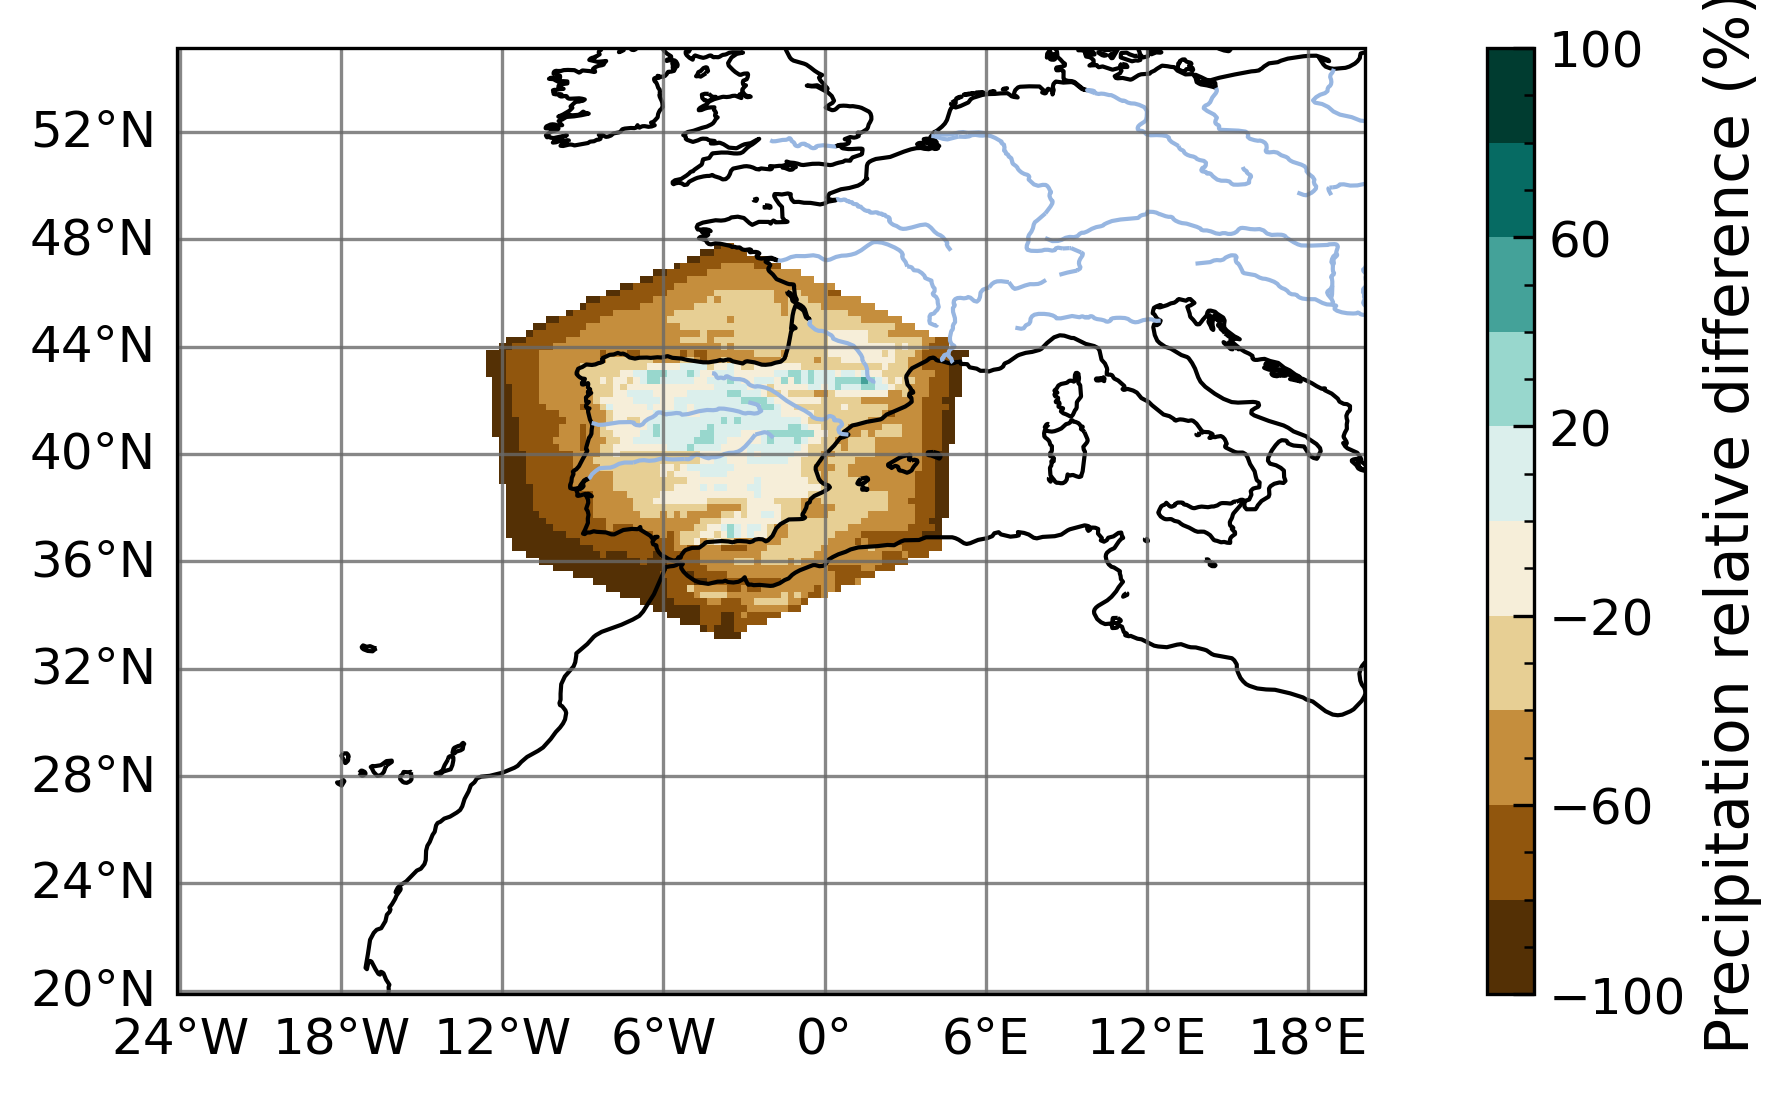
\includegraphics[width=\textwidth]{images/chap4/domain_size/rel_diff_map_precip_era_LAM_1000km_NBP40.png}
        \end{subfigure} &
        \begin{subfigure}[b]{0.33\textwidth}
            \caption{}
            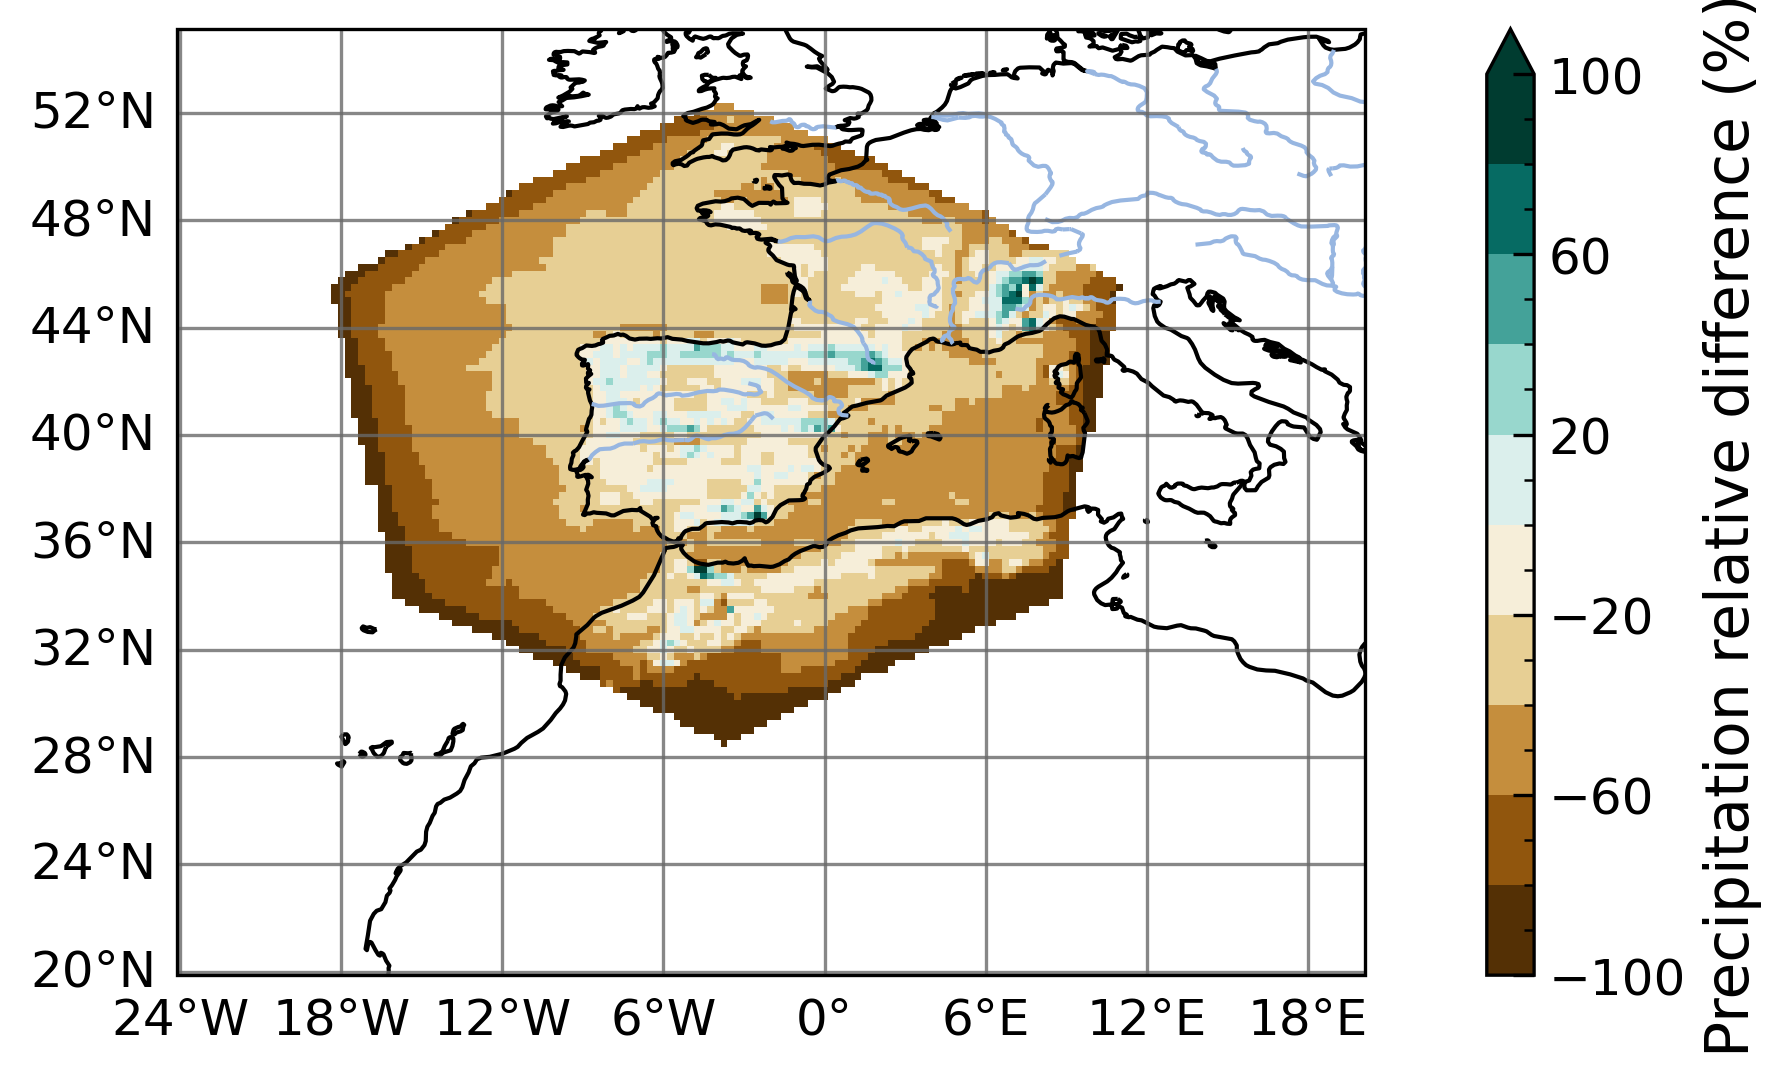
\includegraphics[width=\textwidth]{images/chap4/domain_size/rel_diff_map_precip_era_LAM_1500km_NBP60.png}
        \end{subfigure} &
        \begin{subfigure}[b]{0.33\textwidth}
            \caption{}
            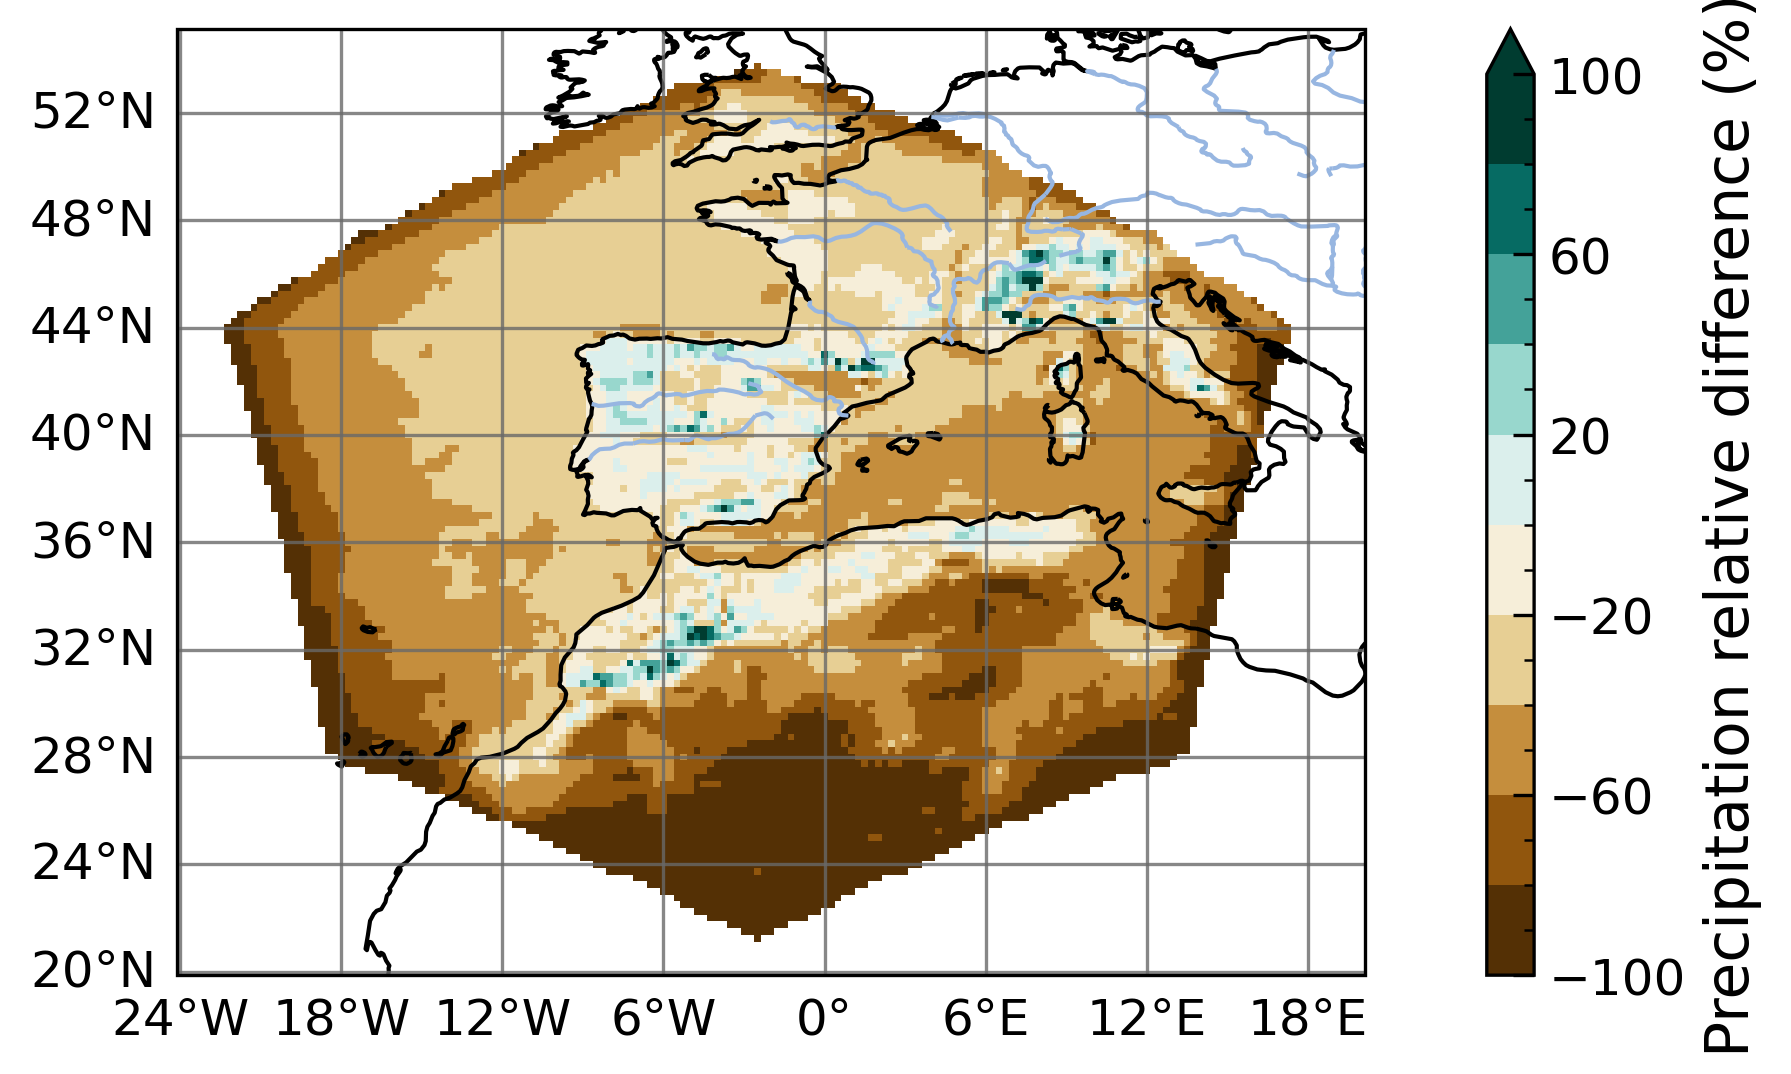
\includegraphics[width=\textwidth]{images/chap4/domain_size/rel_diff_map_precip_era_LAM_2000km_NBP80.png}
        \end{subfigure} \\
        
        %evap
        \begin{subfigure}[b]{0.33\textwidth}
            \caption{}
            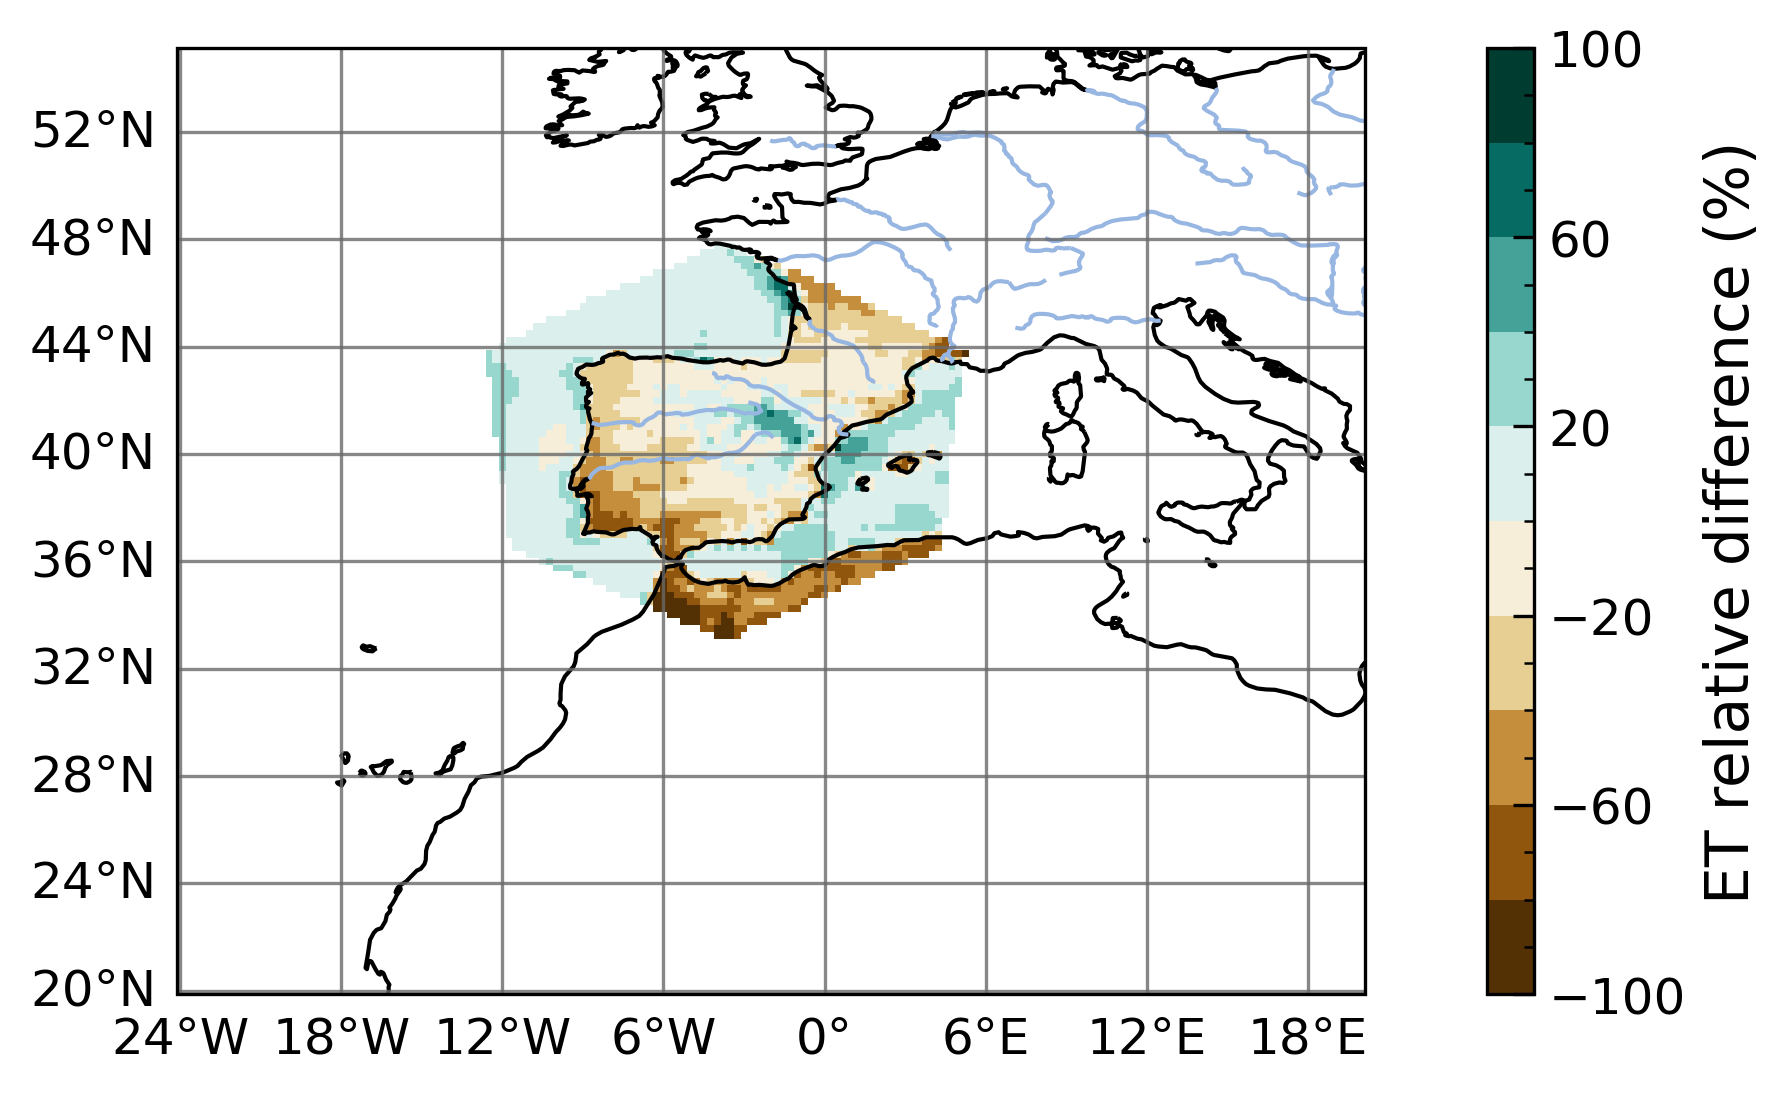
\includegraphics[width=\textwidth]{images/chap4/domain_size/rel_diff_map_evap_era_LAM_1000km_NBP40.png}
        \end{subfigure} &
        \begin{subfigure}[b]{0.33\textwidth}
            \caption{}
            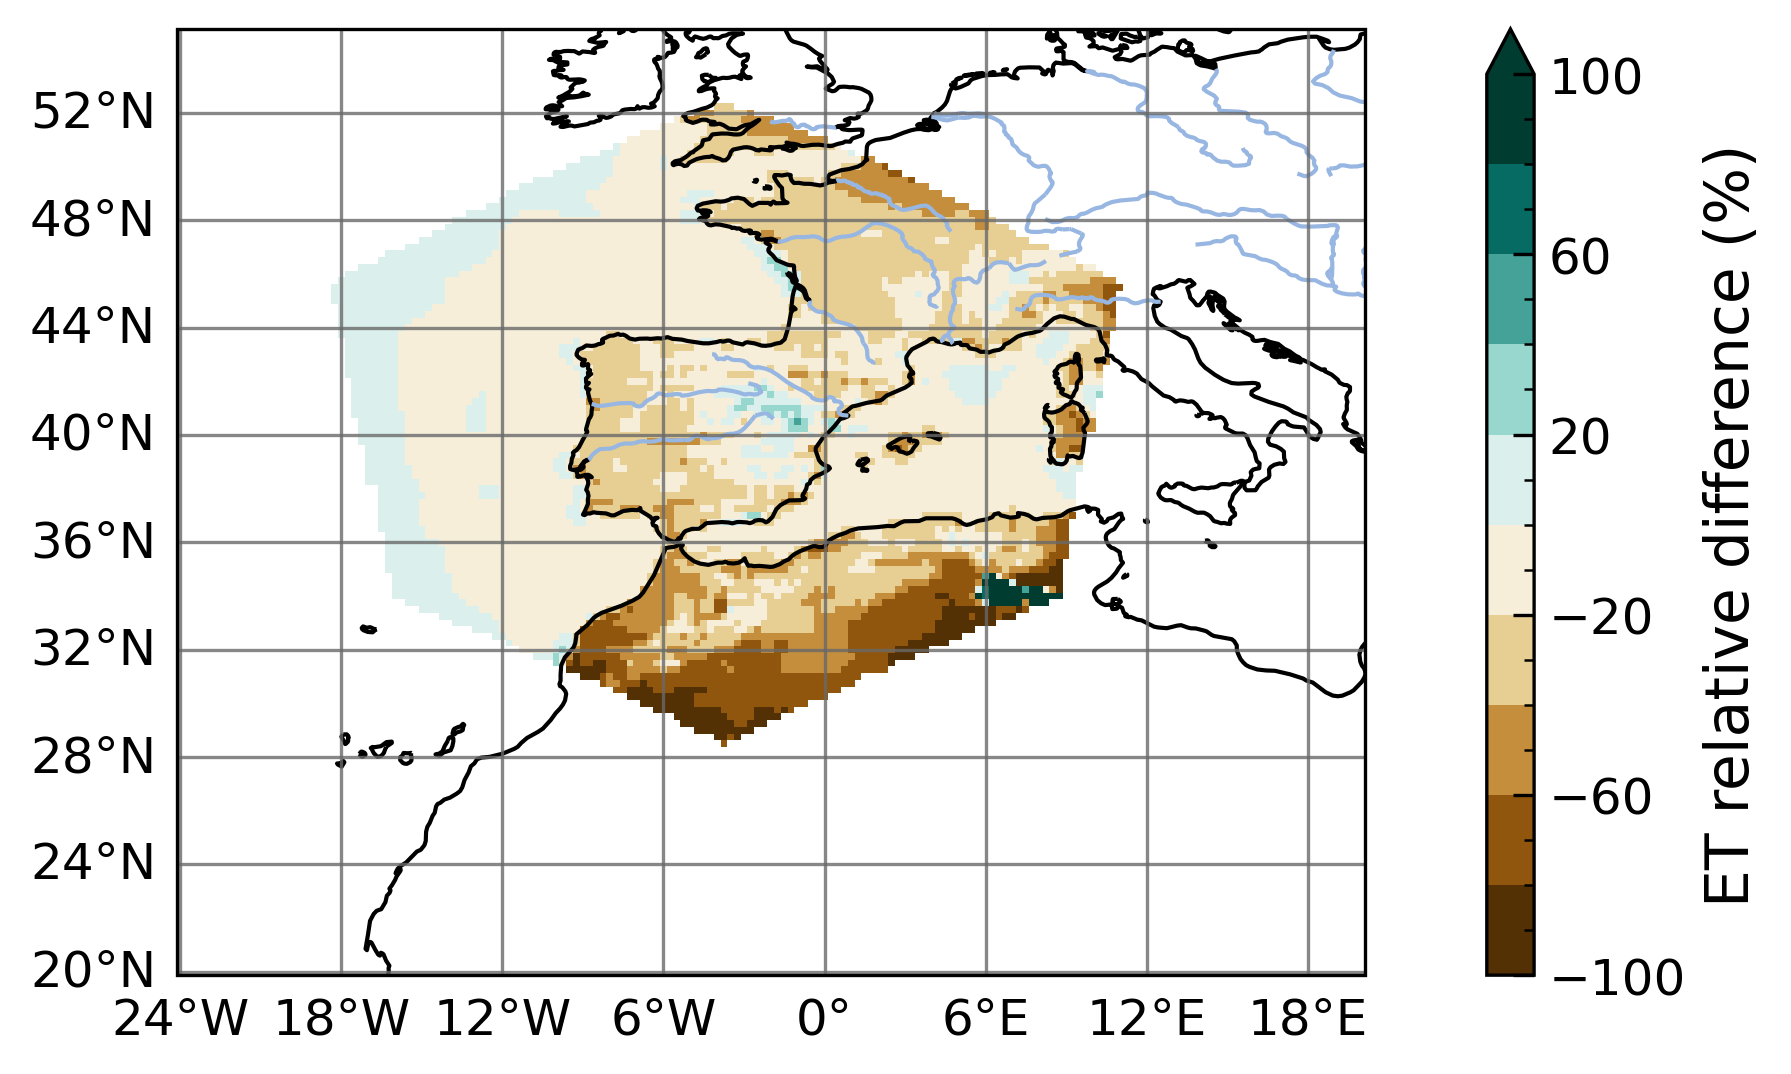
\includegraphics[width=\textwidth]{images/chap4/domain_size/rel_diff_map_evap_era_LAM_1500km_NBP60.png}
        \end{subfigure} &
        \begin{subfigure}[b]{0.33\textwidth}
            \caption{}
            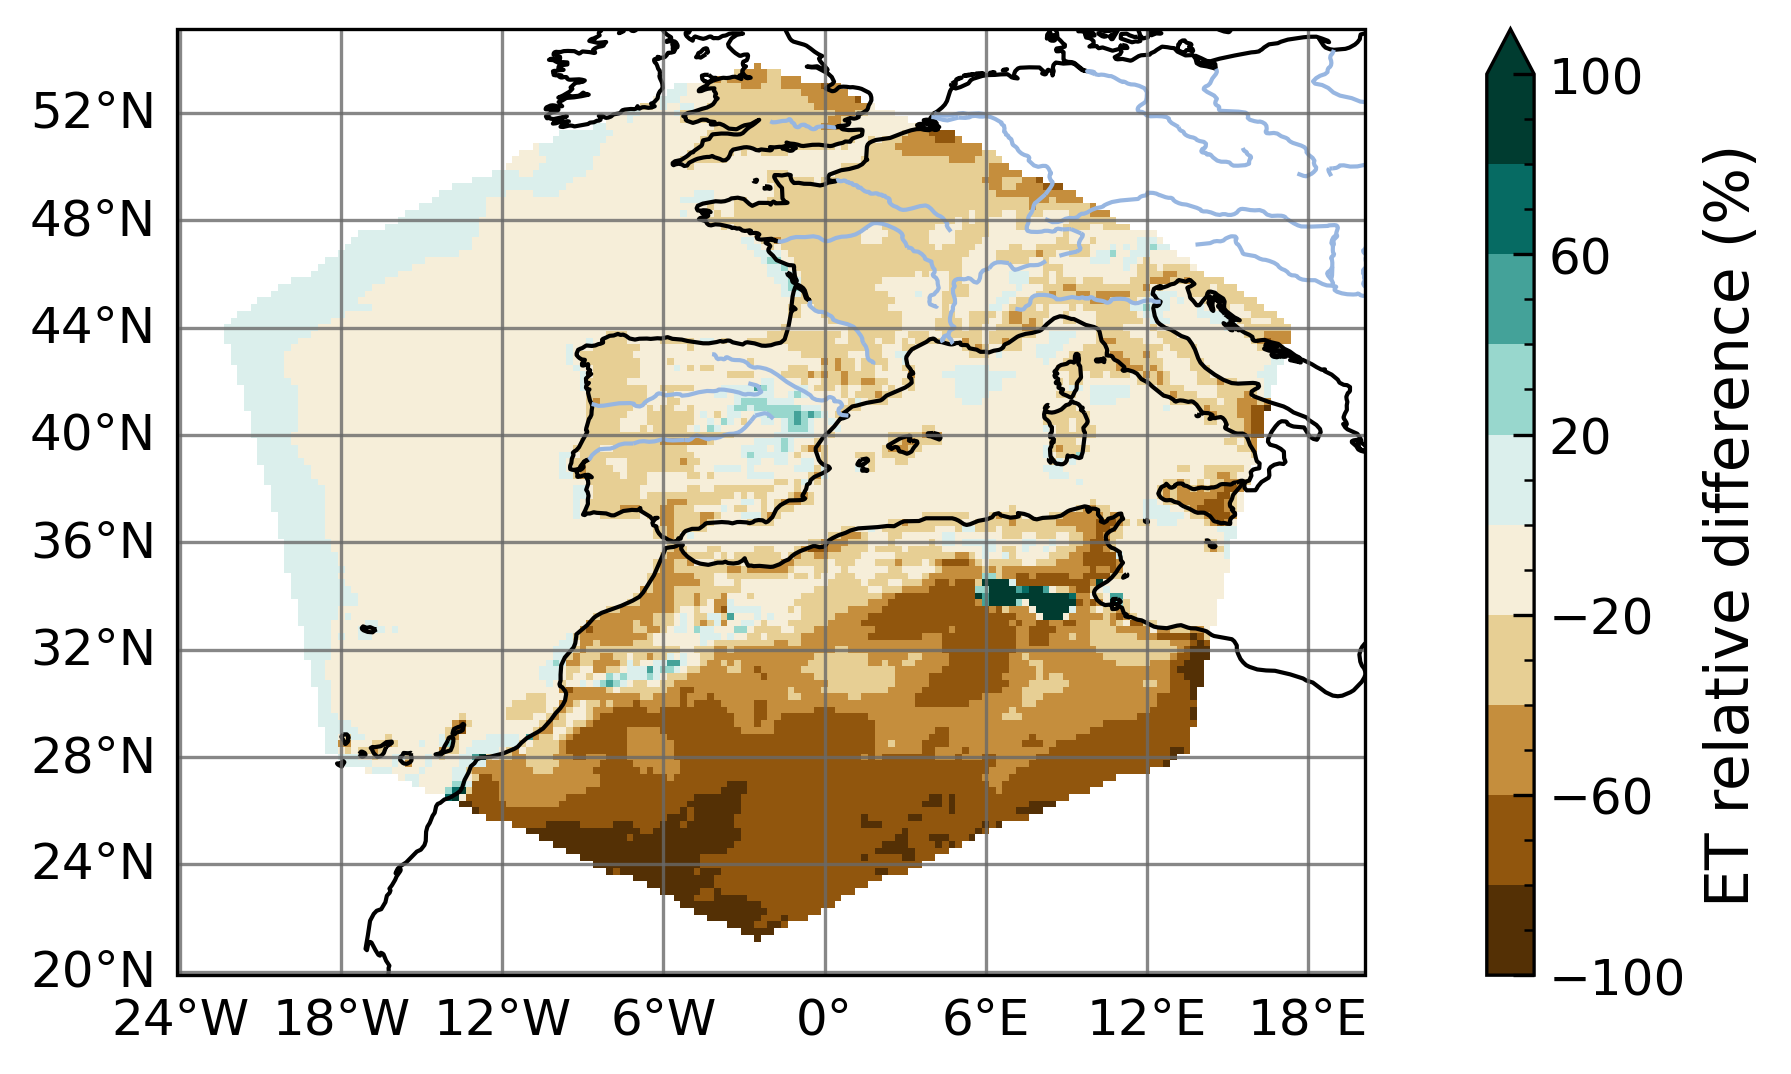
\includegraphics[width=\textwidth]{images/chap4/domain_size/rel_diff_map_evap_era_LAM_2000km_NBP80.png}
        \end{subfigure}
    \end{tabular}
    \caption{}
    \label{fig:domain_size_ERA_reldiff_maps}
\end{figure}
 
%f
\begin{figure}[htbp]
    \centering
    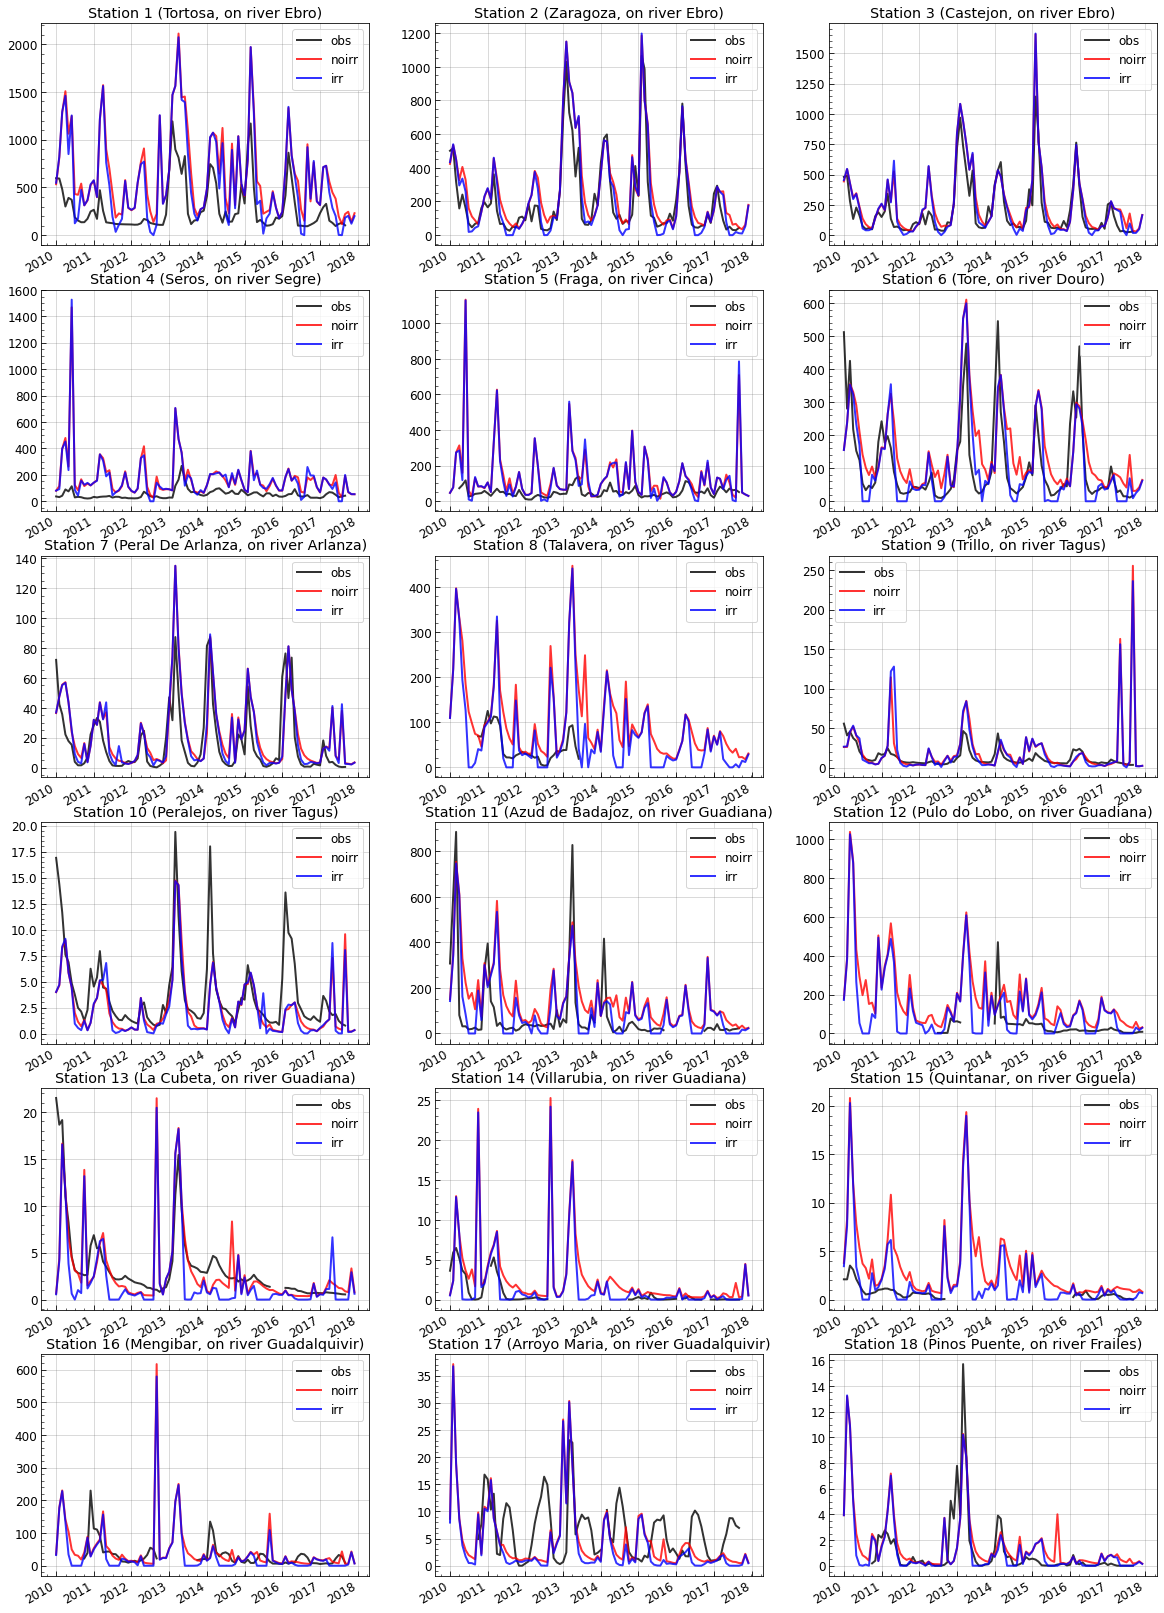
\includegraphics[width=\textwidth]{images/chap4/article/18_stations_TS.png}
    \caption{Time series of river discharge for the \irr and \noirr simulations and GRDC observations.}
    \label{fig:TS_discharge_18stations}
\end{figure}

%f
\begin{figure}[htbp]
    \centering
    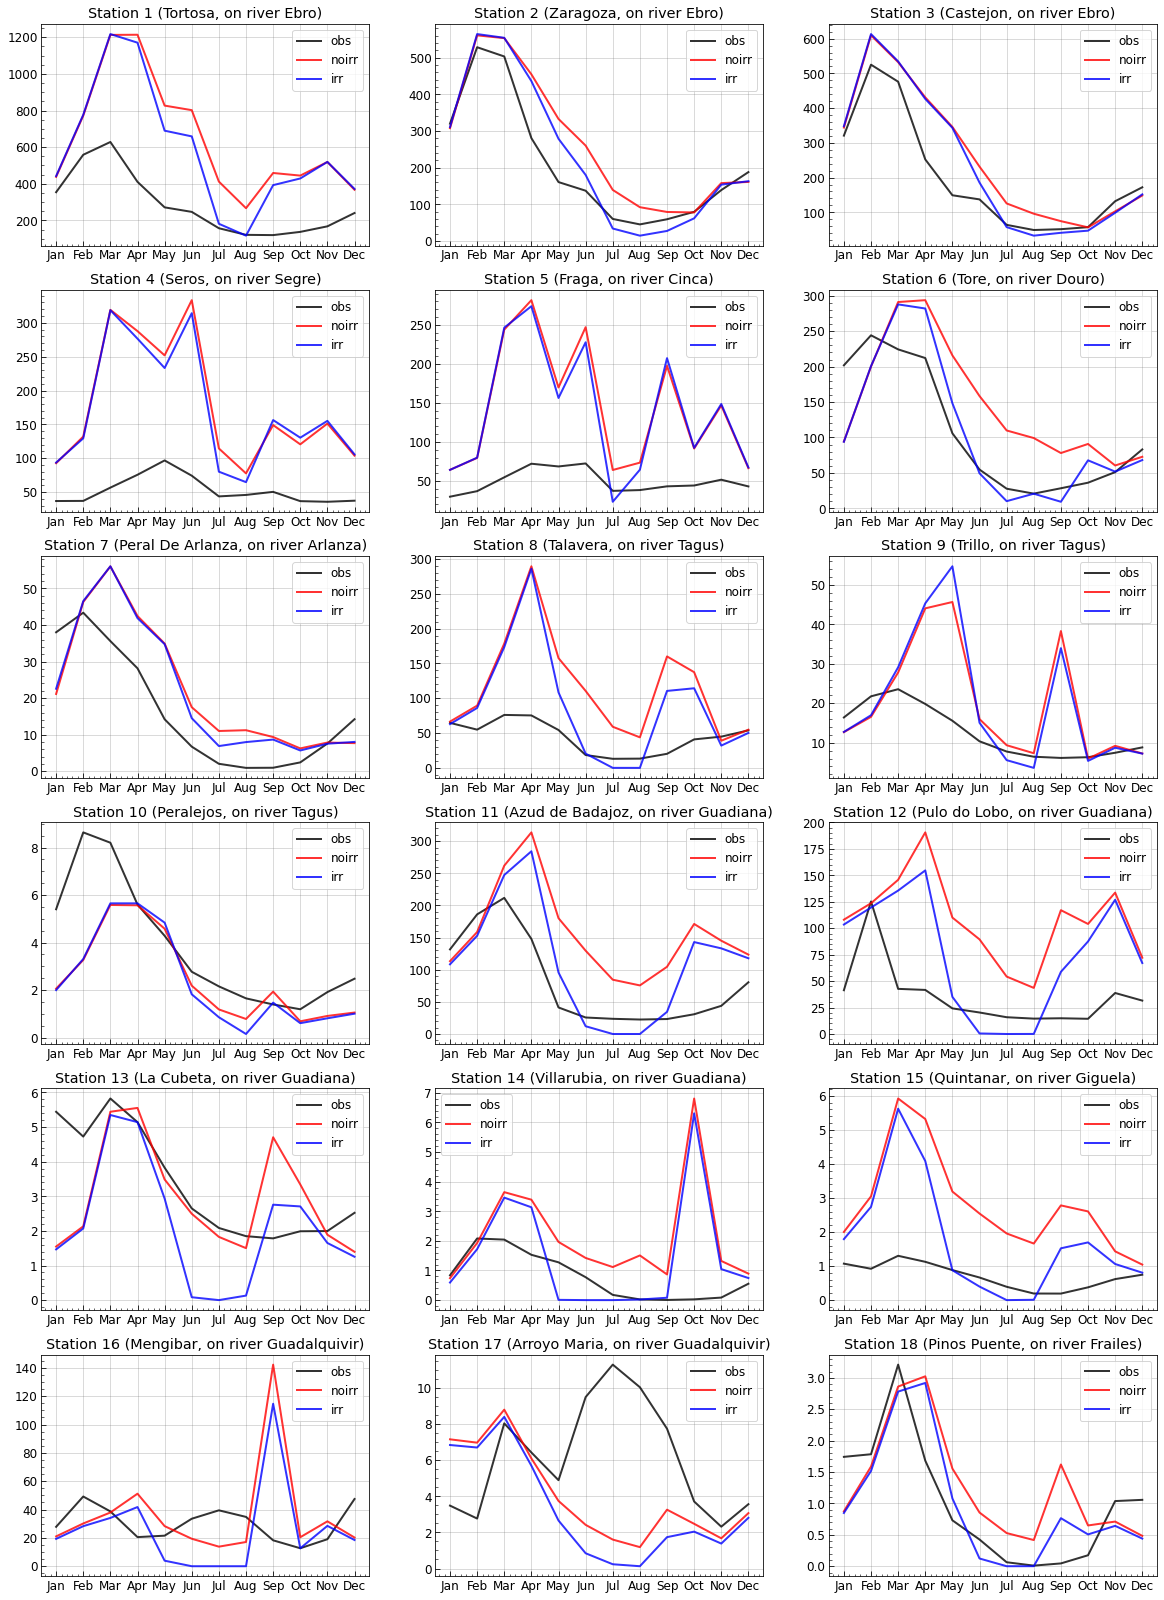
\includegraphics[width=\textwidth]{images/chap4/article/18_stations_SC.png}
    \caption{Mean seasonal cycle of river discharge for the \irr and \noirr simulations and GRDC observations. A mask is applied to the simulations to filter out months without corresponding observation data.}
    \label{fig:SC_discharge_18stations}
\end{figure}


%figure : from chap 4 future vs present. Seasonnal cycle of variables for 3 sims
\begin{figure}[htbp]
    \centering
    \begin{tabular}{cc}
        %precip
        \begin{subfigure}[b]{0.5\textwidth}
            \caption{}
            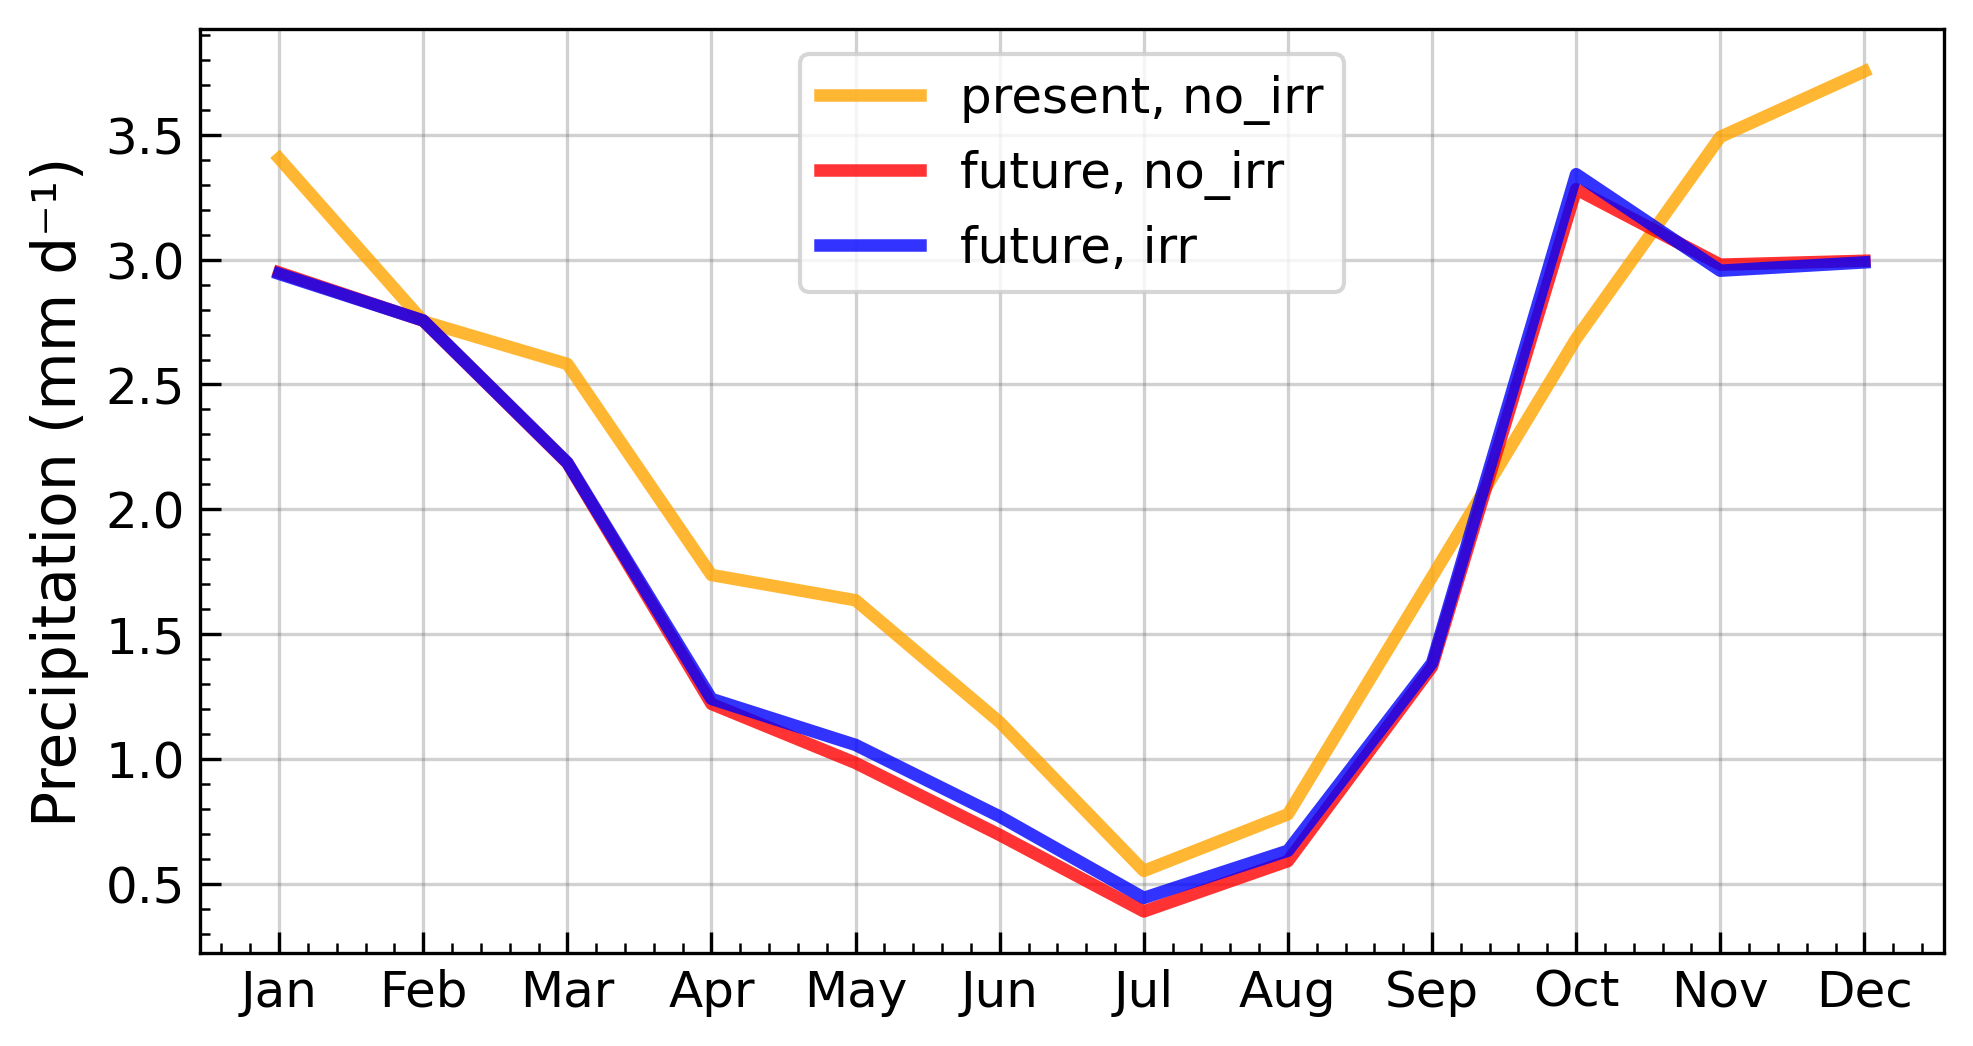
\includegraphics[width=\textwidth]{images/chap4/future/SC_precip_presfutirr.png}
        \end{subfigure} &
        %evap
        \begin{subfigure}[b]{0.5\textwidth}
            \caption{}
            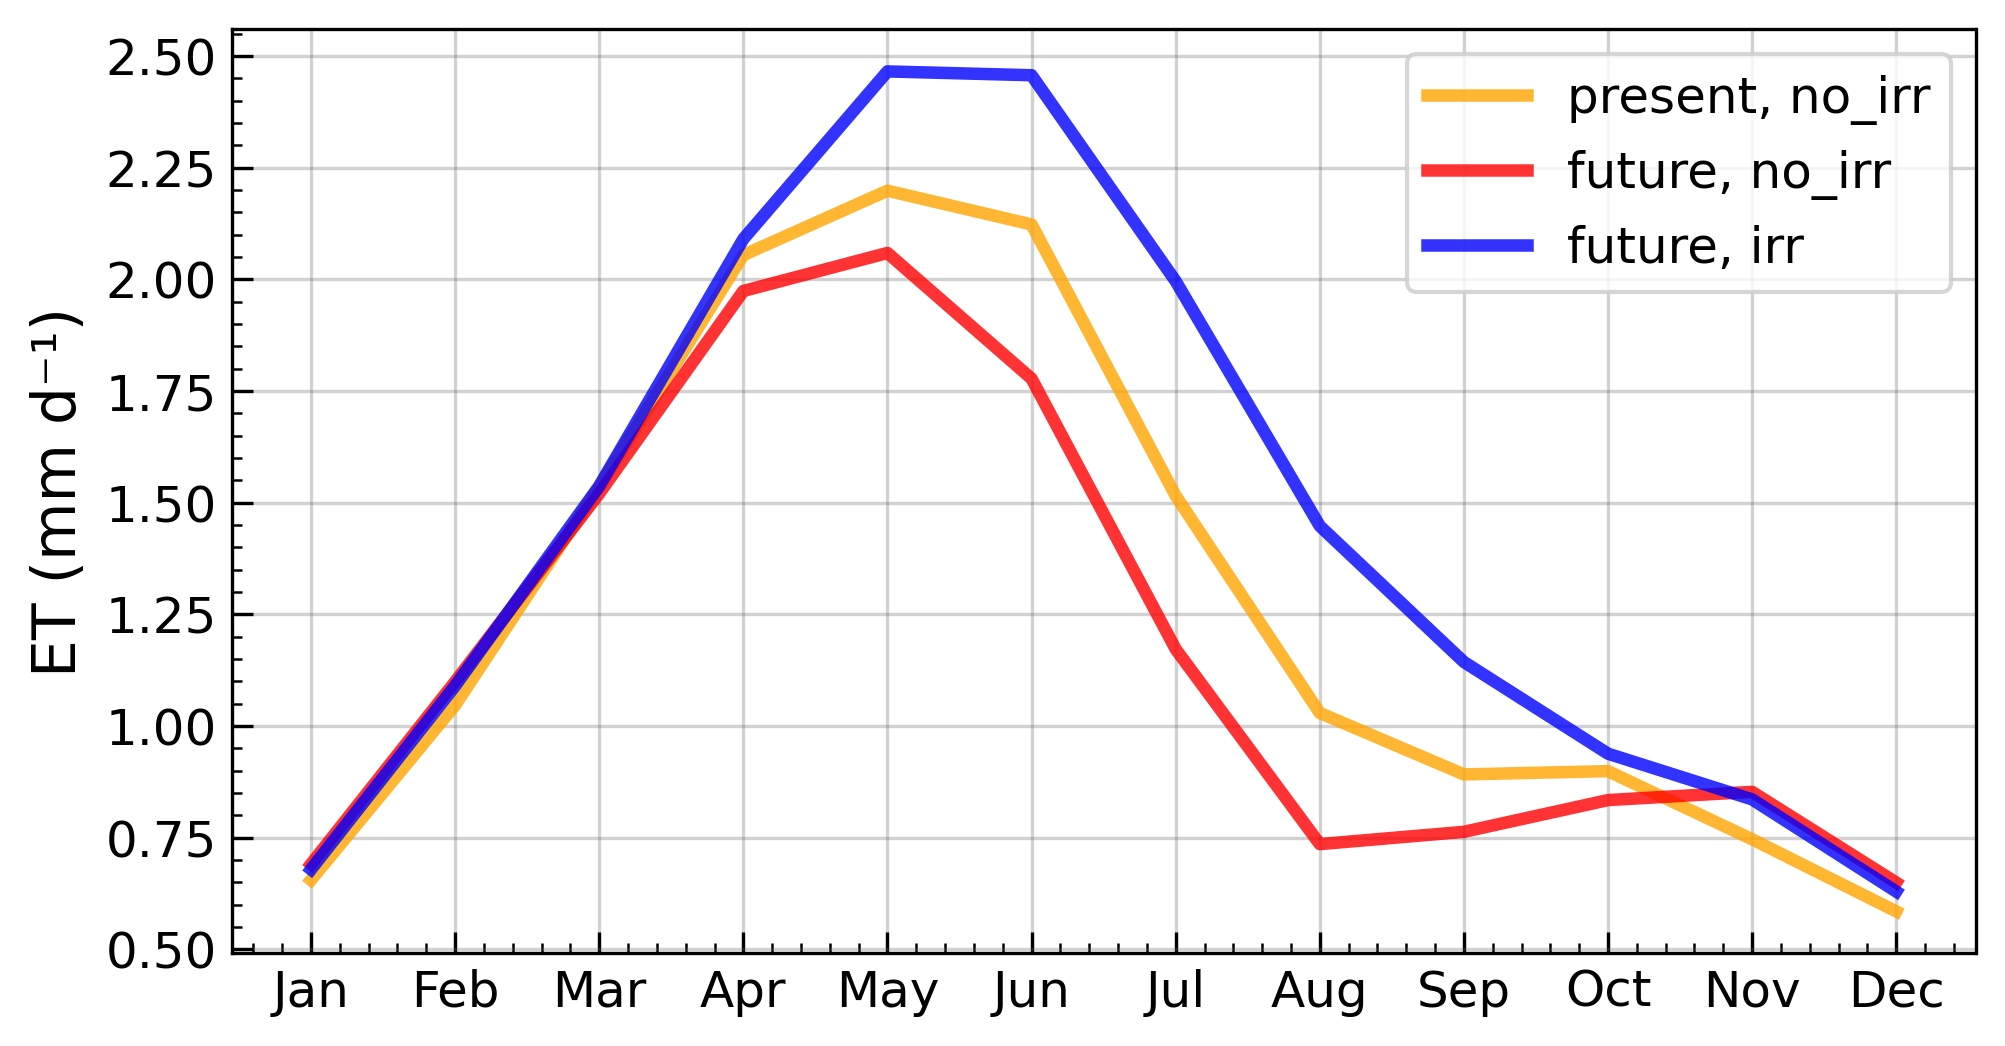
\includegraphics[width=\textwidth]{images/chap4/future/SC_evap_presfutirr.png}
        \end{subfigure} \\

        %t2m
        \begin{subfigure}[b]{0.5\textwidth}
            \caption{}
            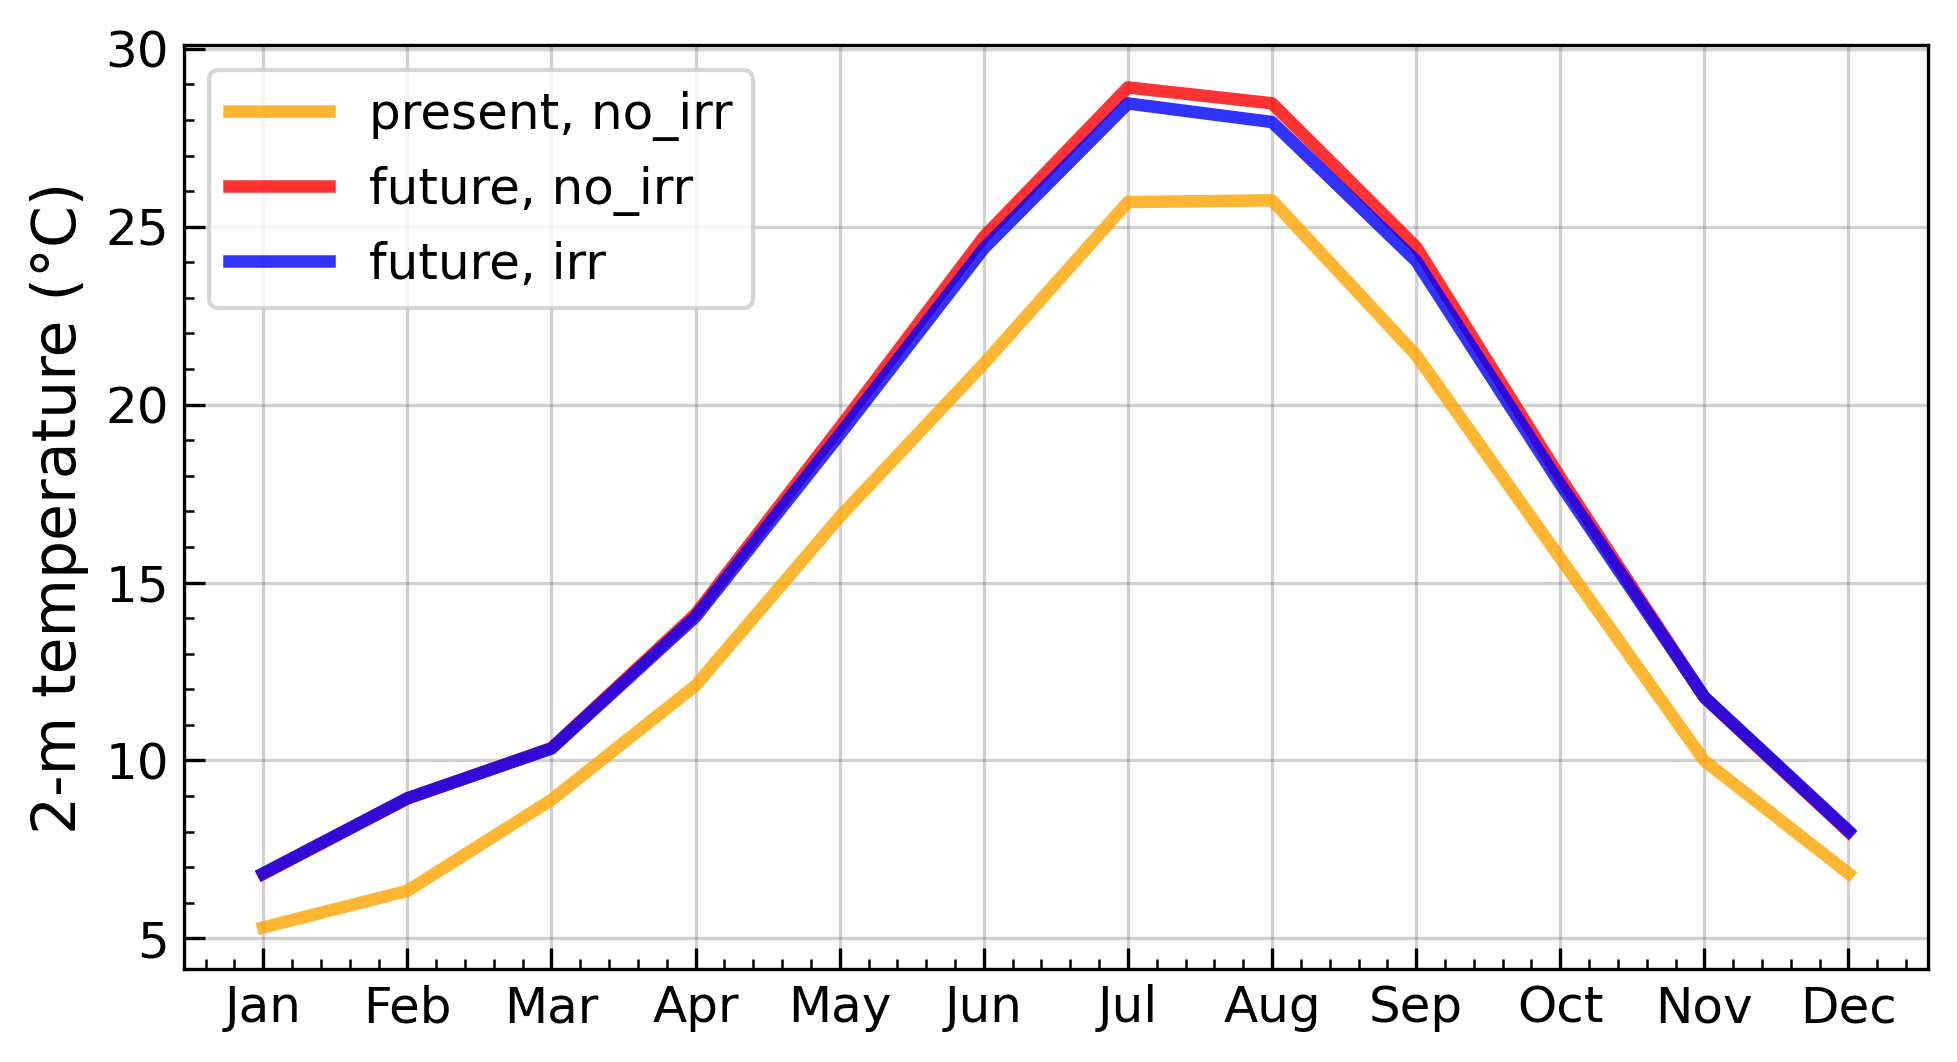
\includegraphics[width=\textwidth]{images/chap4/future/SC_t2m_presfutirr.png}
        \end{subfigure} &
        %fluxsens
        \begin{subfigure}[b]{0.5\textwidth}
            \caption{}
            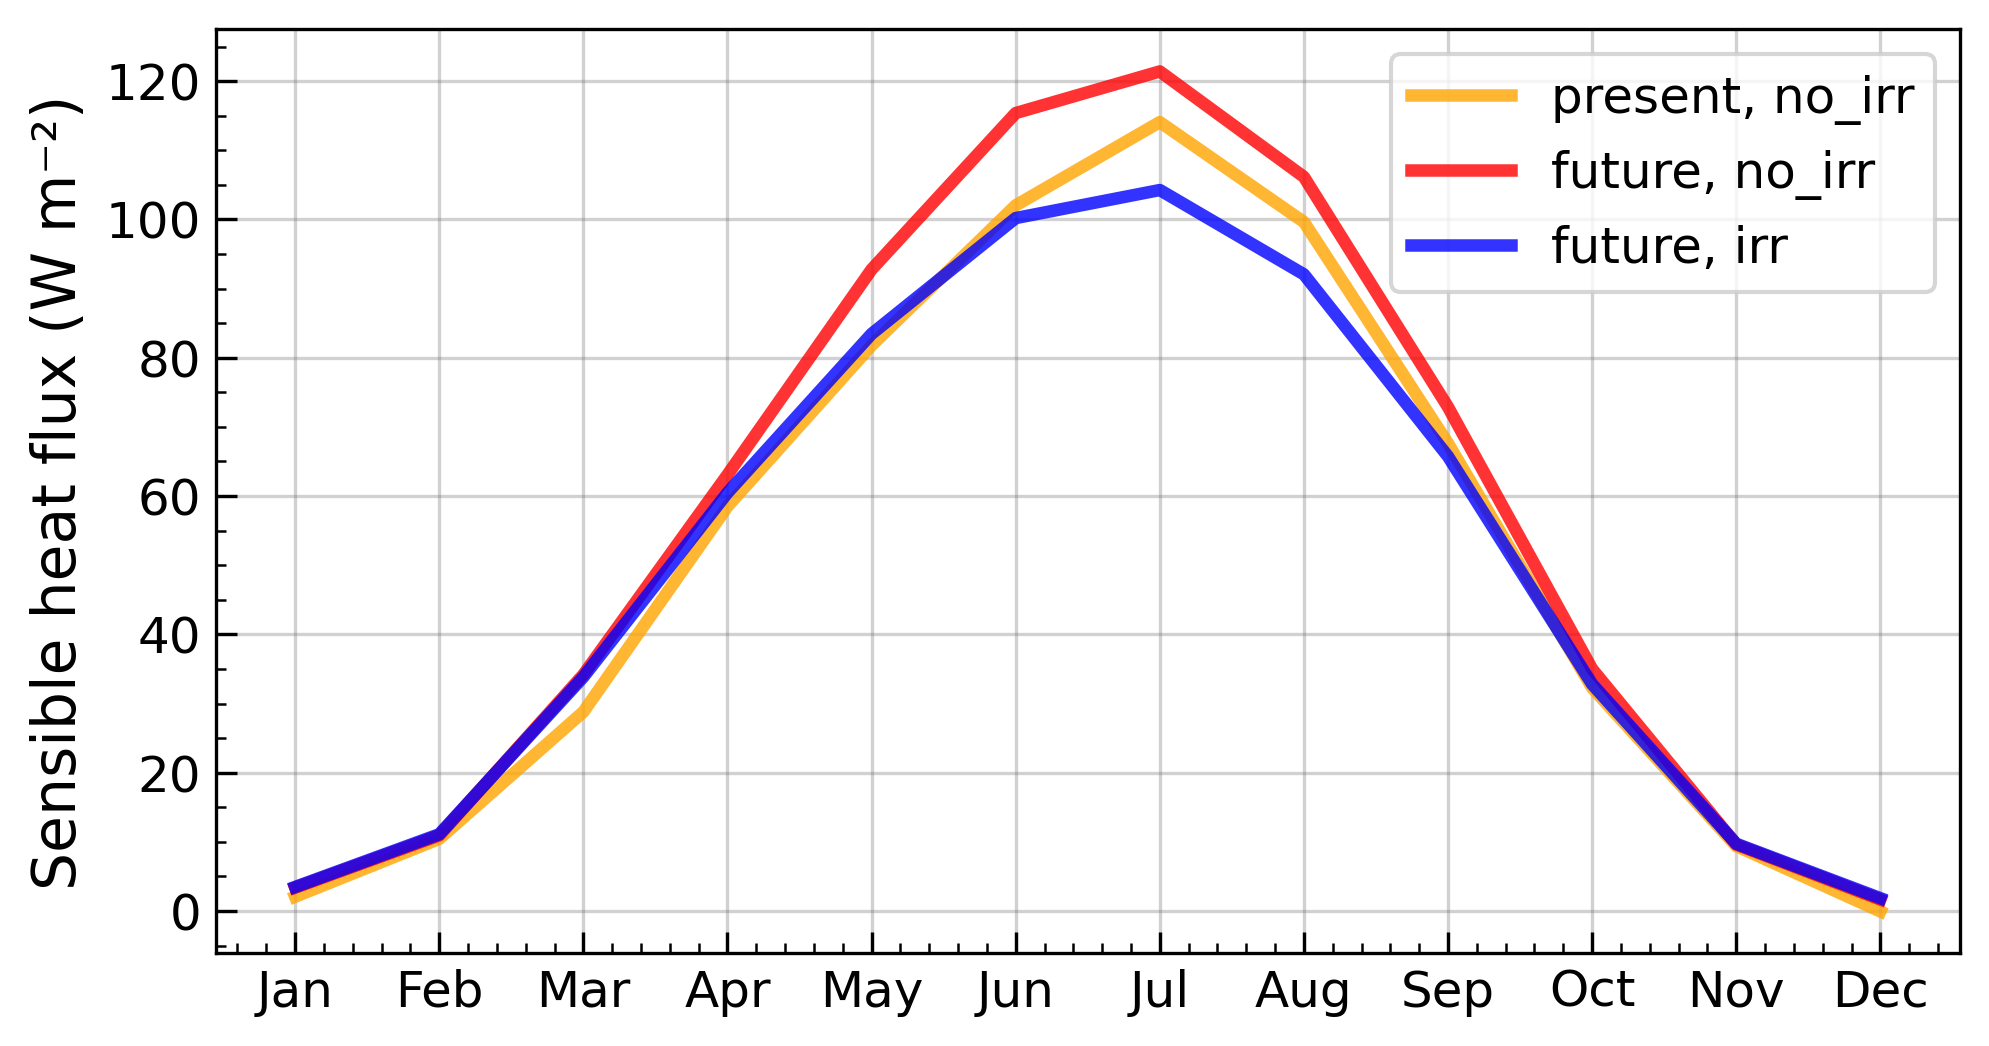
\includegraphics[width=\textwidth]{images/chap4/future/SC_fluxsens_presfutirr.png}
        \end{subfigure} \\

        %q2m
        \begin{subfigure}[b]{0.5\textwidth}
            \caption{}
            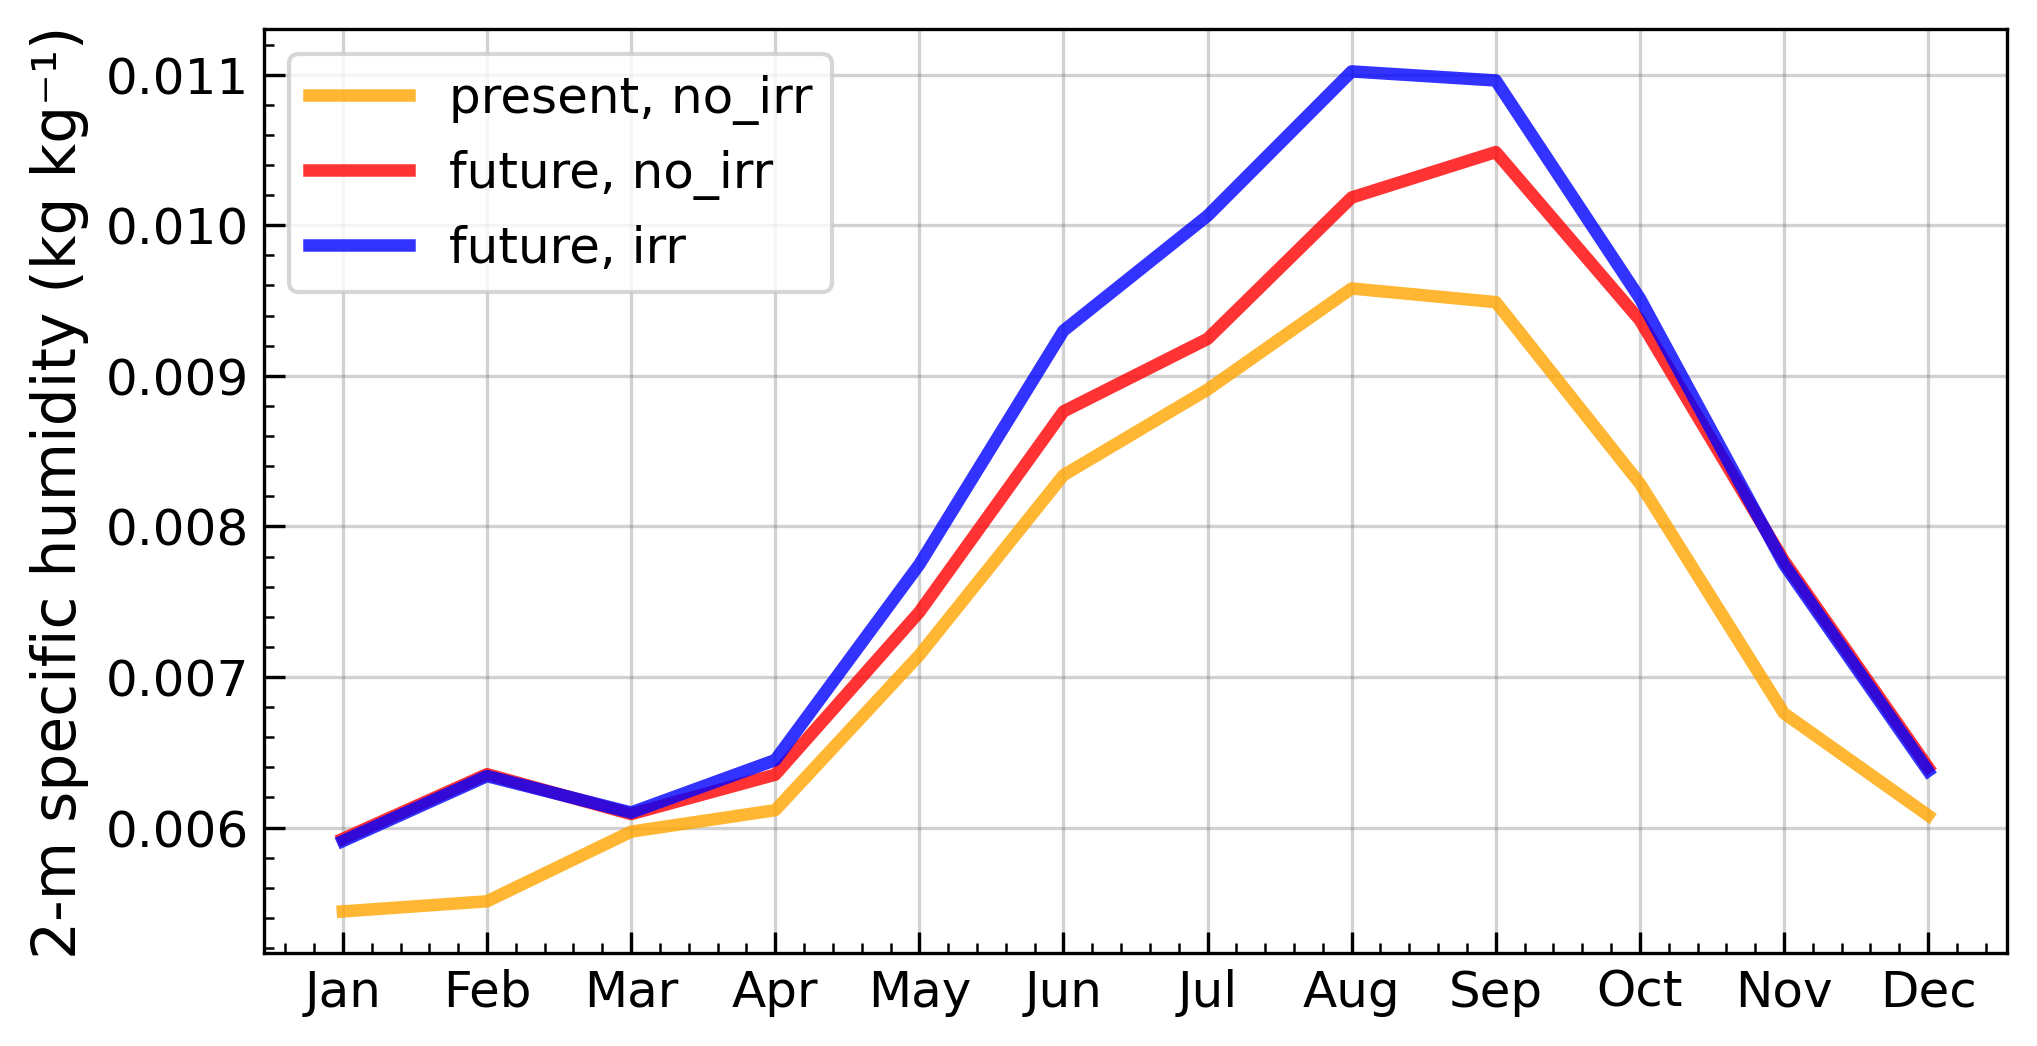
\includegraphics[width=\textwidth]{images/chap4/future/SC_q2m_presfutirr.png}
        \end{subfigure} &
        %rh2m
        \begin{subfigure}[b]{0.5\textwidth}
            \caption{}
            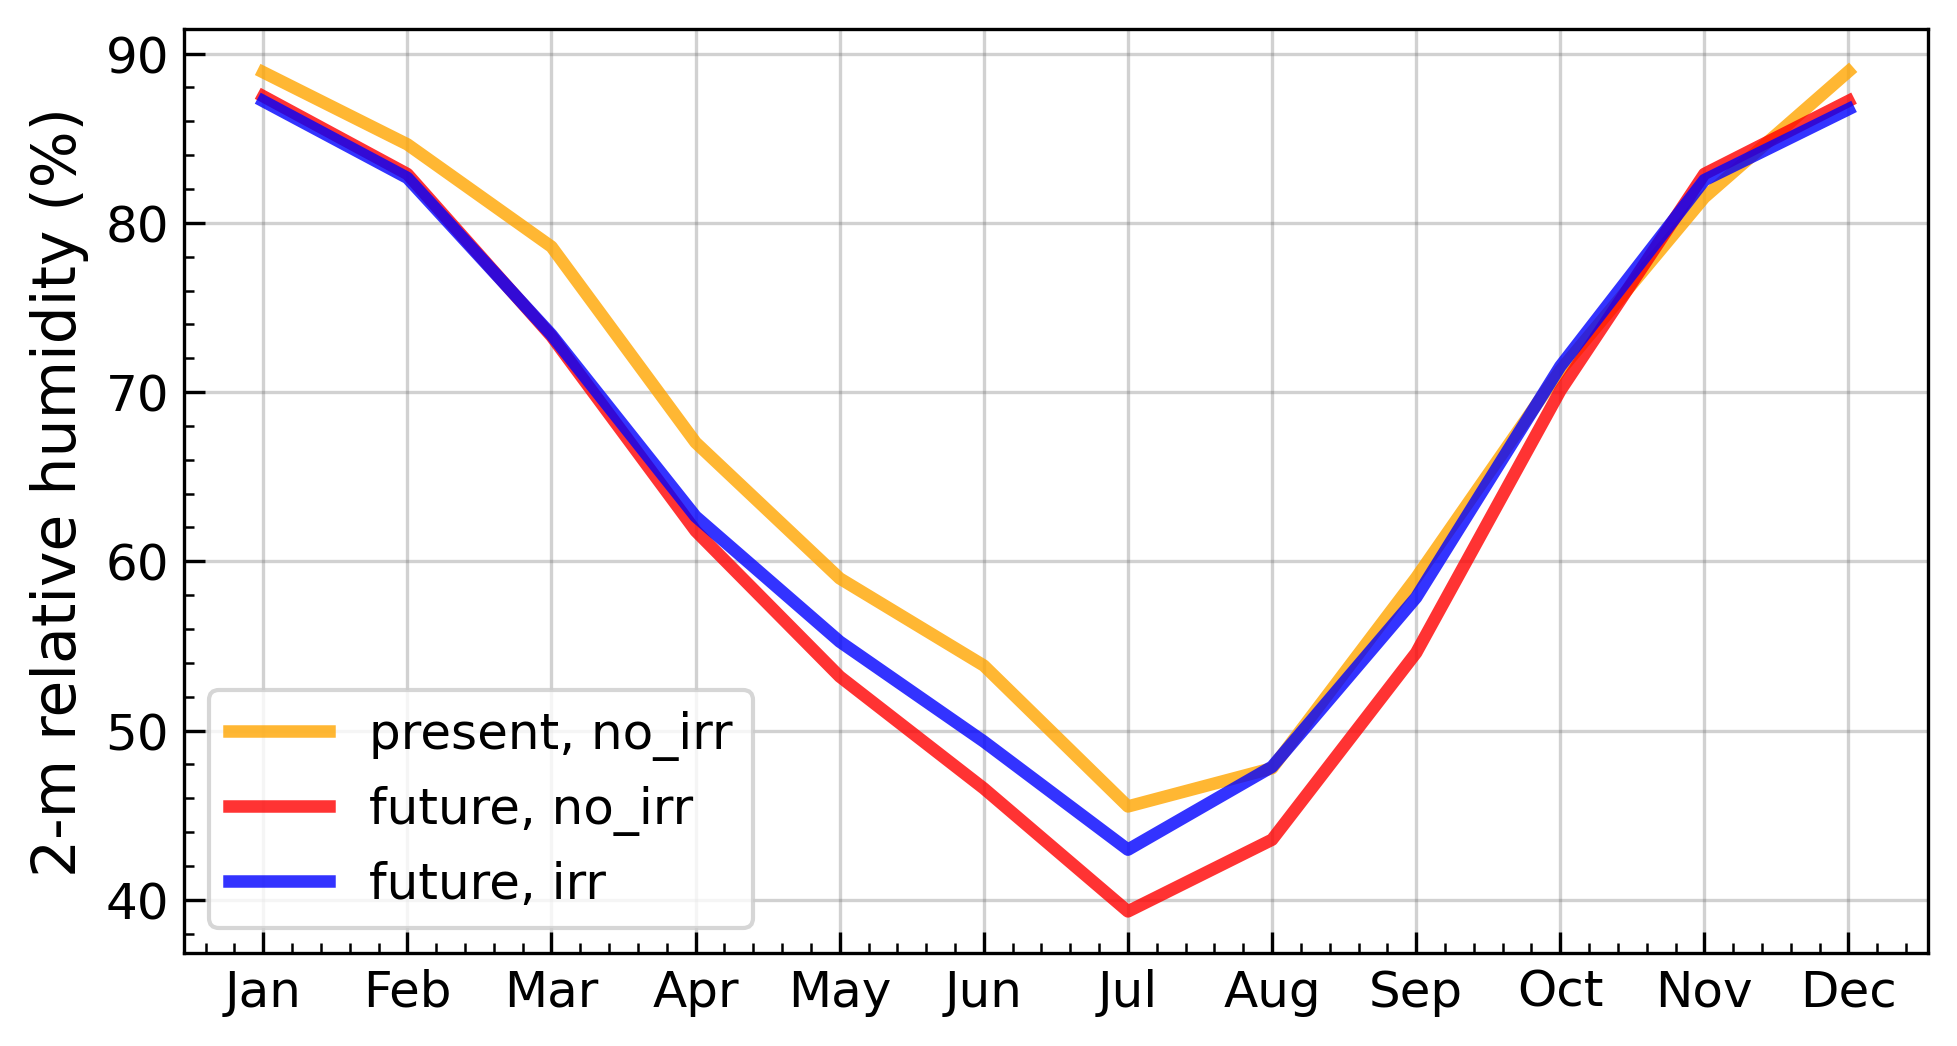
\includegraphics[width=\textwidth]{images/chap4/future/SC_rh2m_presfutirr.png}
        \end{subfigure} \\

        %pblh
        \begin{subfigure}[b]{0.5\textwidth}
            \caption{}
            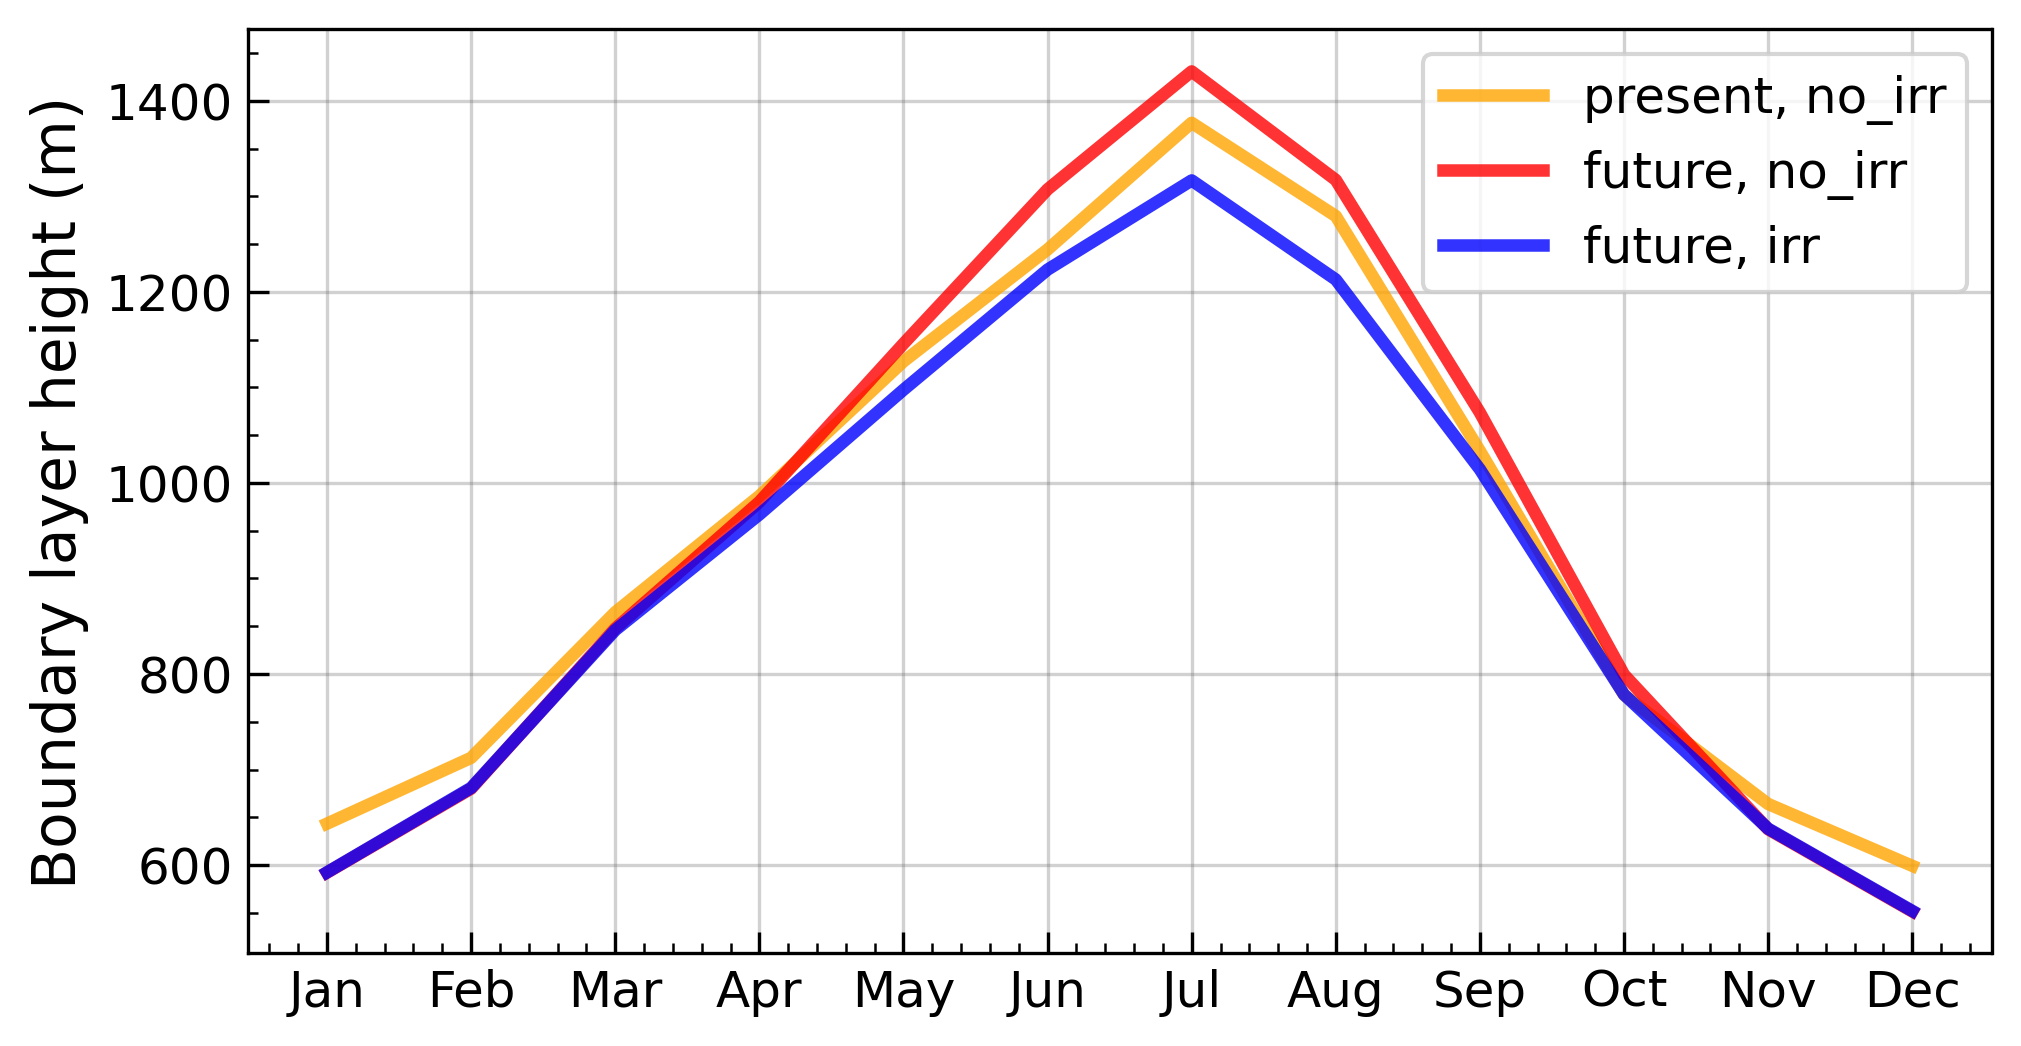
\includegraphics[width=\textwidth]{images/chap4/future/SC_s_pblh_presfutirr.png}
        \end{subfigure} &
        %lcl
        \begin{subfigure}[b]{0.5\textwidth}
            \caption{}
            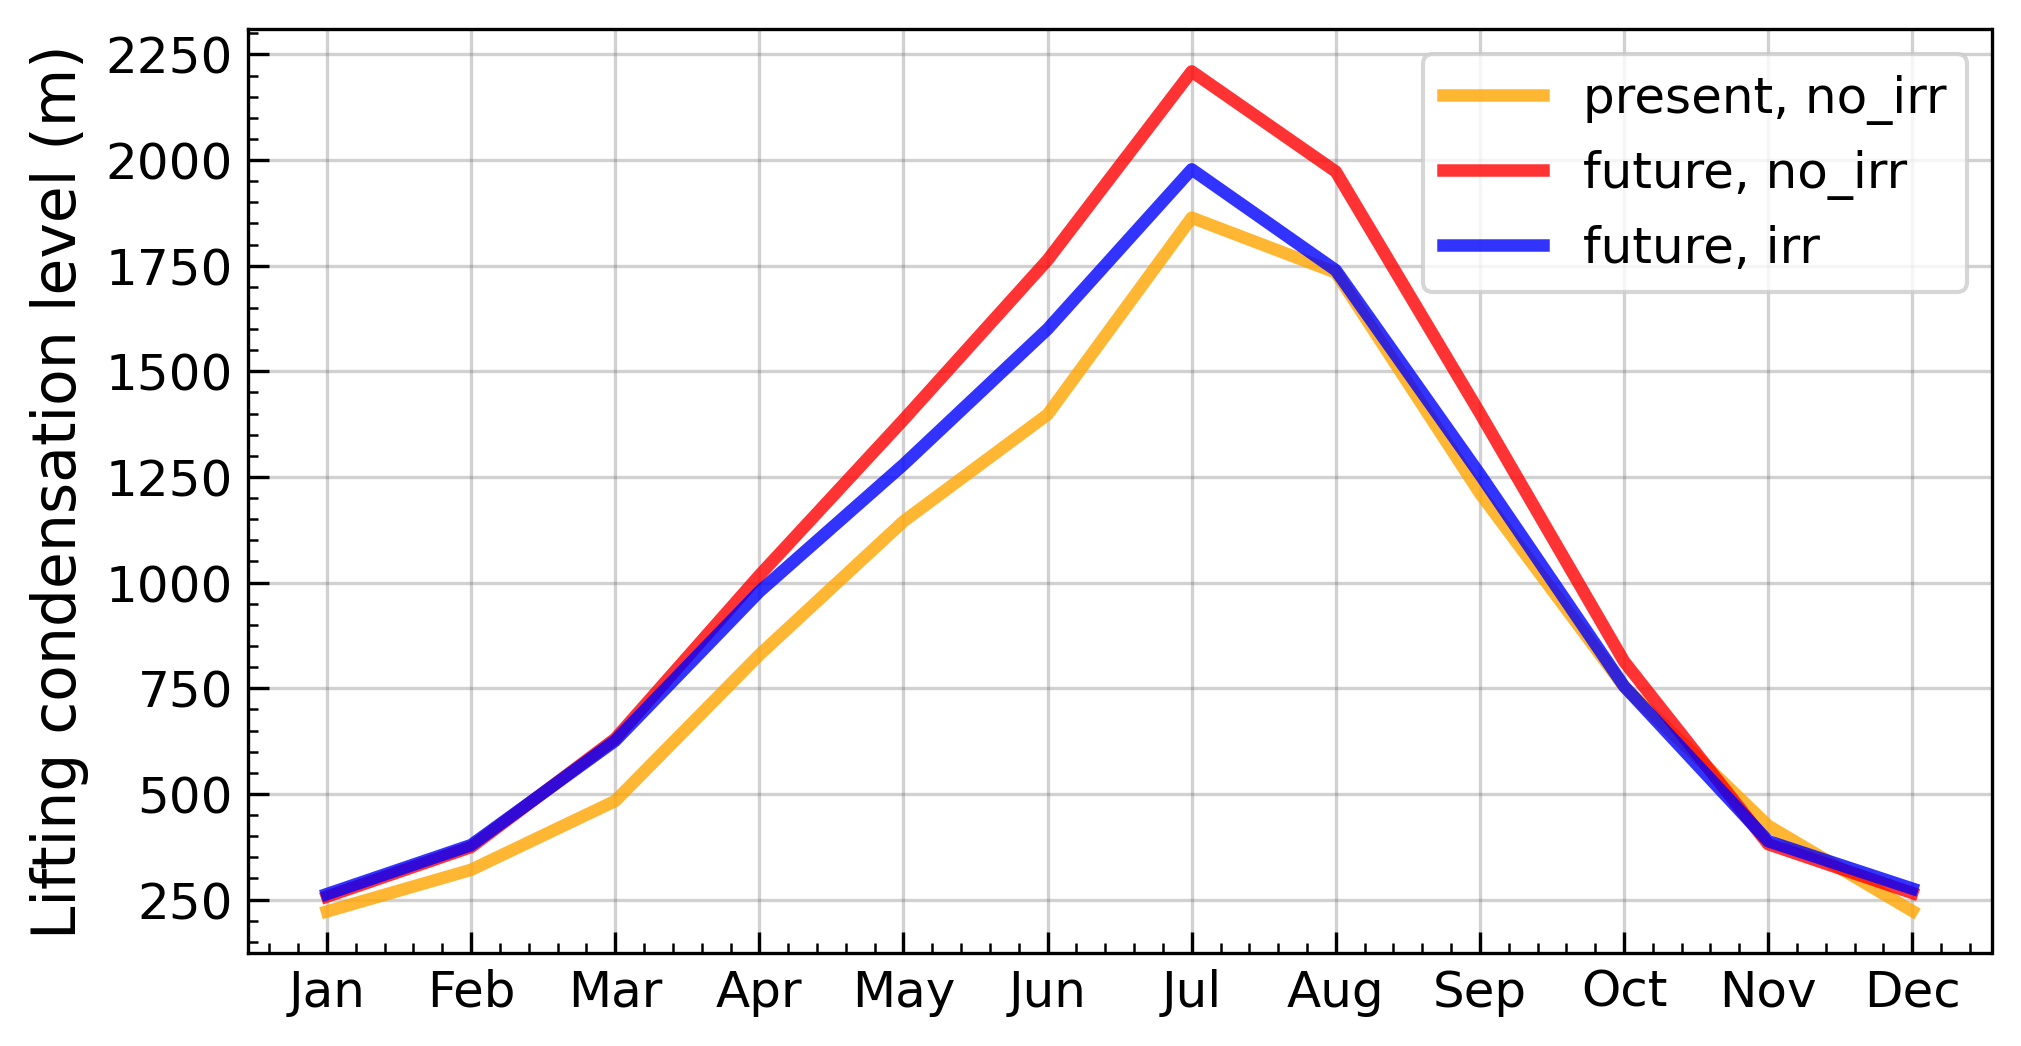
\includegraphics[width=\textwidth]{images/chap4/future/SC_s_lcl_presfutirr.png}
        \end{subfigure} \\
    \end{tabular}
    \caption{}
    \label{fig:diffmaps_future_irr}
\end{figure}

%figure : diff maps JJA (noirr, pres - future)
\begin{figure}[htbp]
    \centering
    \begin{tabular}{cc}
        %precip
        \begin{subfigure}[b]{0.5\textwidth}
            \caption{}
            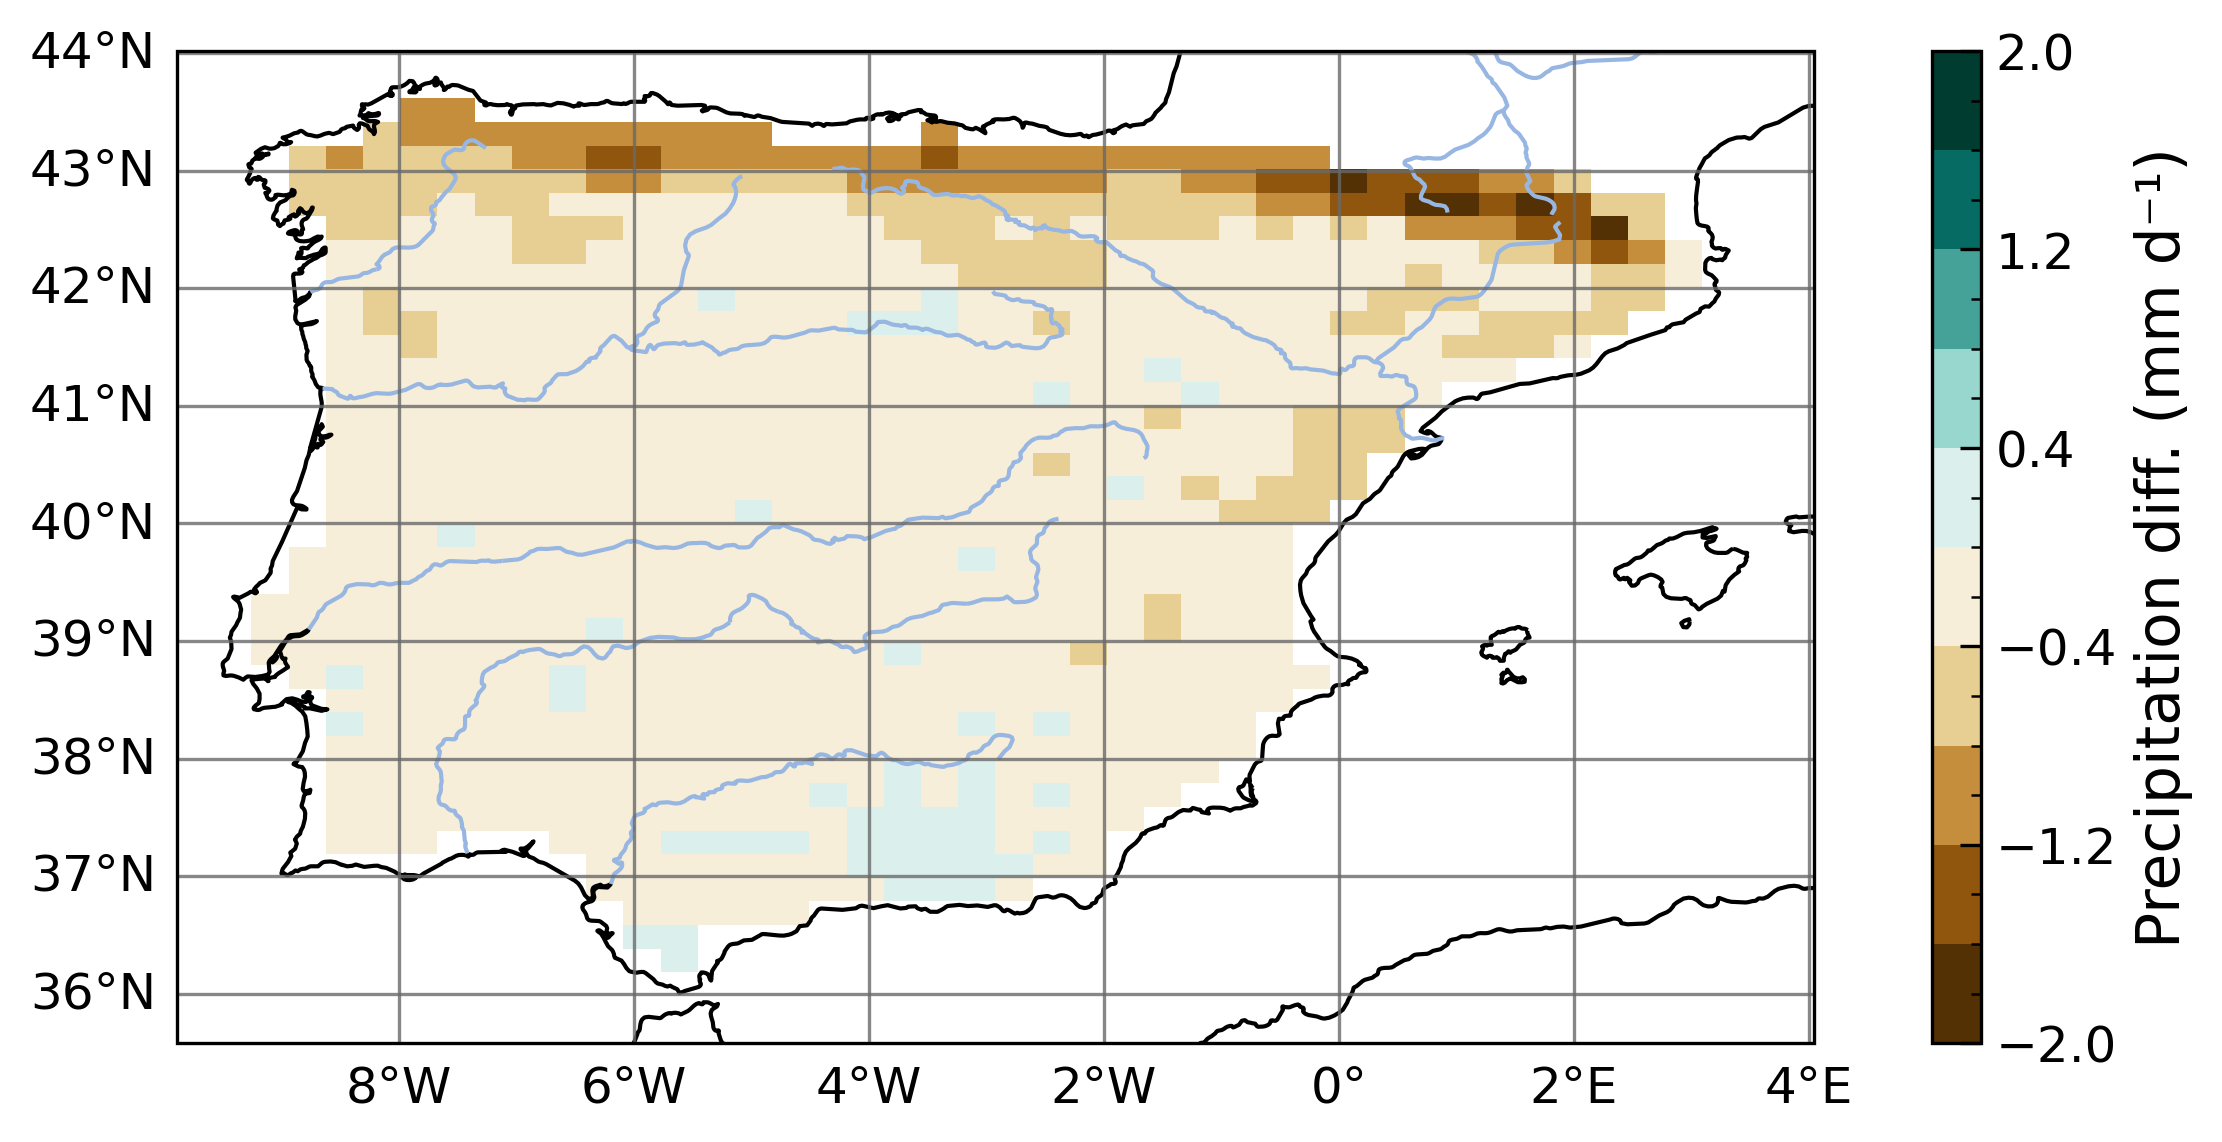
\includegraphics[width=\textwidth]{images/chap4/future/diffmap_JJA_precip_presfut.png}
        \end{subfigure} &
        %evap
        \begin{subfigure}[b]{0.5\textwidth}
            \caption{}
            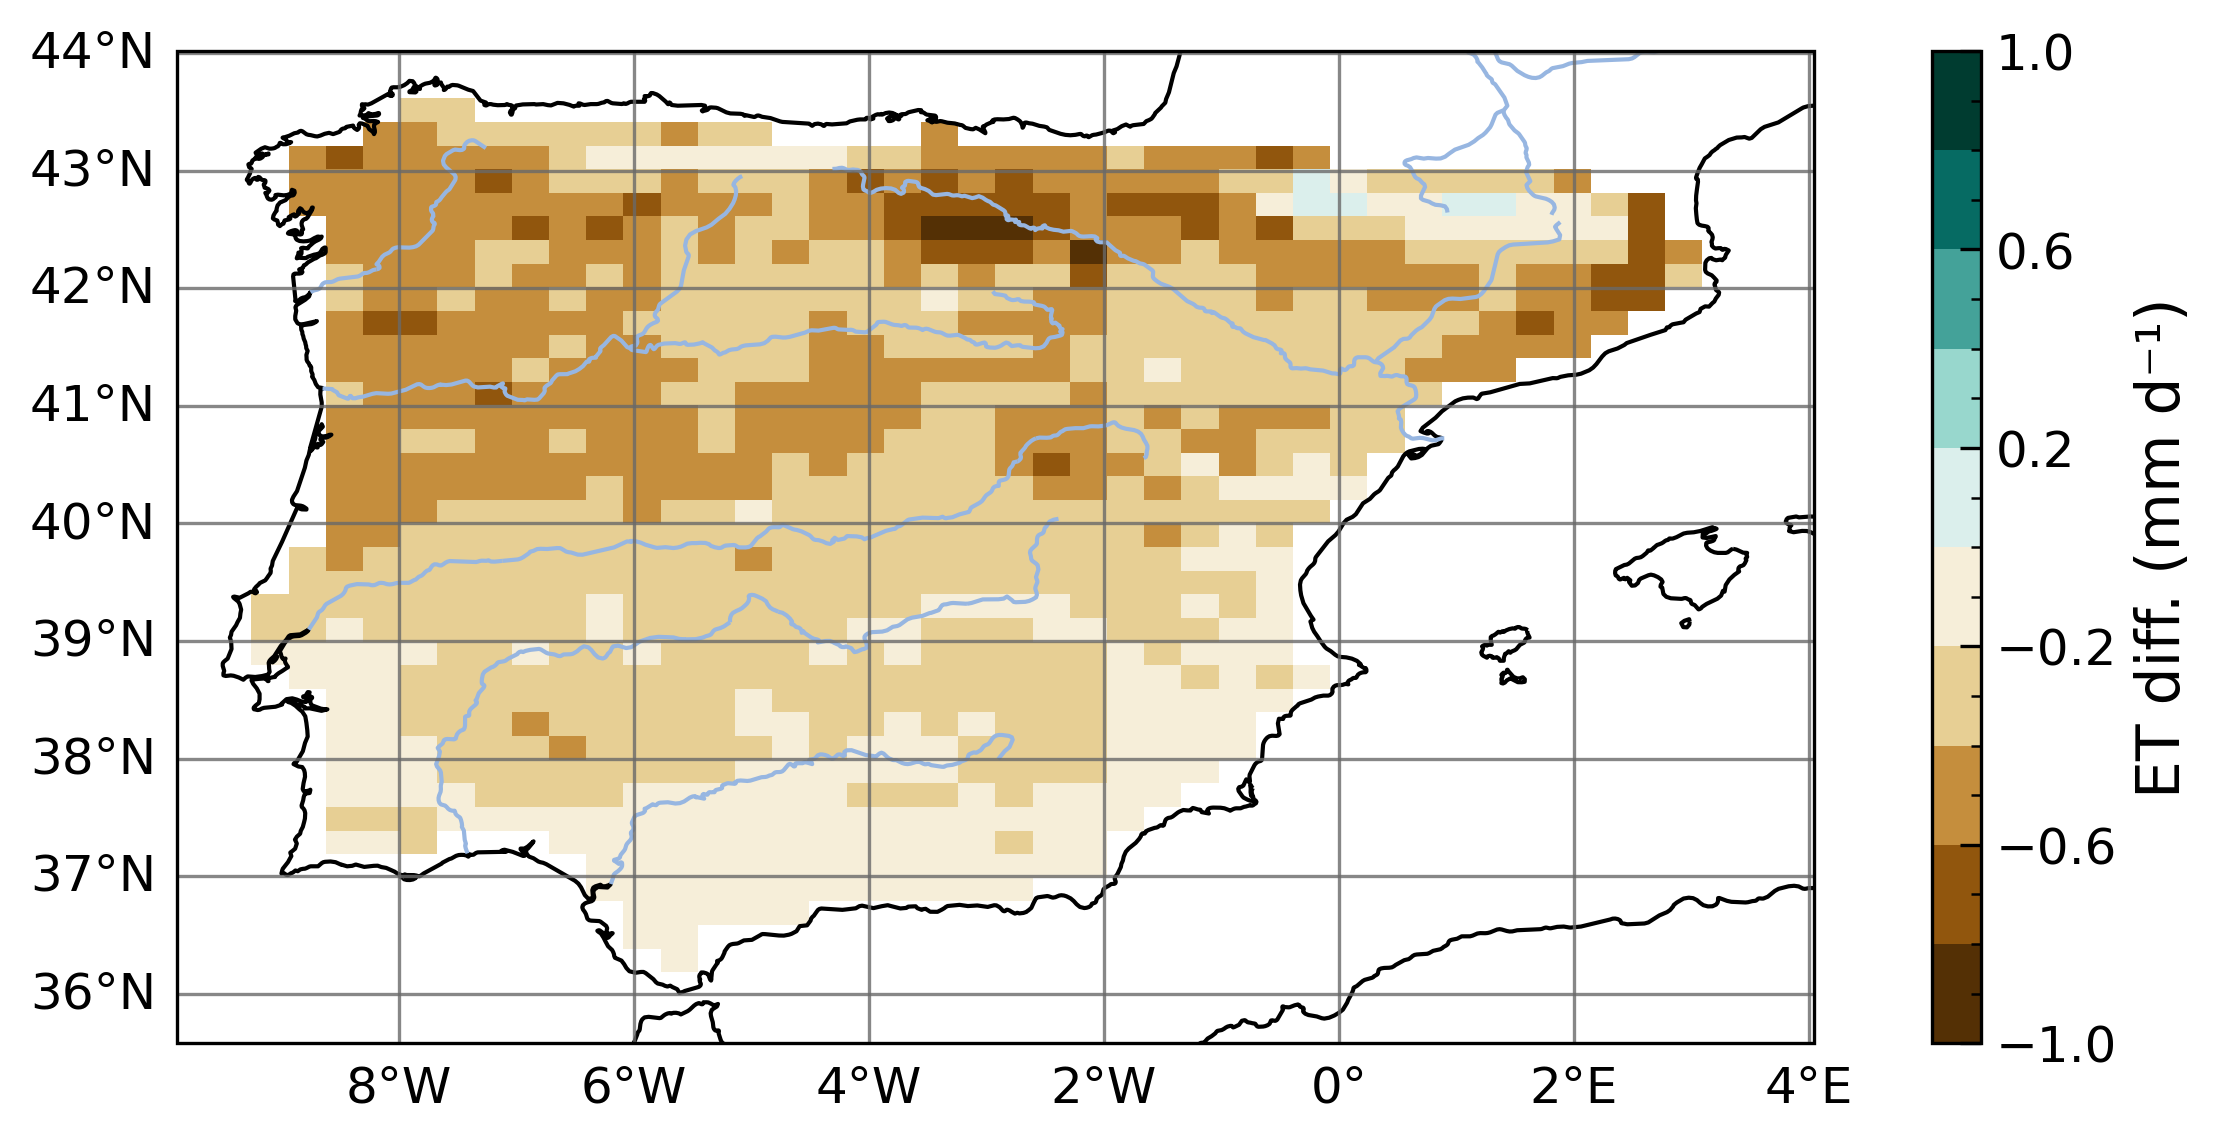
\includegraphics[width=\textwidth]{images/chap4/future/diffmap_JJA_evap_presfut.png}
        \end{subfigure} \\

        %t2m
        \begin{subfigure}[b]{0.5\textwidth}
            \caption{}
            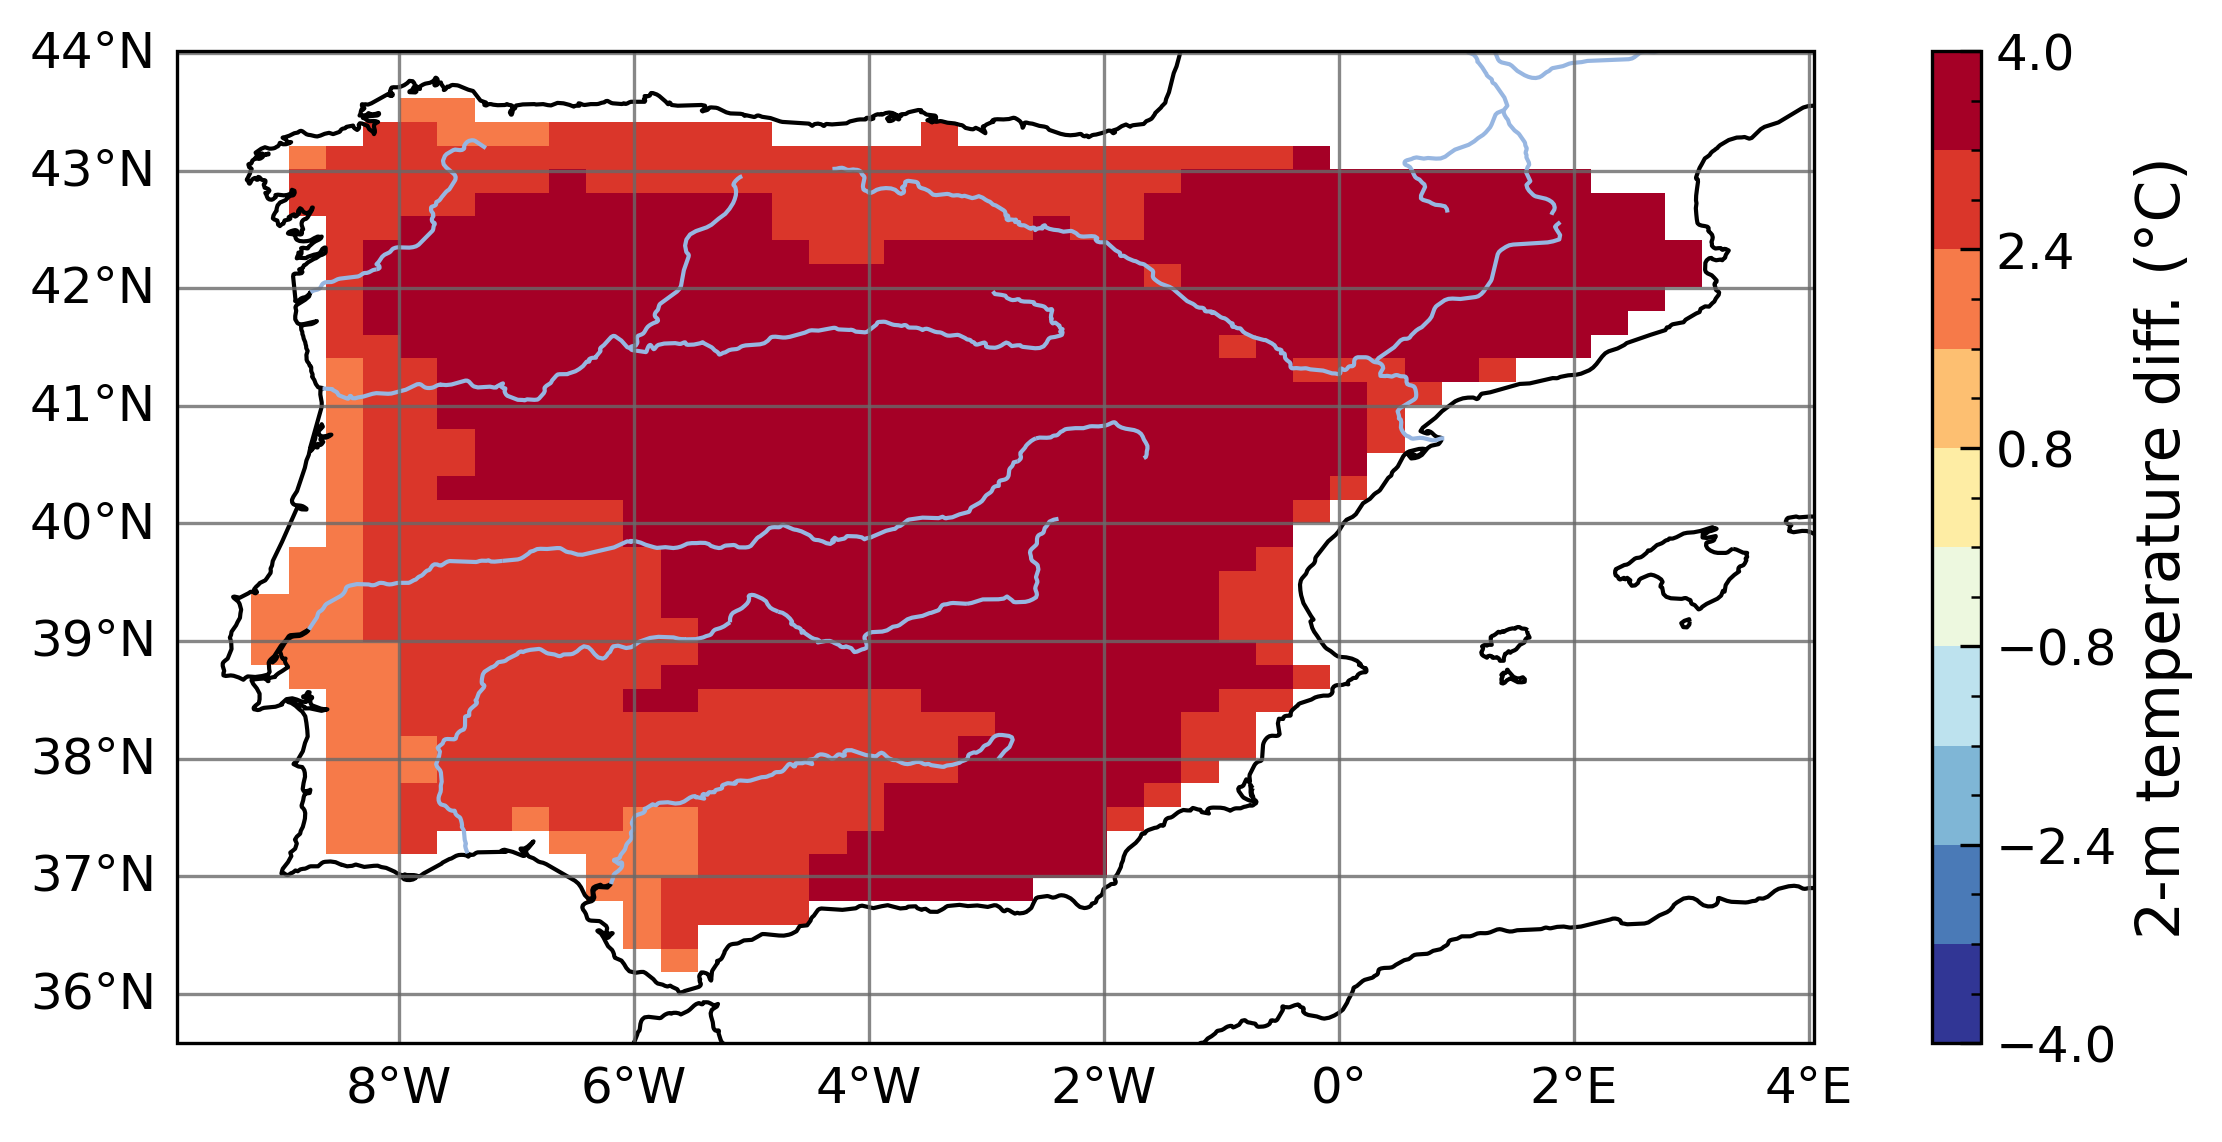
\includegraphics[width=\textwidth]{images/chap4/future/diffmap_JJA_t2m_presfut.png}
        \end{subfigure} &
        %fluxsens
        \begin{subfigure}[b]{0.5\textwidth}
            \caption{}
            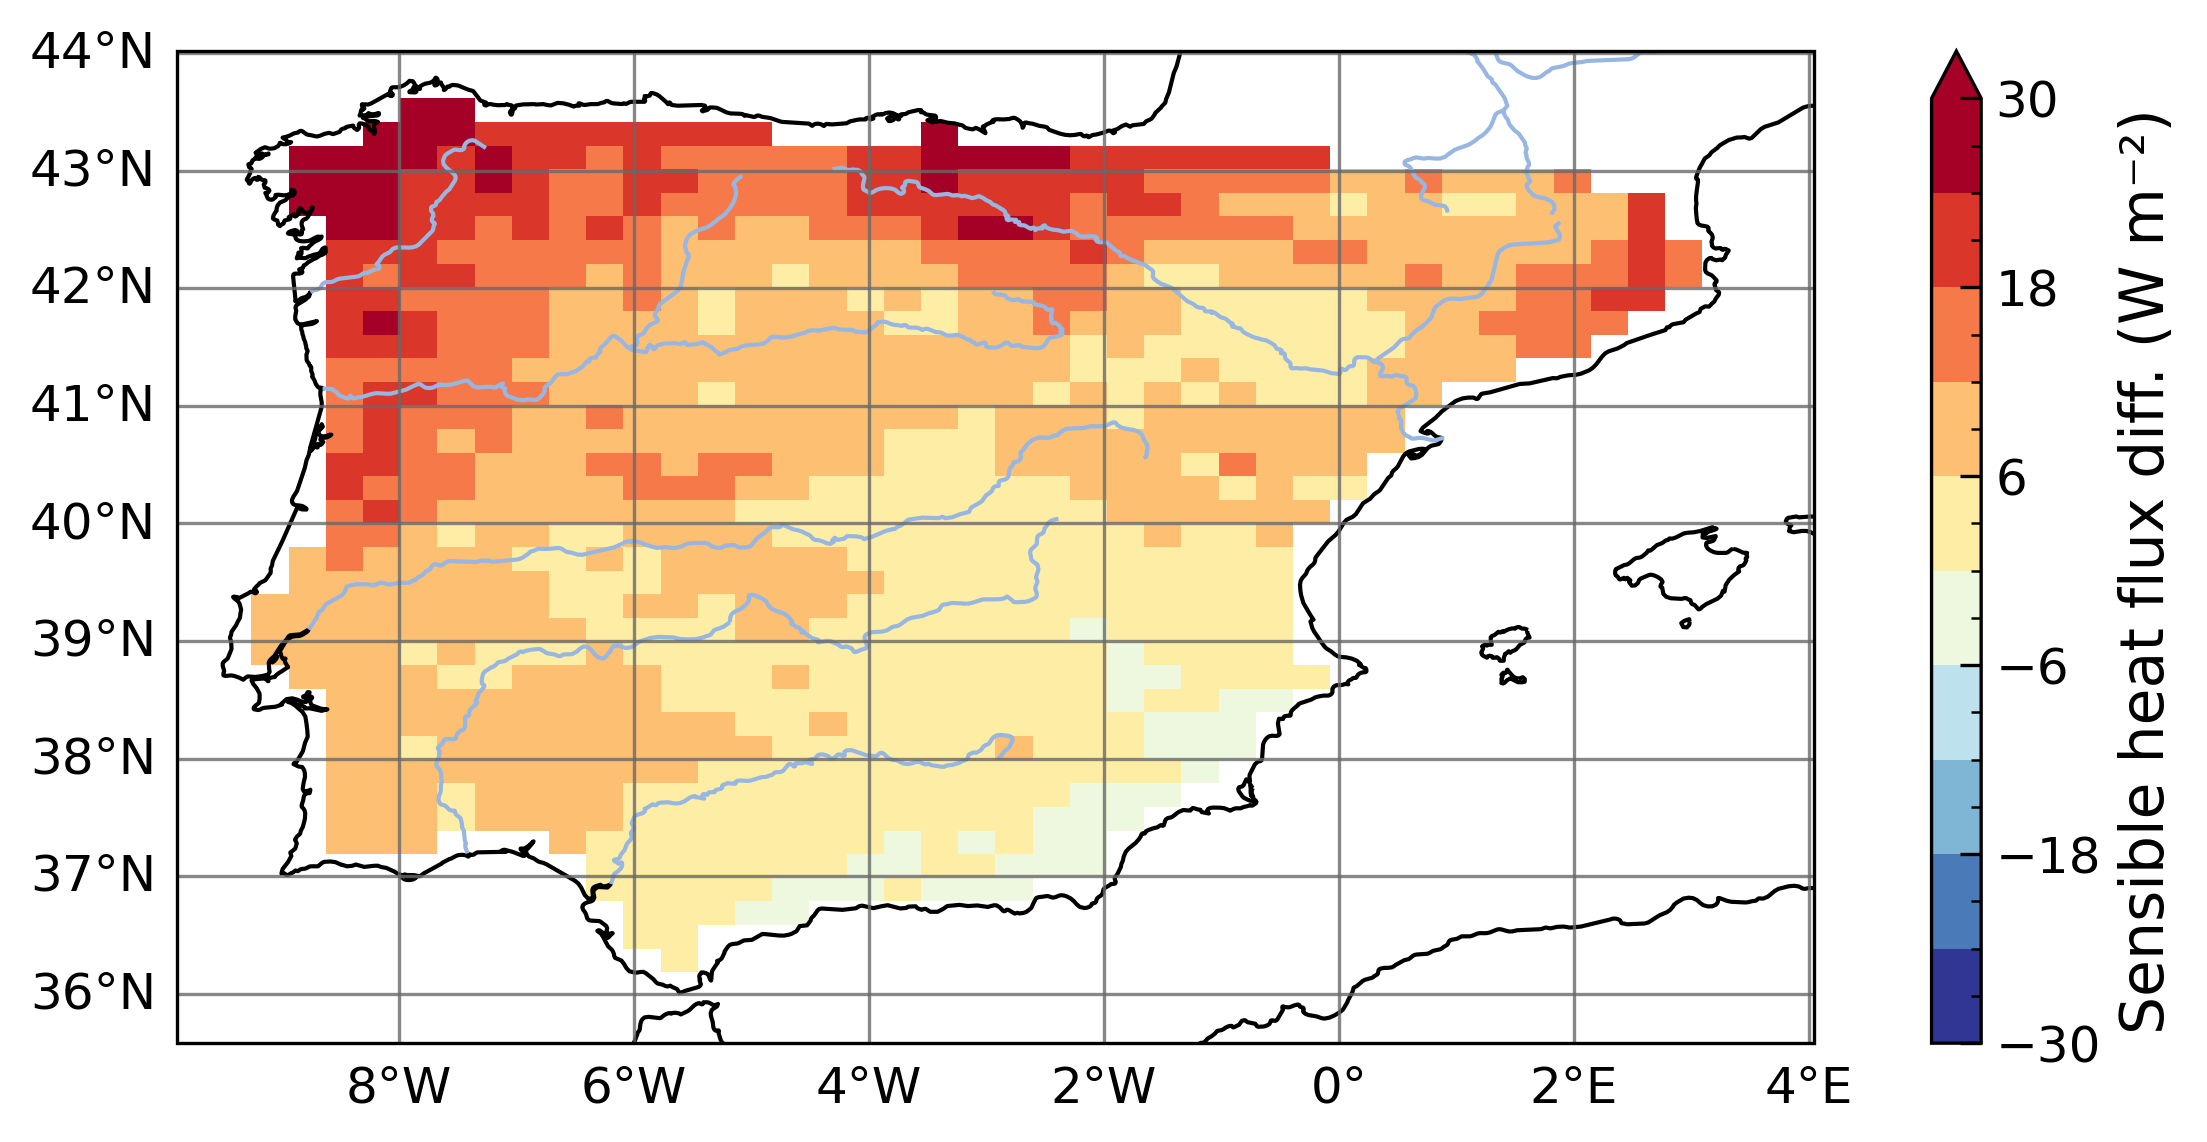
\includegraphics[width=\textwidth]{images/chap4/future/diffmap_JJA_fluxsens_presfut.png}
        \end{subfigure} \\

        %q2m
        \begin{subfigure}[b]{0.5\textwidth}
            \caption{}
            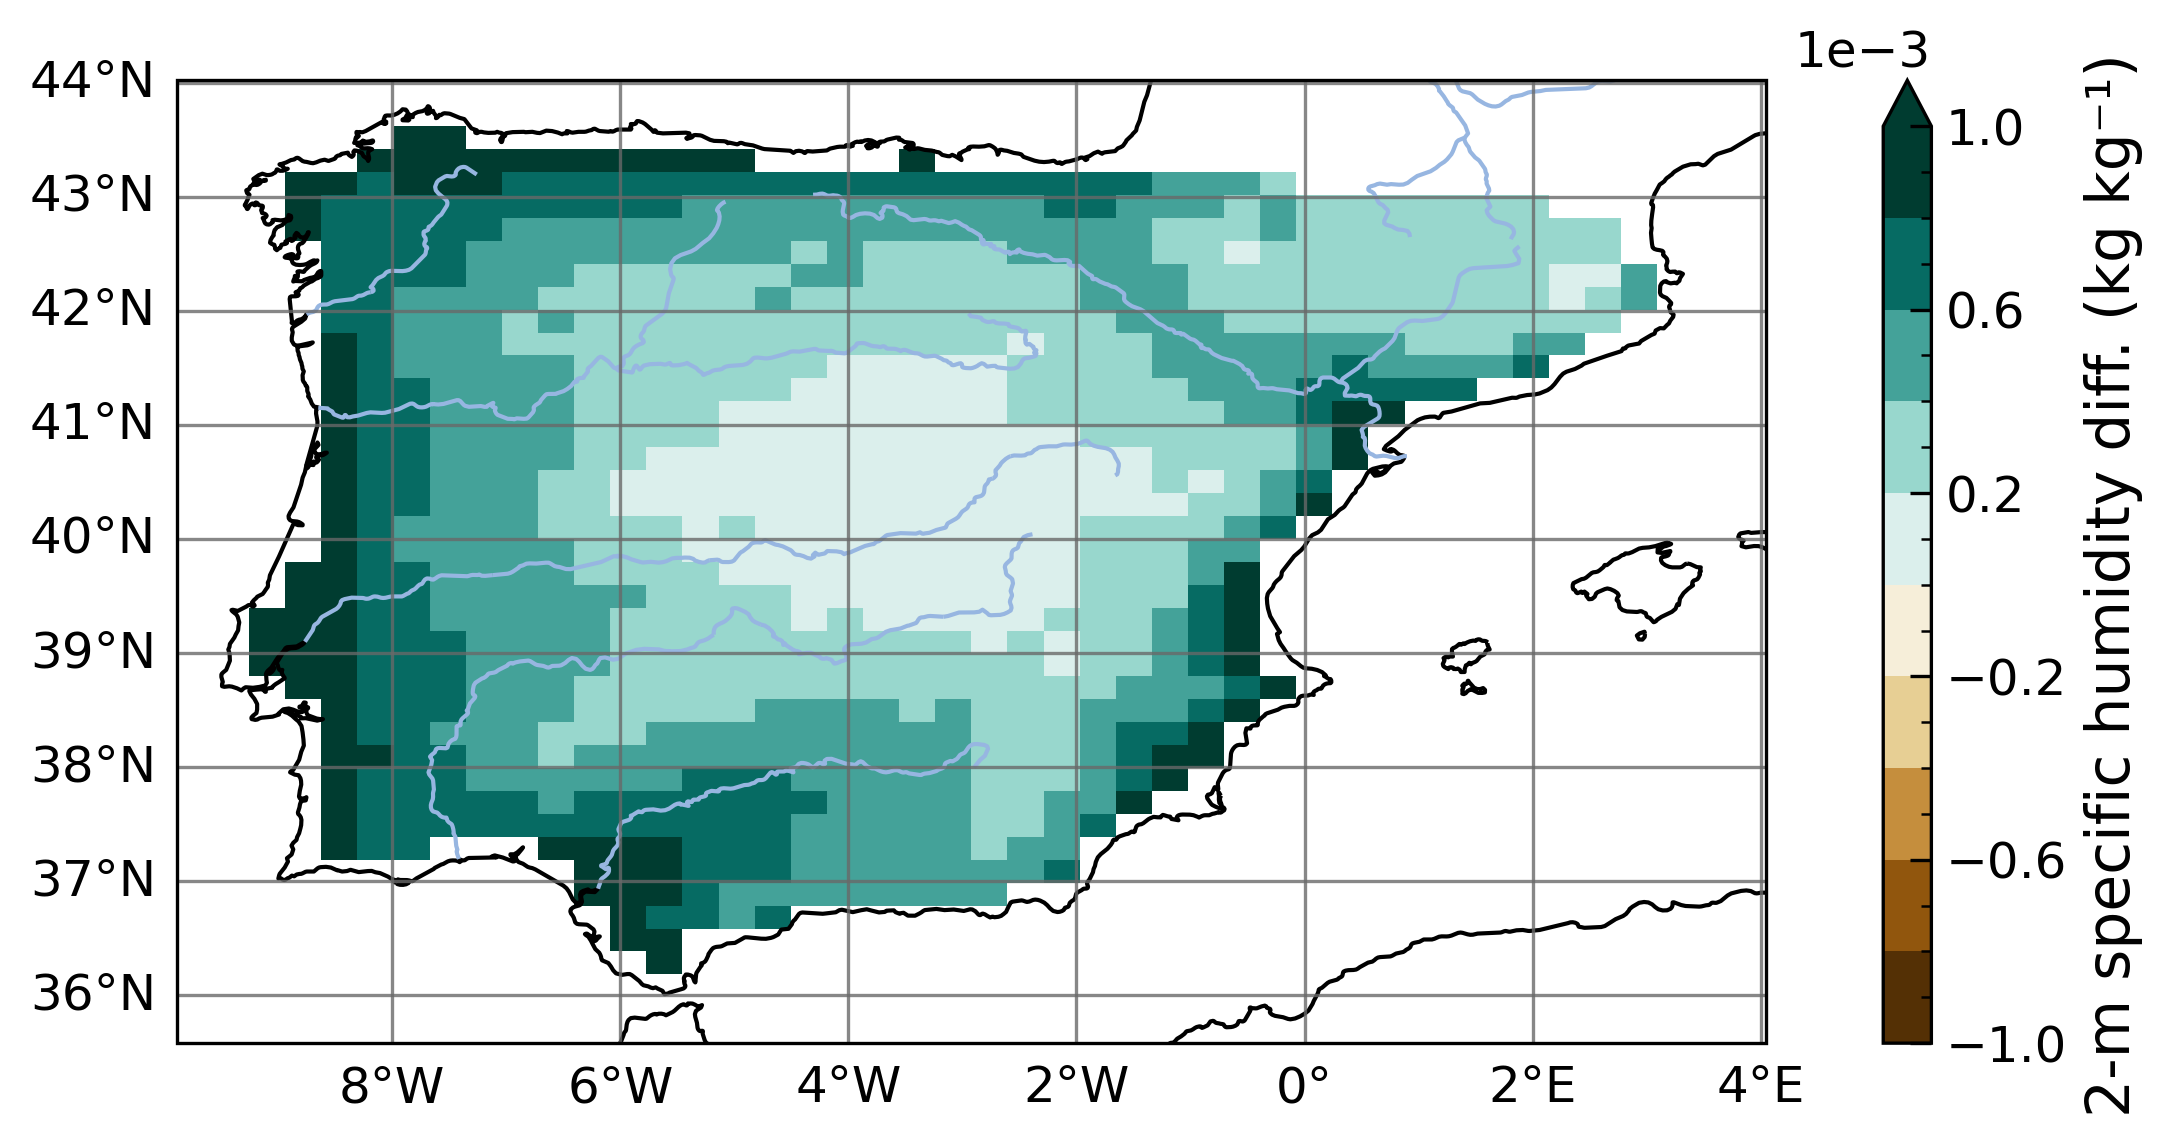
\includegraphics[width=\textwidth]{images/chap4/future/diffmap_JJA_q2m_presfut.png}
        \end{subfigure} &
        %rh2m
        \begin{subfigure}[b]{0.5\textwidth}
            \caption{}
            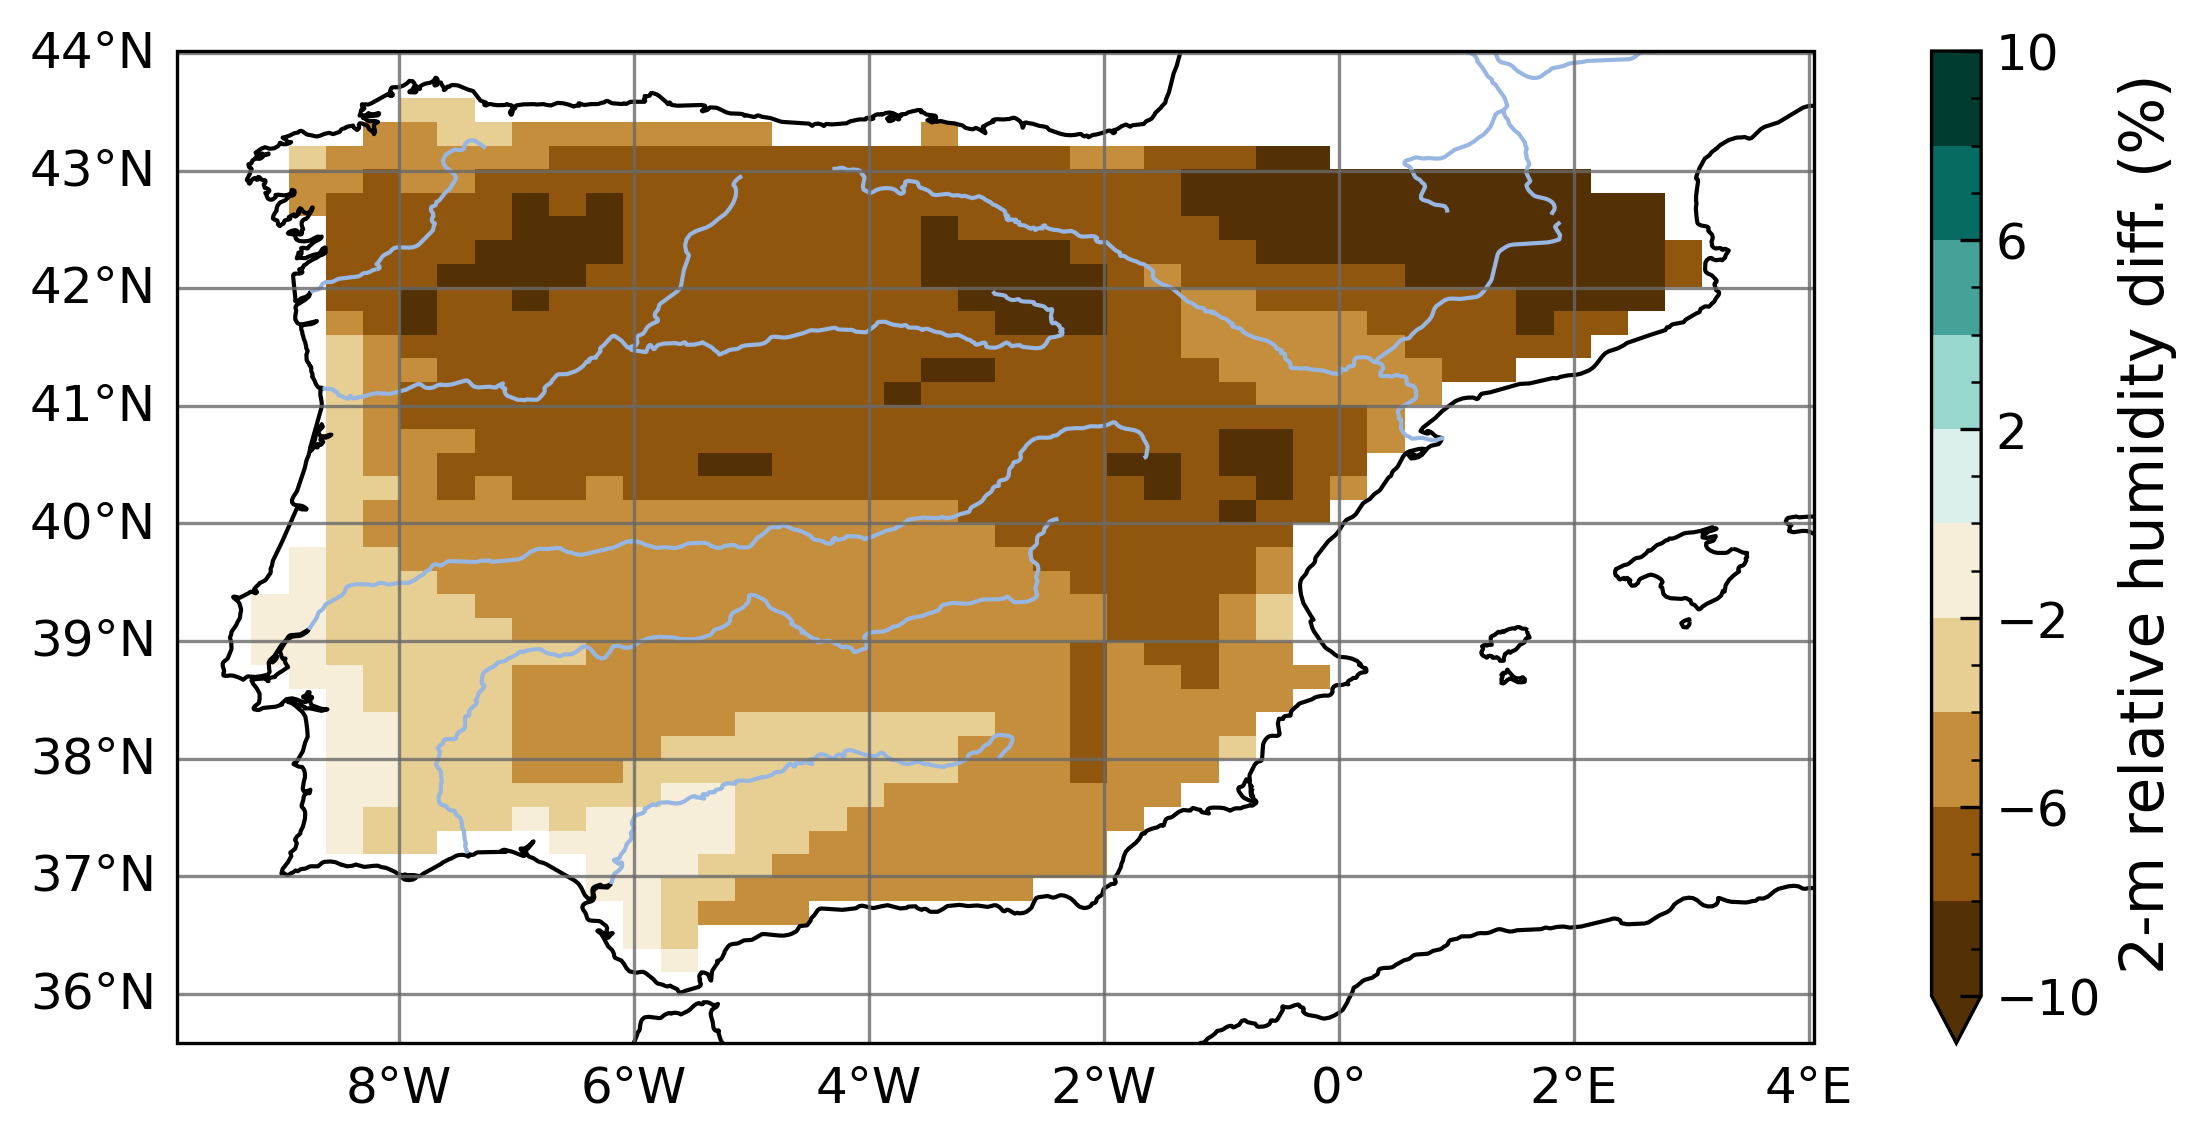
\includegraphics[width=\textwidth]{images/chap4/future/diffmap_JJA_rh2m_presfut.png}
        \end{subfigure} \\

        %pblh
        \begin{subfigure}[b]{0.5\textwidth}
            \caption{}
            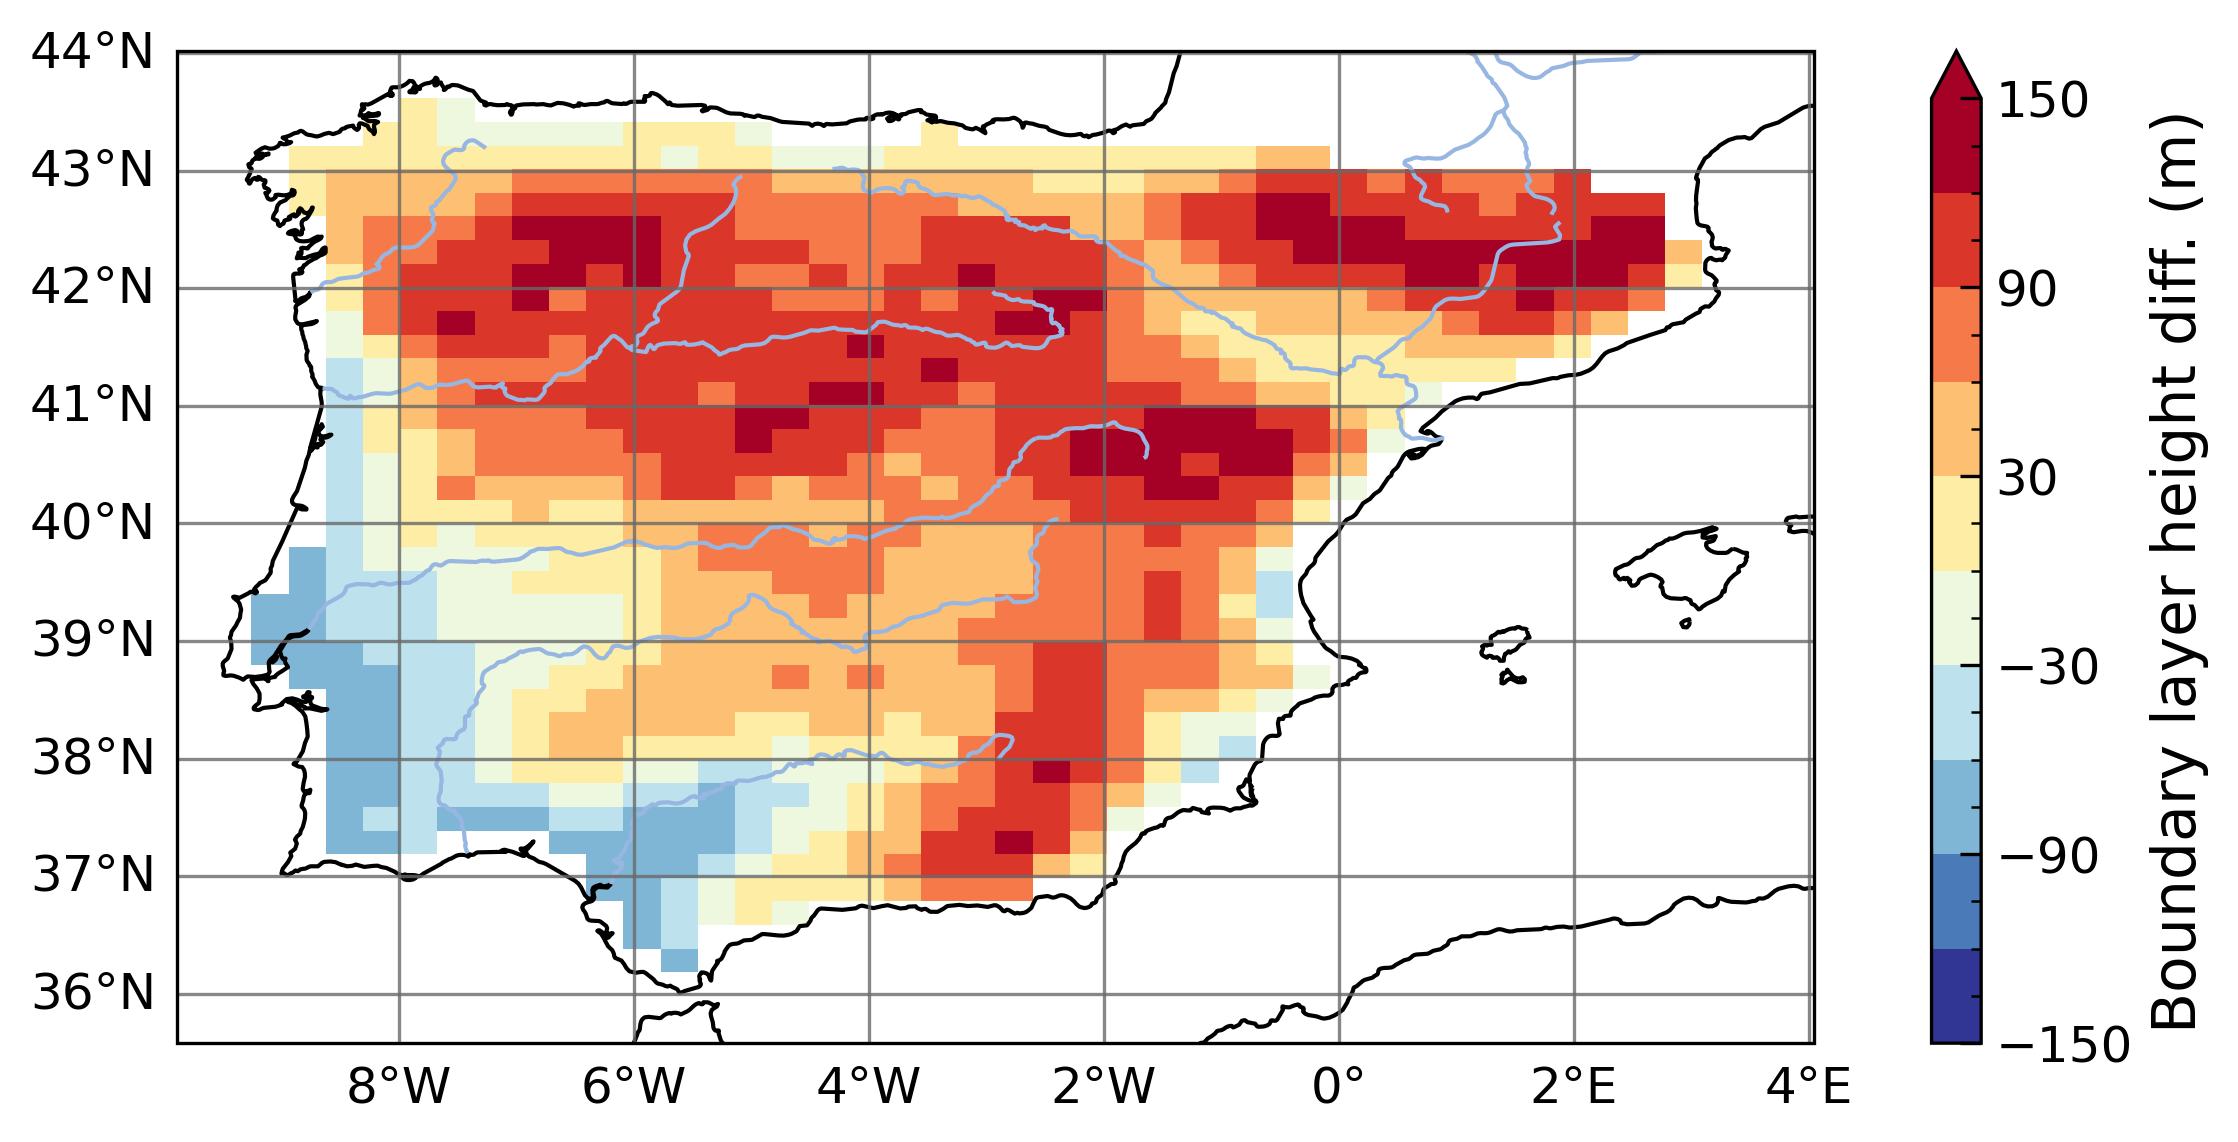
\includegraphics[width=\textwidth]{images/chap4/future/diffmap_JJA_s_pblh_presfut.png}
        \end{subfigure} &
        %lcl
        \begin{subfigure}[b]{0.5\textwidth}
            \caption{}
            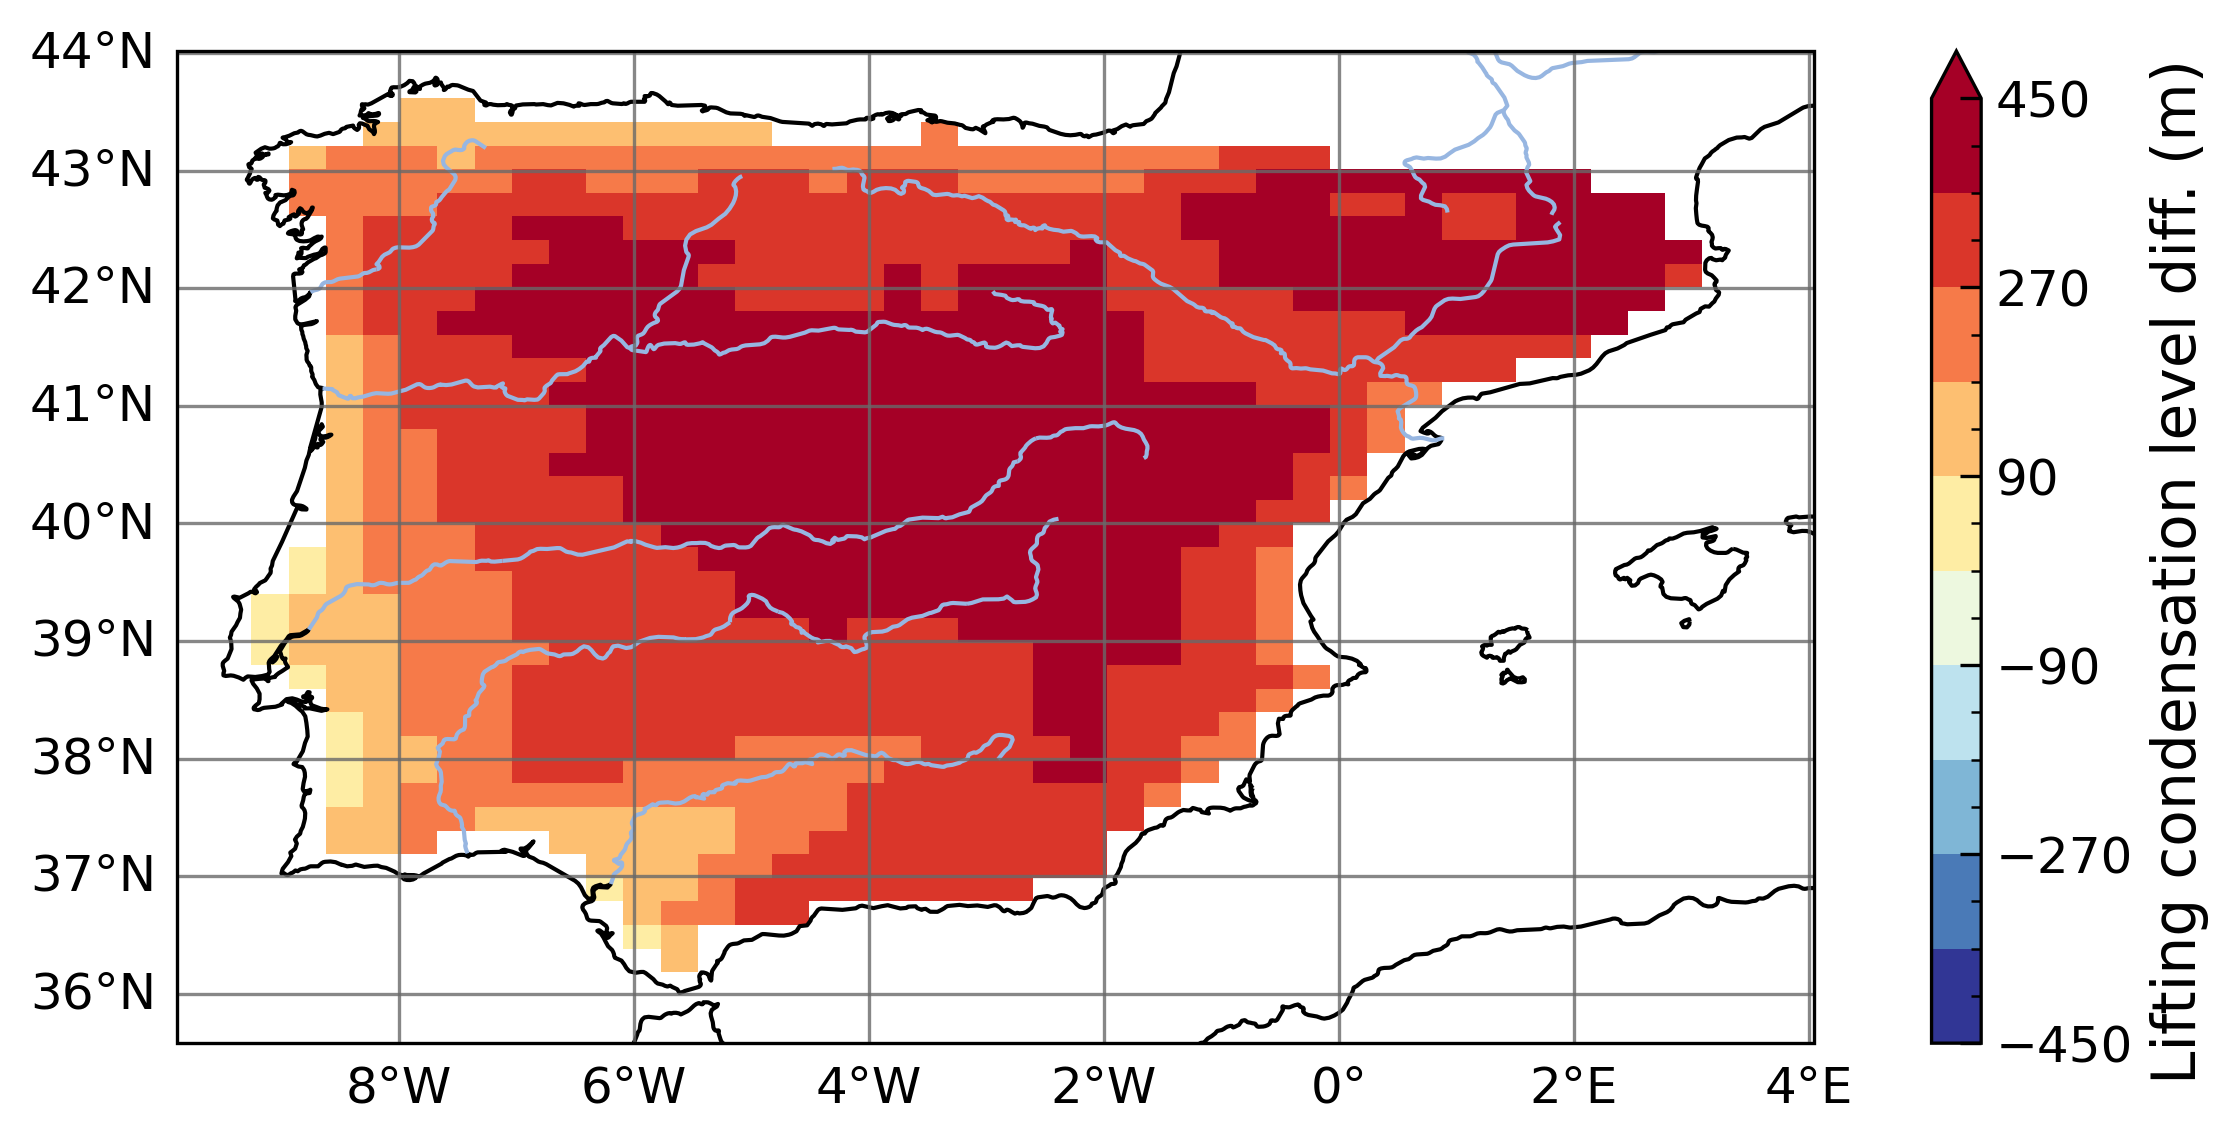
\includegraphics[width=\textwidth]{images/chap4/future/diffmap_JJA_s_lcl_presfut.png}
        \end{subfigure} \\
    \end{tabular}
    \caption{JJA}
    \label{fig:diffmaps_JJA_present_future}
\end{figure}


%figure : diff maps JJA (future, irr - no_irr)
\begin{figure}[htbp]
    \centering
    \begin{tabular}{cc}
        %precip
        \begin{subfigure}[b]{0.5\textwidth}
            \caption{}
            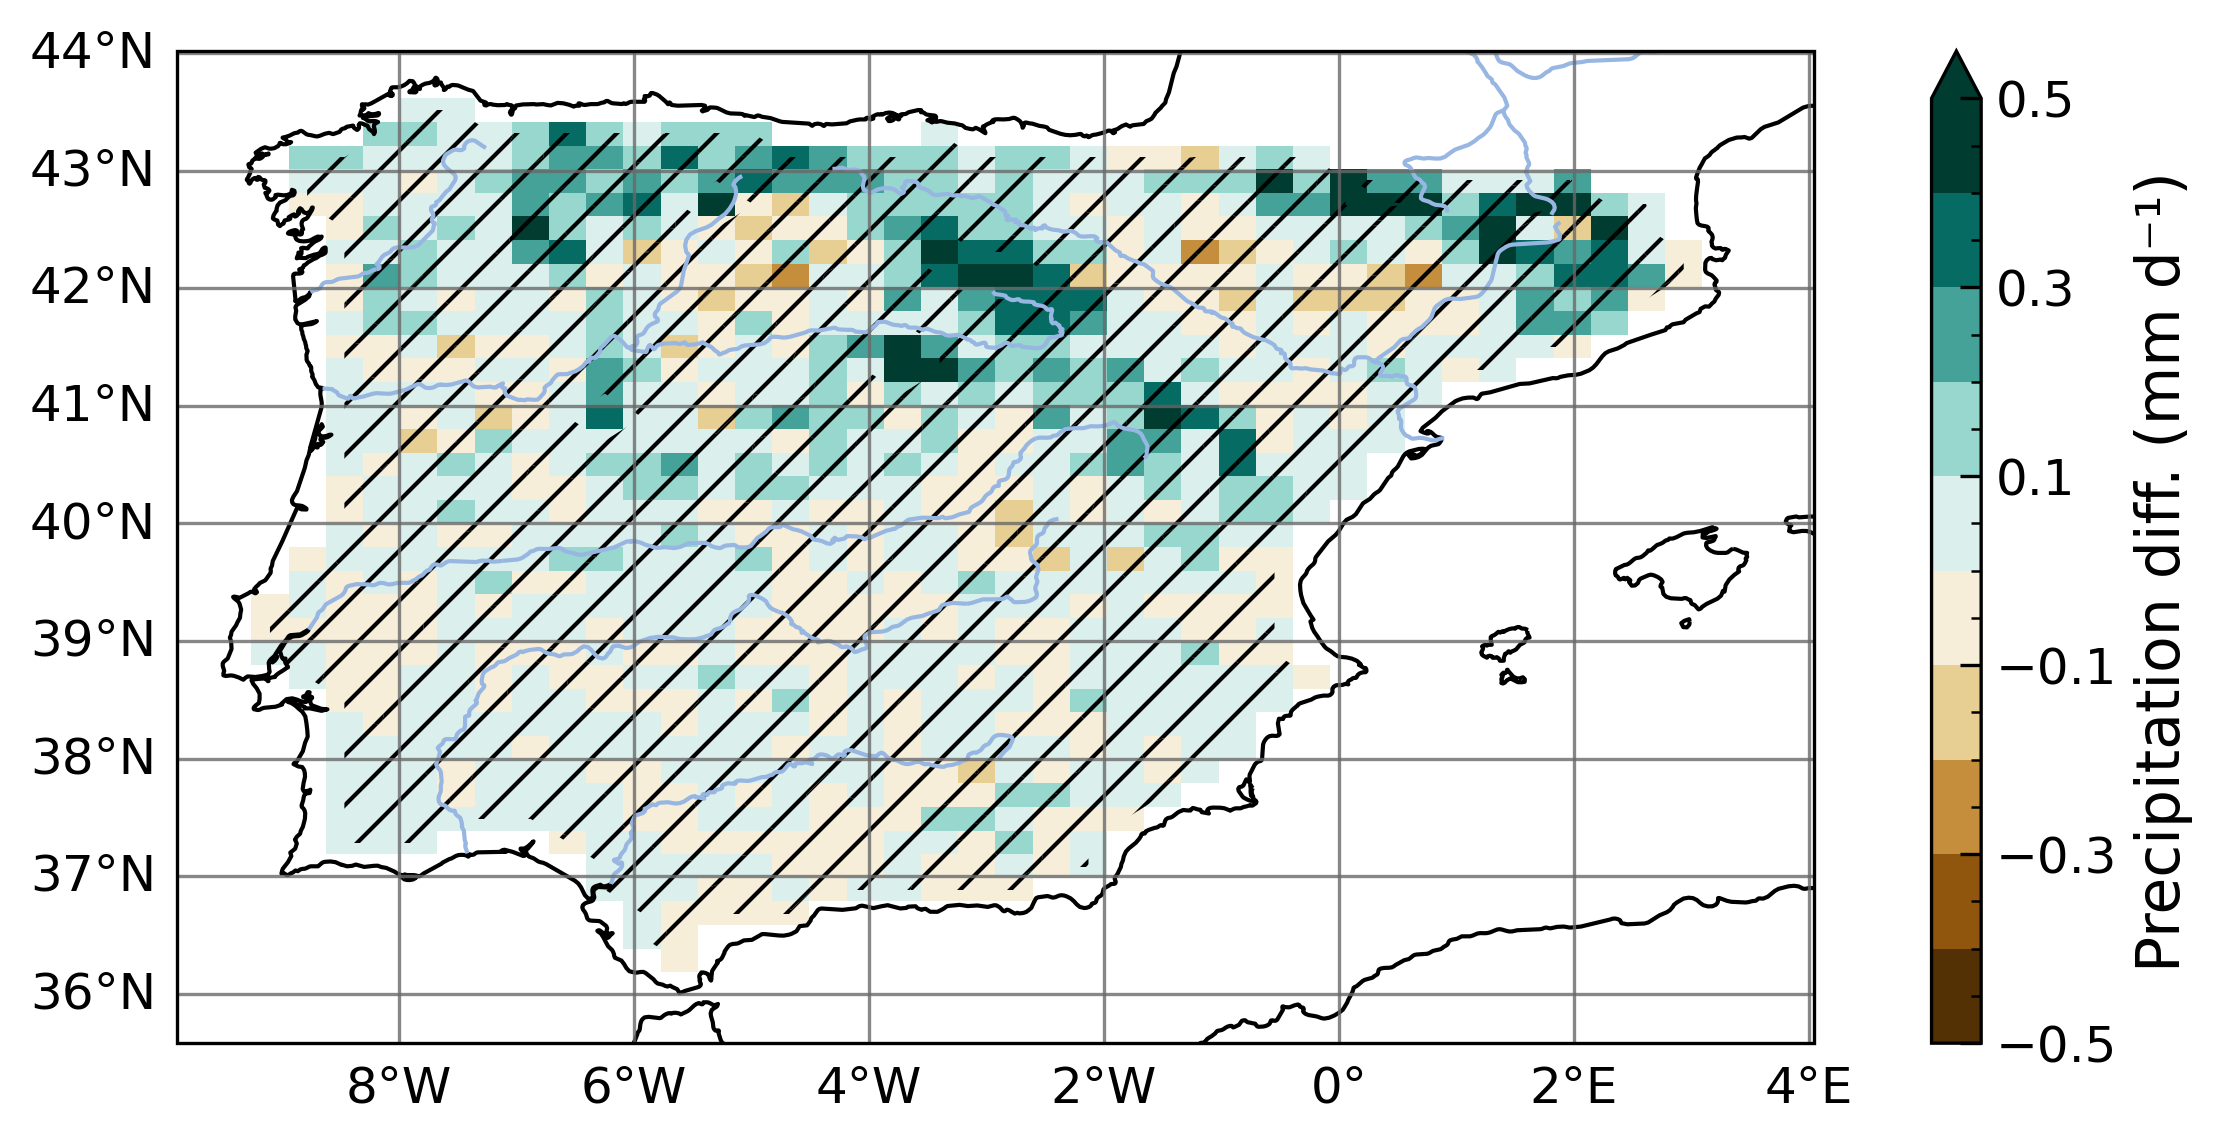
\includegraphics[width=\textwidth]{images/chap4/future/diffmap_JJA_precip_futirr.png}
        \end{subfigure} &
        %evap
        \begin{subfigure}[b]{0.5\textwidth}
            \caption{}
            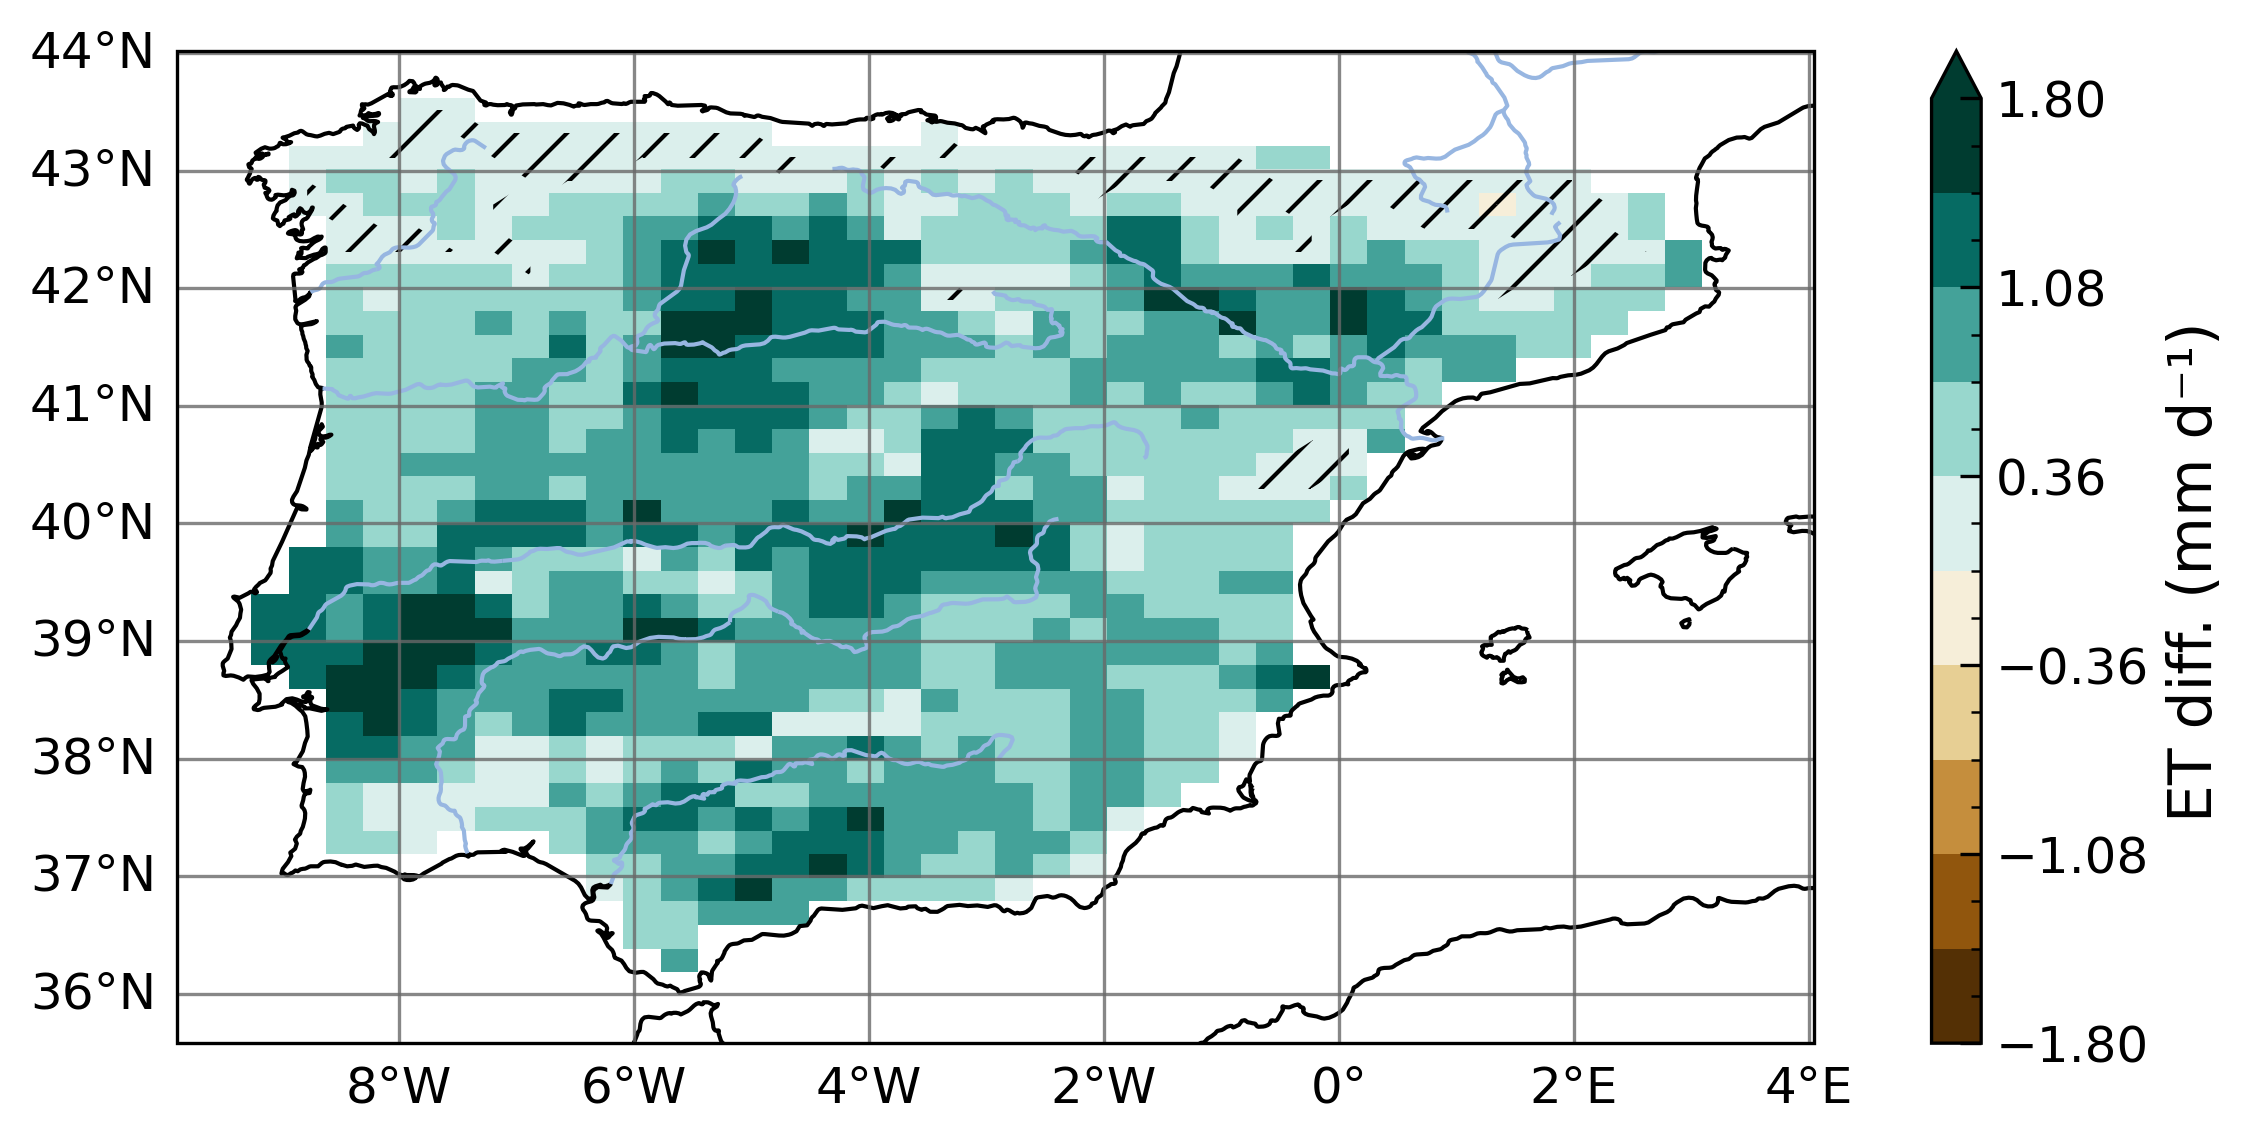
\includegraphics[width=\textwidth]{images/chap4/future/diffmap_JJA_evap_futirr.png}
        \end{subfigure} \\

        %t2m
        \begin{subfigure}[b]{0.5\textwidth}
            \caption{}
            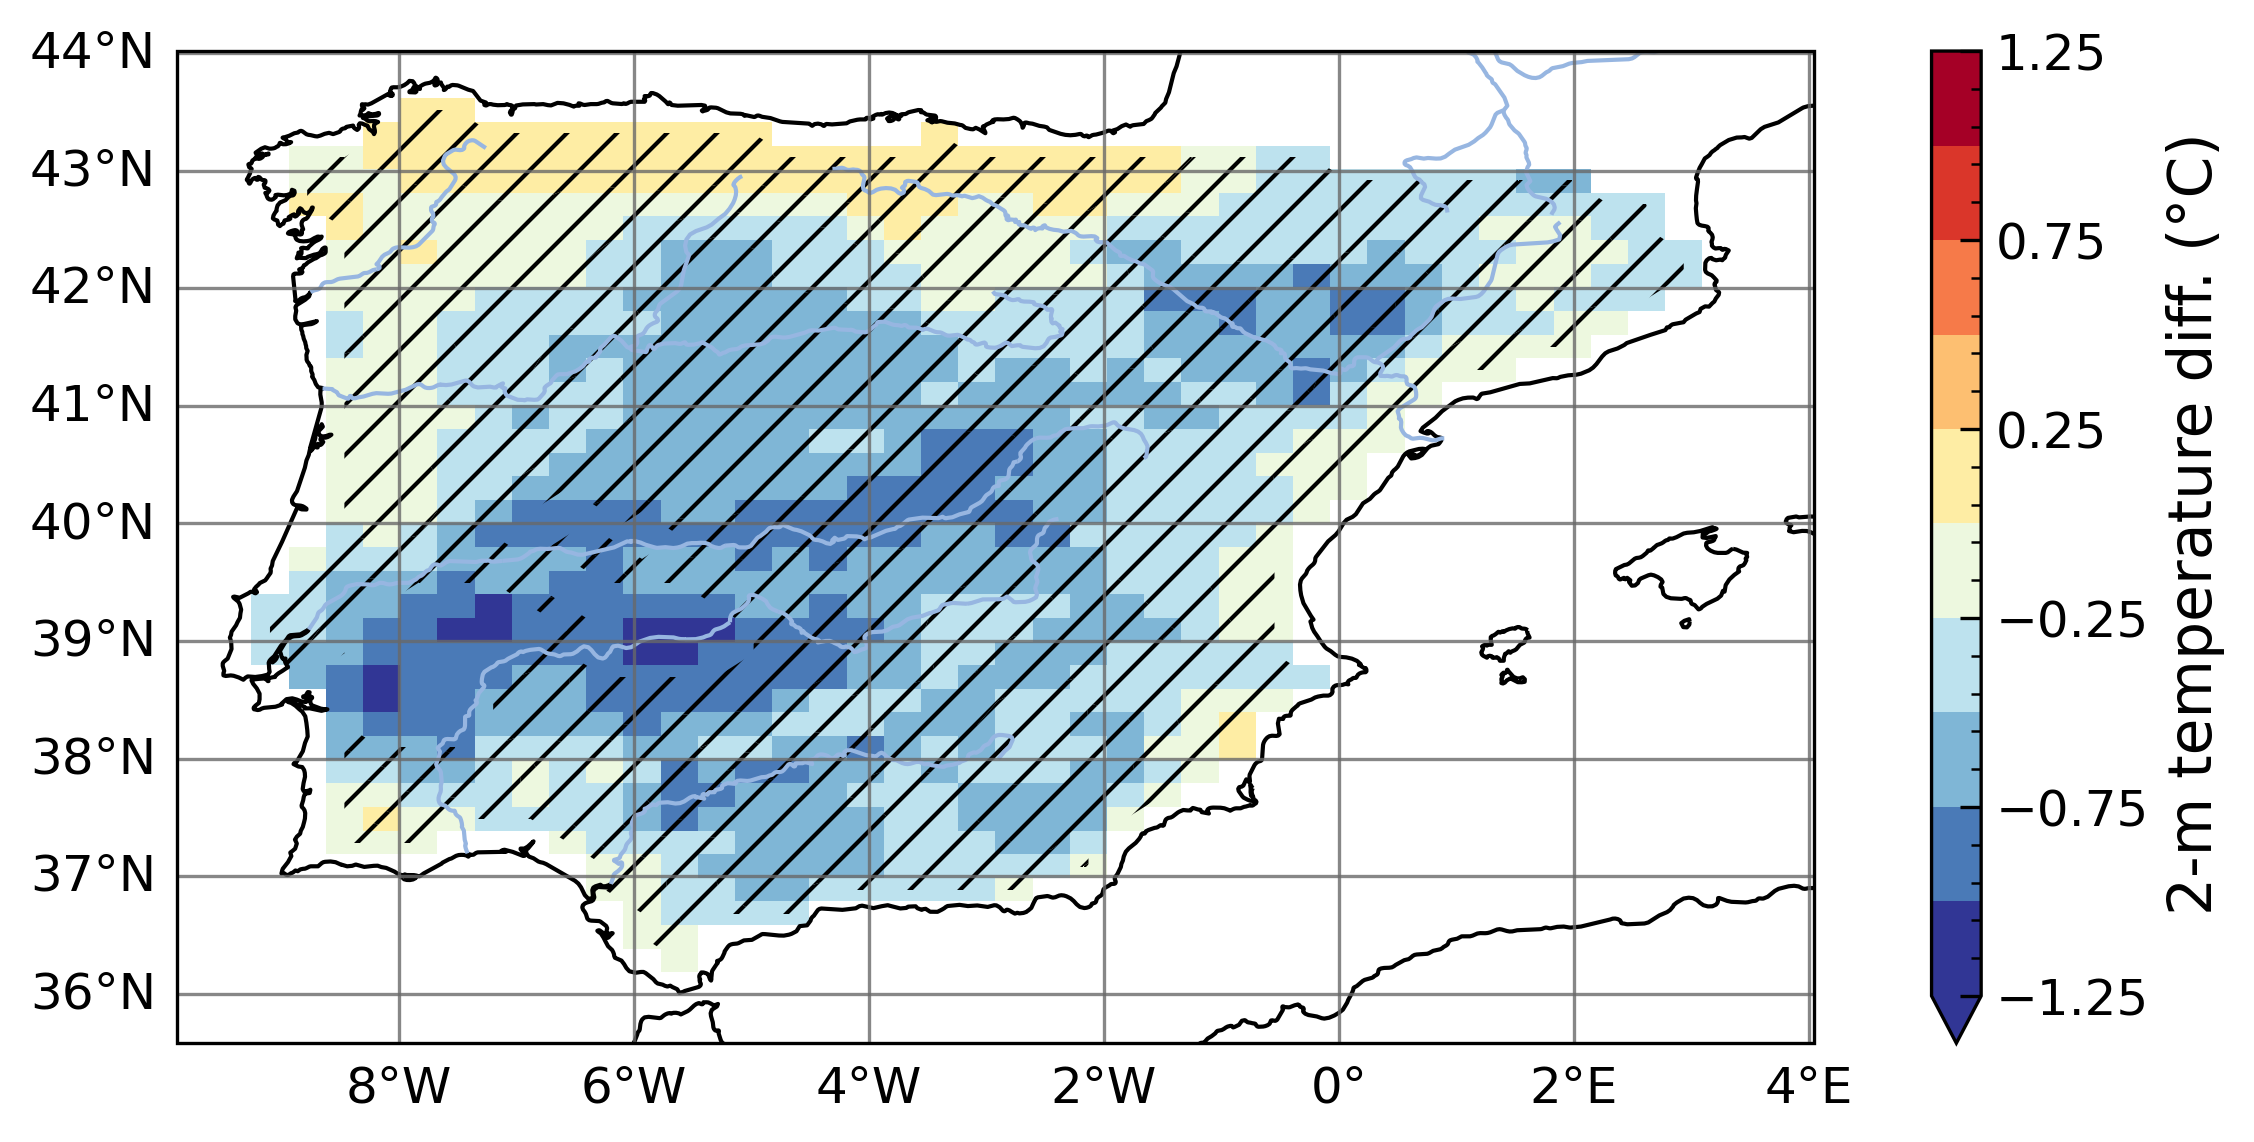
\includegraphics[width=\textwidth]{images/chap4/future/diffmap_JJA_t2m_futirr.png}
        \end{subfigure} &
        %fluxsens
        \begin{subfigure}[b]{0.5\textwidth}
            \caption{}
            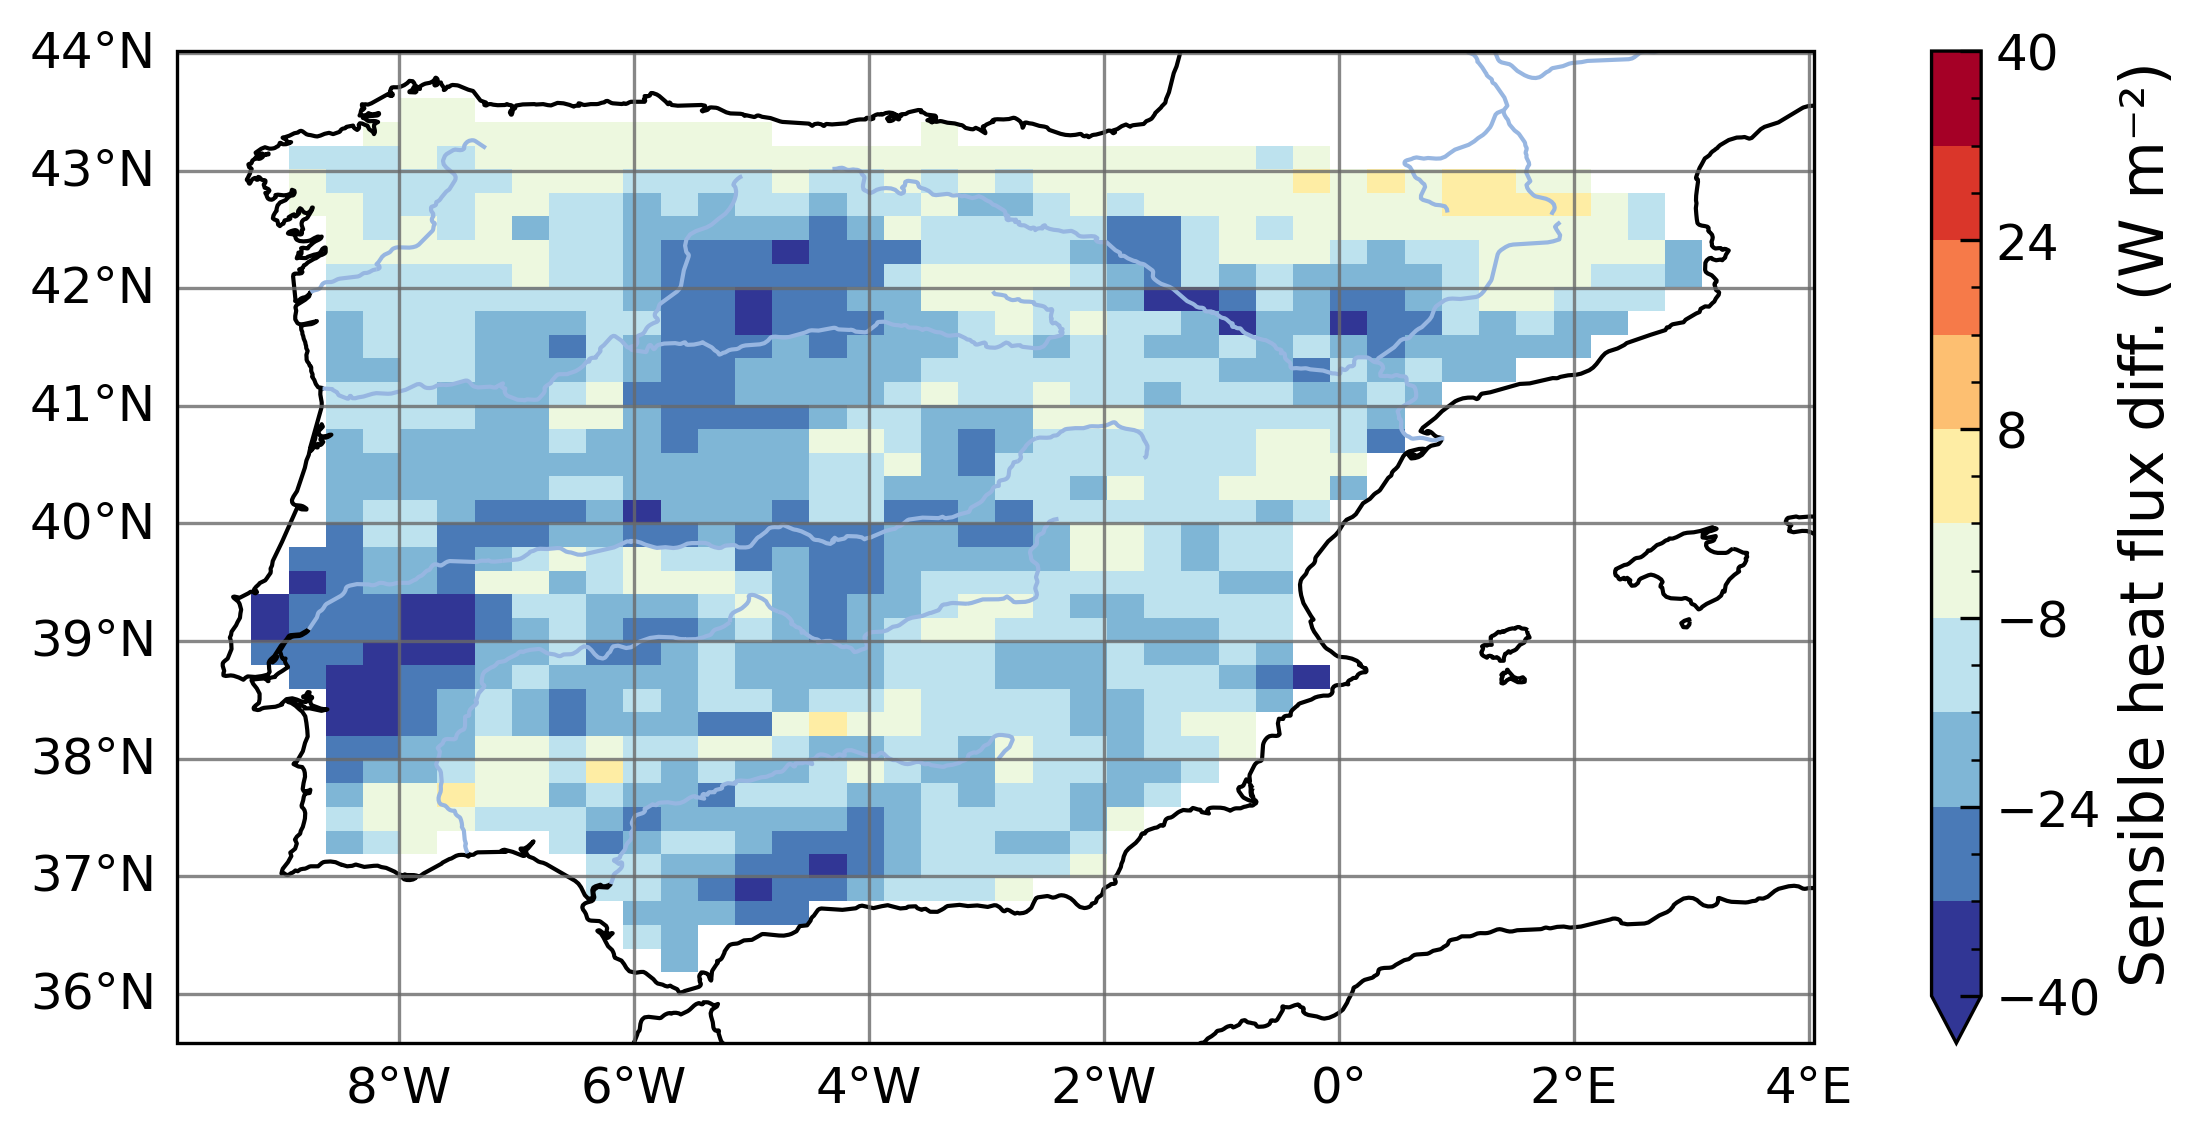
\includegraphics[width=\textwidth]{images/chap4/future/diffmap_JJA_fluxsens_futirr.png}
        \end{subfigure} \\

        %q2m
        \begin{subfigure}[b]{0.5\textwidth}
            \caption{}
            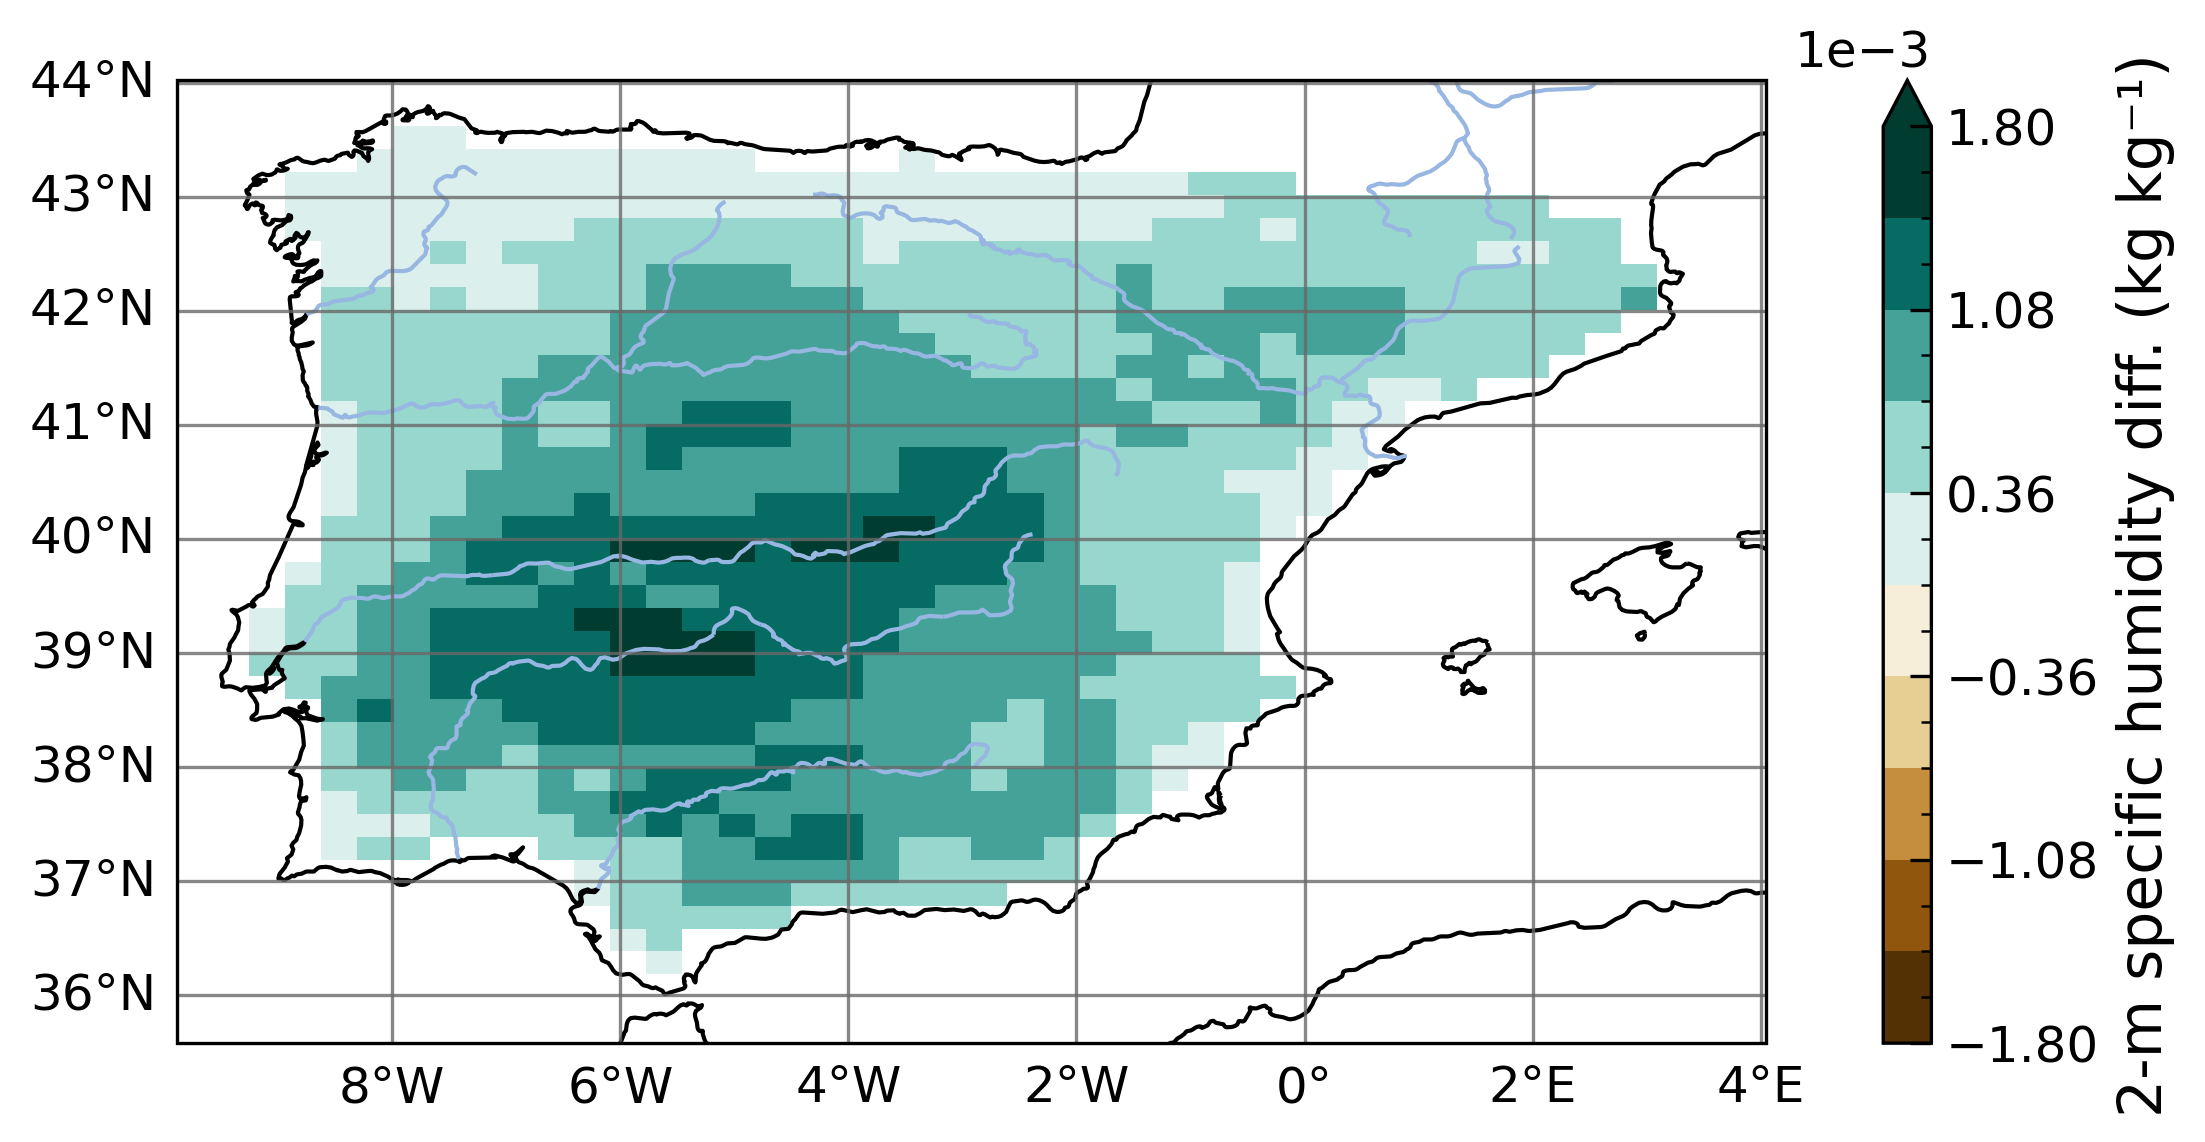
\includegraphics[width=\textwidth]{images/chap4/future/diffmap_JJA_q2m_futirr.png}
        \end{subfigure} &
        %rh2m
        \begin{subfigure}[b]{0.5\textwidth}
            \caption{}
            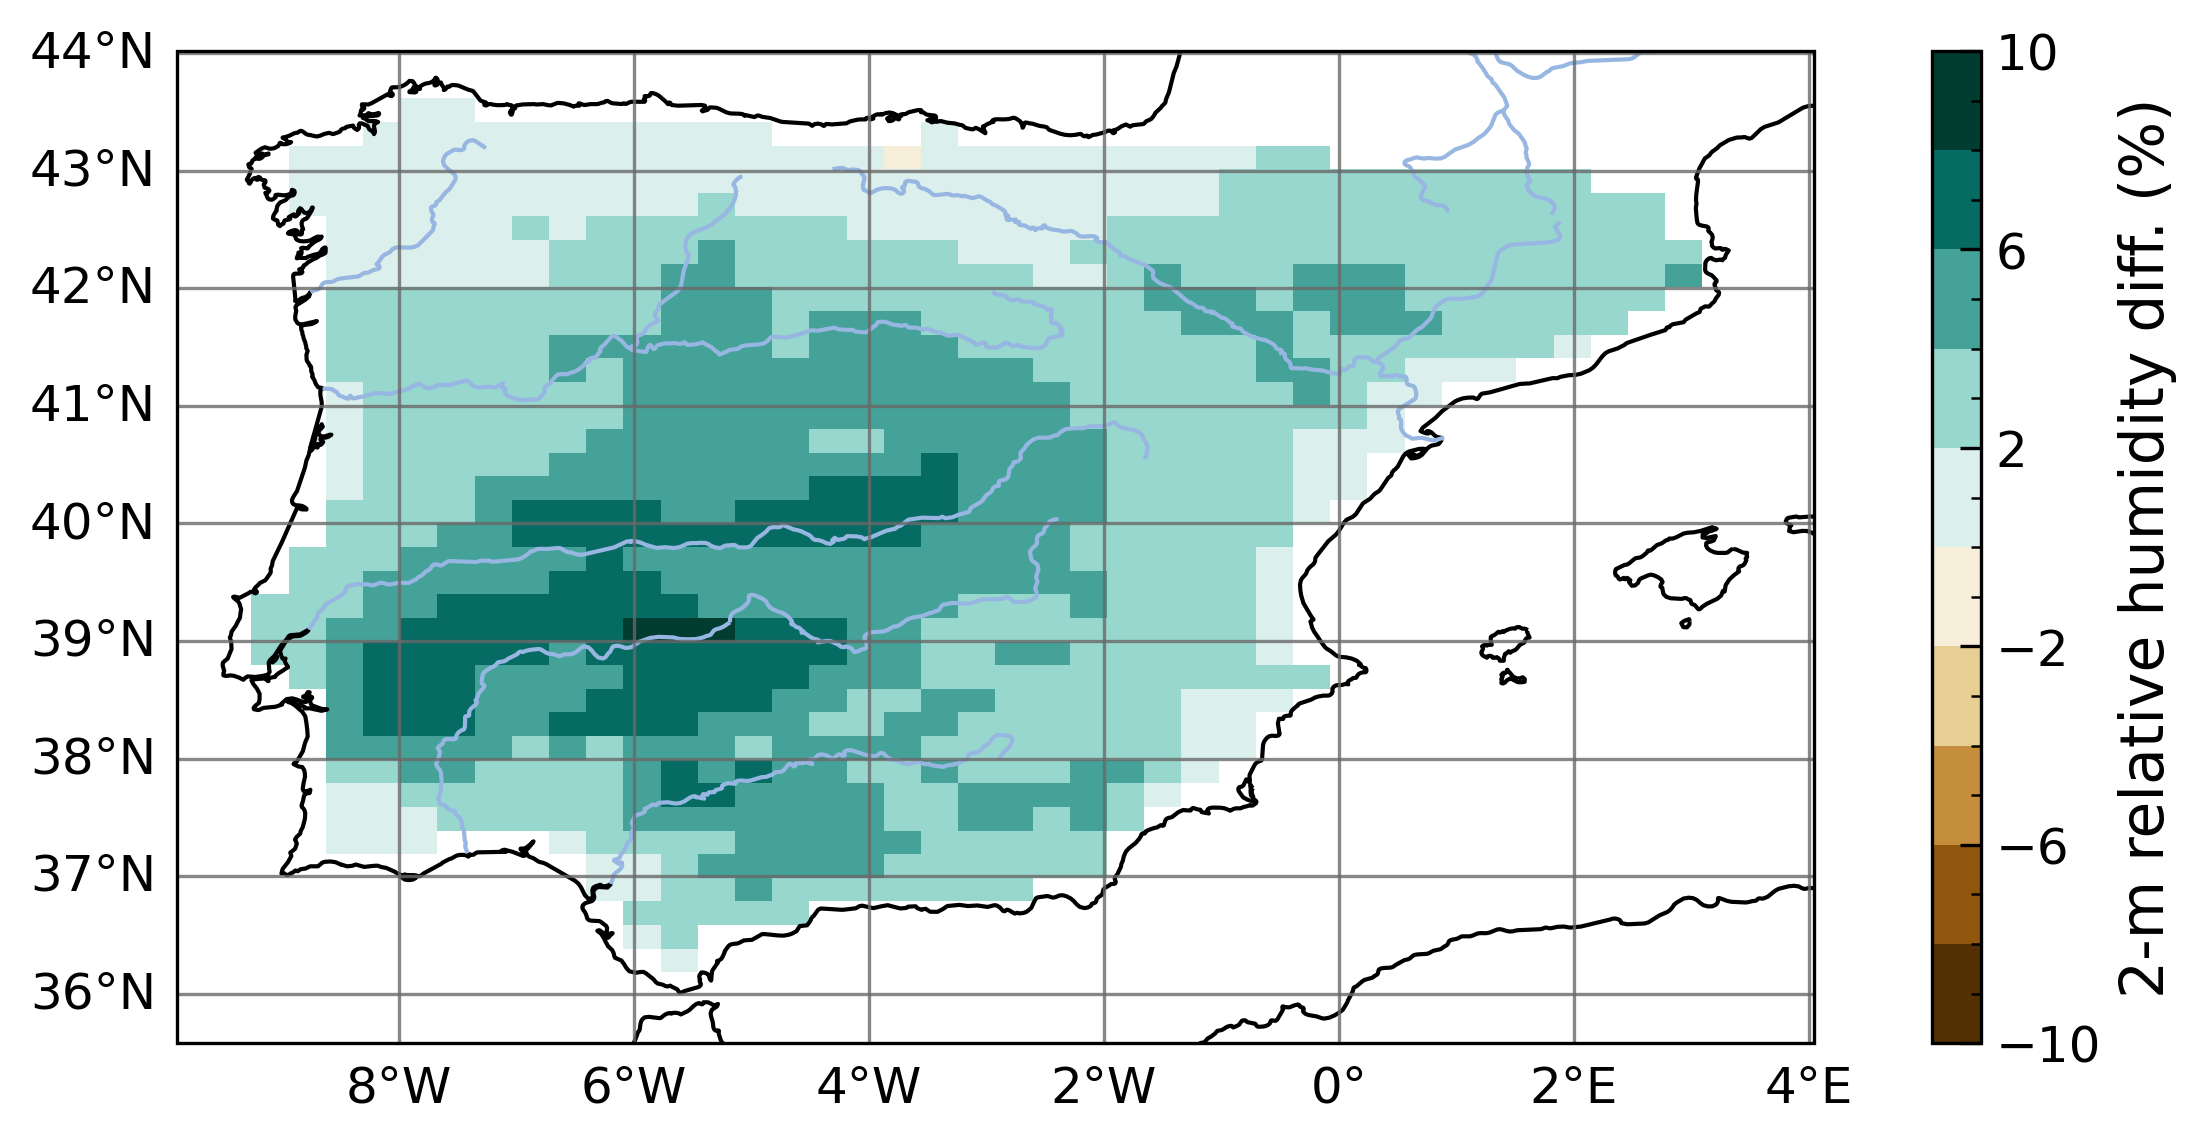
\includegraphics[width=\textwidth]{images/chap4/future/diffmap_JJA_rh2m_futirr.png}
        \end{subfigure} \\

        %pblh
        \begin{subfigure}[b]{0.5\textwidth}
            \caption{}
            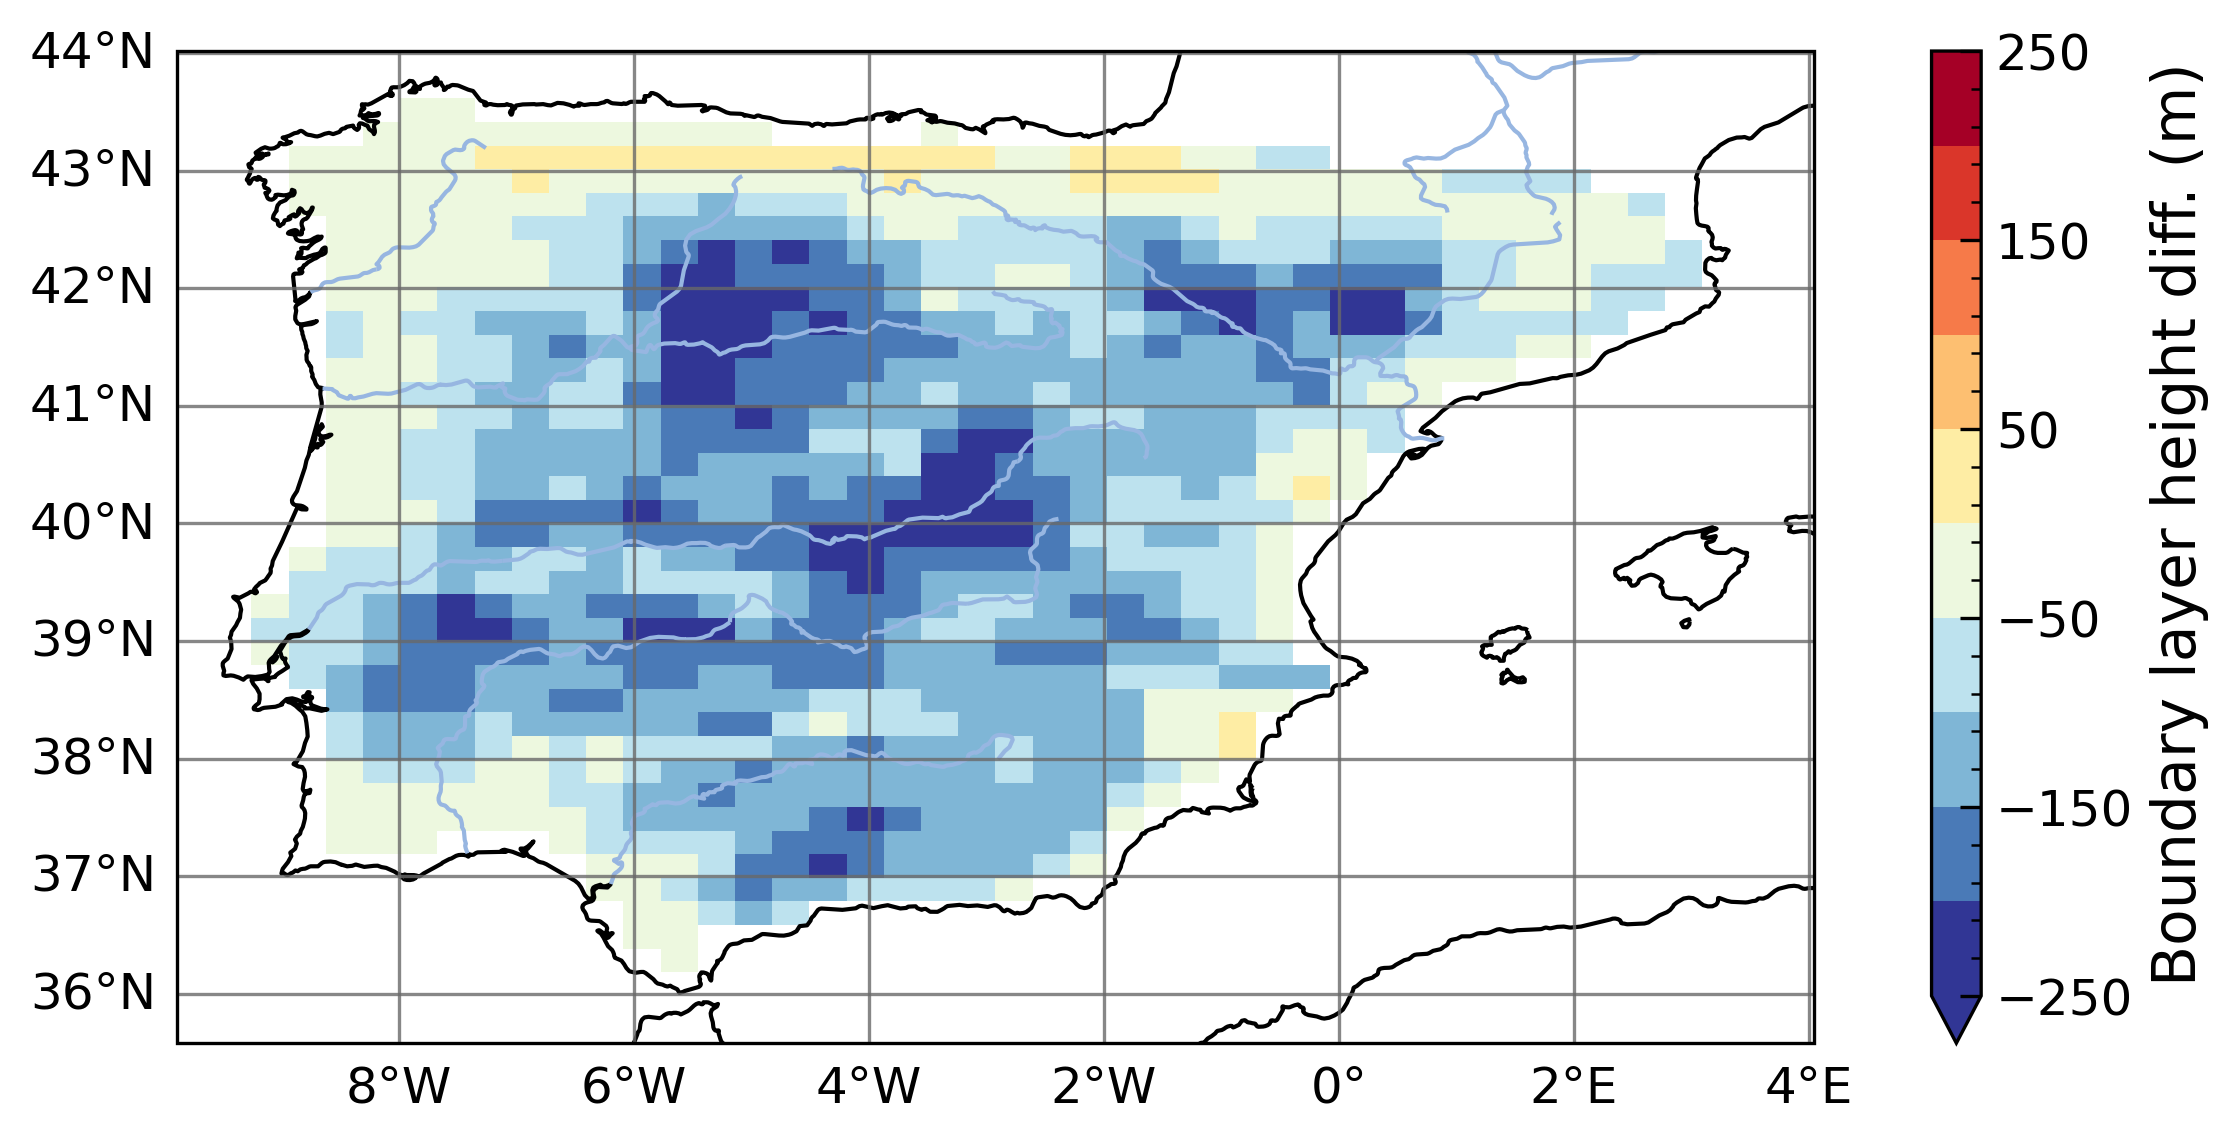
\includegraphics[width=\textwidth]{images/chap4/future/diffmap_JJA_s_pblh_futirr.png}
        \end{subfigure} &
        %lcl
        \begin{subfigure}[b]{0.5\textwidth}
            \caption{}
            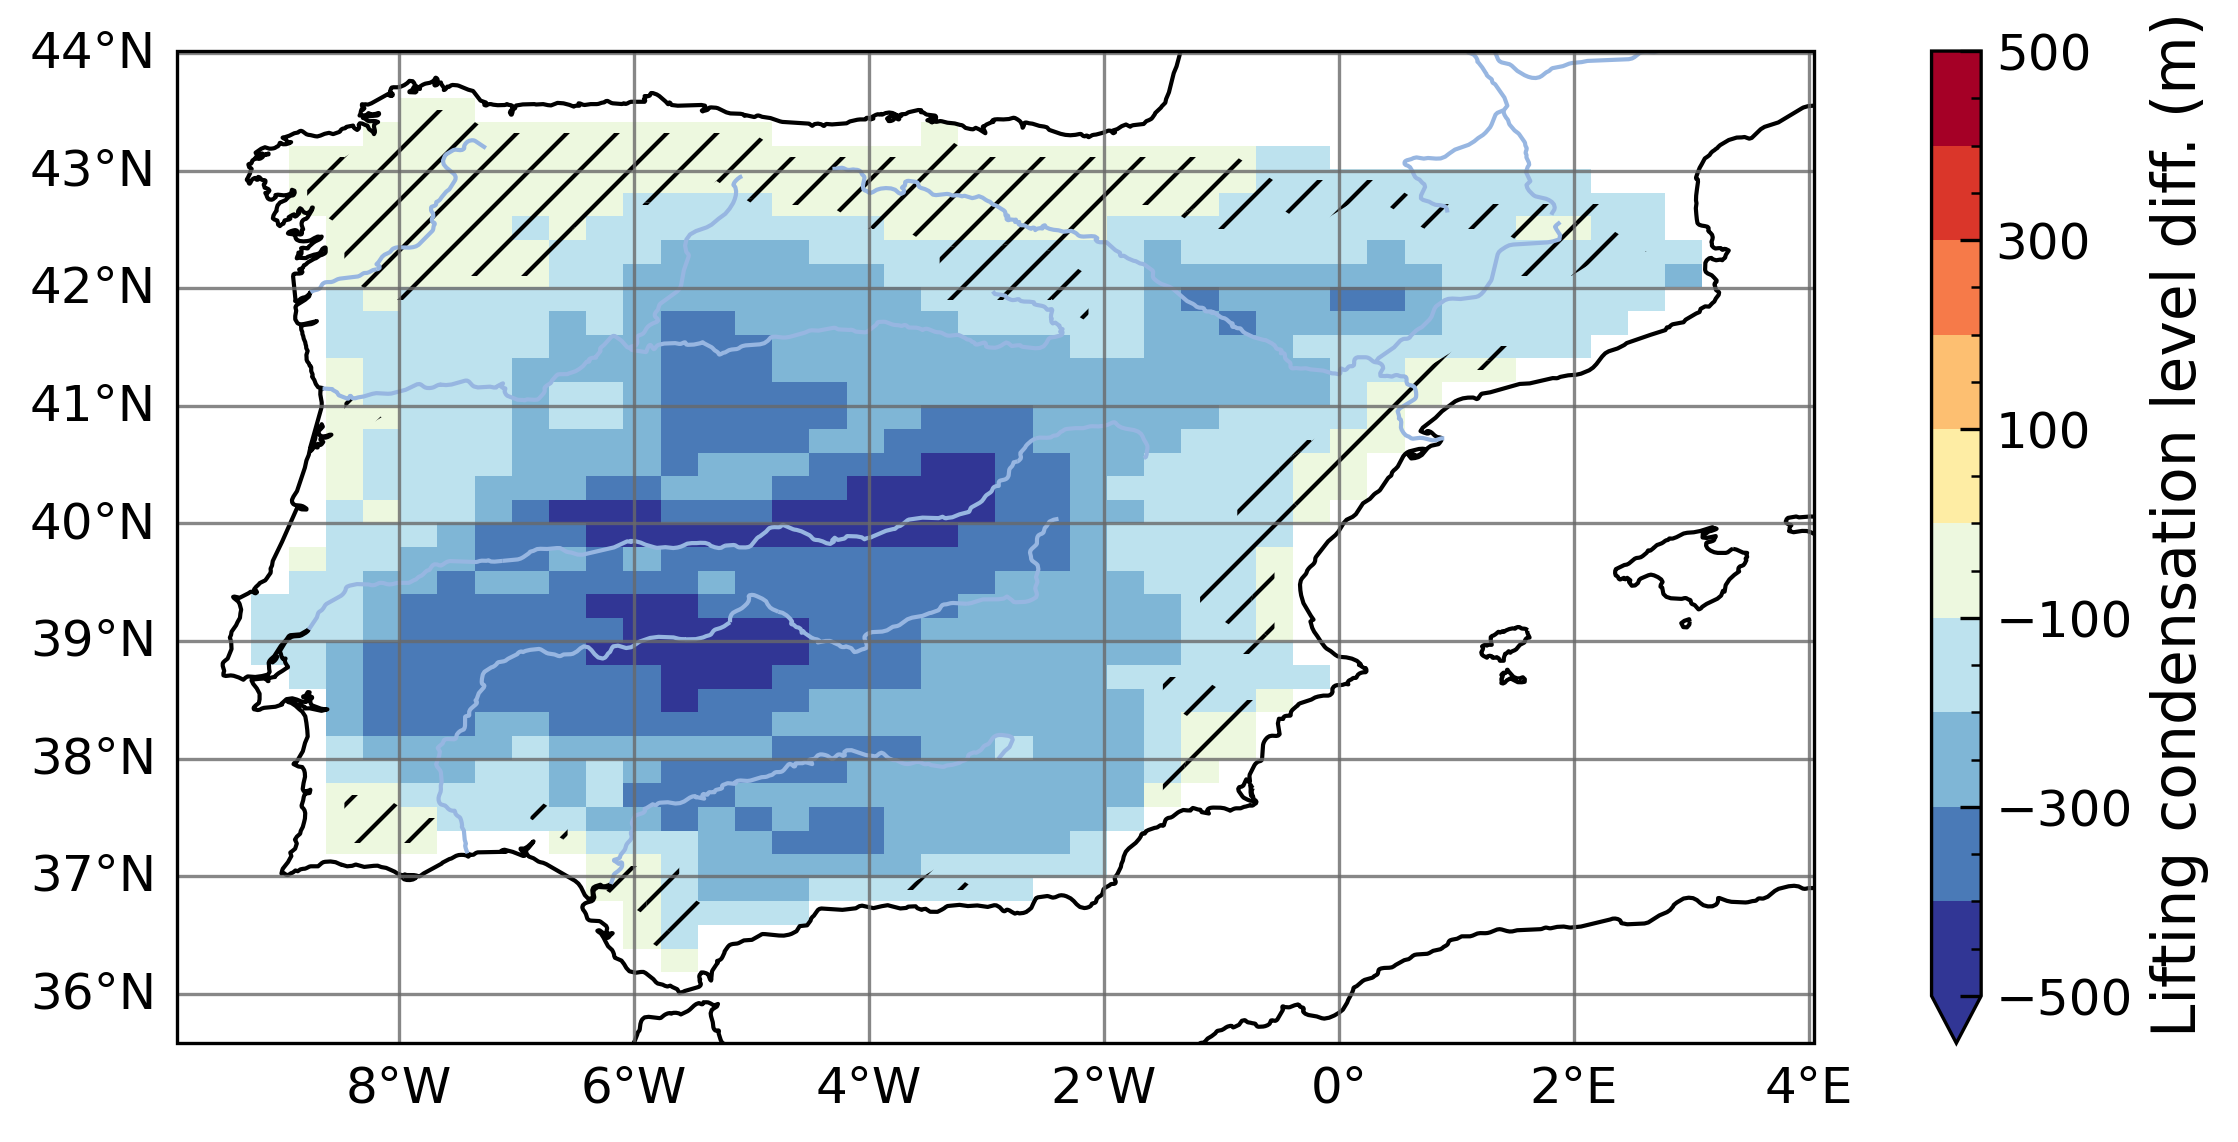
\includegraphics[width=\textwidth]{images/chap4/future/diffmap_JJA_s_lcl_futirr.png}
        \end{subfigure} \\
    \end{tabular}
    \caption{JJA}
    \label{fig:diffmaps_JJA_future_irr}
\end{figure}